\documentclass[]{phdthesis}
\addbibresource{thesis_n.bib}

\degree{Doctor of Philosophy}
\university{University College London}
\title{Computational design and\\[0.2em]characterisation of synthetic\\[0.2em] genetic switches}
\author{Miriam Leon}
\primarysupervisor{Dr. Chris P Barnes}
\secondarysupervisor{Prof. Geraint MH Thomas}

%%  Abbreviations entries  -----------------%%
%\acrlong{ } whole phrase, \acrshort{ } acronym, \acrfull{ } both
\makeglossaries
\newacronym{ode}{ODE}{Ordinary differential equation}
\newacronym{abc}{ABC}{Approximate Bayesian Computation}
\newacronym{smc}{SMC}{Sequential Monte Carlo}
\newacronym{mcmc}{MCMC}{Markov Chain Monte Carlo}
\newacronym{sde}{SDE}{Stochastic differential equation}
\newacronym{mjp}{MJP}{Markov jump process}
\newacronym{gpu}{GPU}{Graphical Processing Unit}

\newacronym{pdf}{PDF}{probability density function}


\newacronym{qssa}{QSSA}{quasi-steady state approximation}


\newacronym{cs-ma}{CS-MA}{Mass action classic switch}
\newacronym{dp-ma}{DP-MA}{Mass action double positive switch}
\newacronym{sp-ma}{SP-MA}{Mass action single positive switch}
\newacronym{cs-lu}{CS-LU}{Lu classic switch}
\newacronym{sp-lu}{SP-LU}{Lu single positive switch}
\newacronym{dp-lu}{DP-LU}{Lu double positive switch}
\newacronym{kde}{KDE}{Kernel density estimation}
%\newacronym{1d}{1D}{one dimensional}
%\newacronym{2d}{2D}{two dimensional}

\newacronym{atc}{ATc}{anhydrotetracycline}
\newacronym{iptg}{IPTG}{Isopropyl-beta-D-thiogalactopyranoside}




%%---------------------------------------------------%%
\begin{document}
% front matter
\maketitle


\begin{abstract}
\end{abstract}

\tableofcontents*
\listoffigures
\listoftables
\glossarystyle{list}

\printglossary[type=\acronymtype, title=Abbreviations, toctitle=Abbreviations]

%\printglossary[type=\acronymtype, title=Abbreviations, toctitle=Abbreviations]

\begin{acknowledgements}
\end{acknowledgements}

%% --------------------------------------------------------------
%% CHAPTERS
%% --------------------------------------------------------------

%% Introduction -------------------------------------%%
\mainmatter*
\chapter{Introduction}
\section{Contents of this thesis}


%% Background -------------------------------------%%
\mainmatter*
\chapter{Background}

\section{Introduction to synthetic biology}

Synthetic biology aims at the rational design and construction of biological parts, devices, and systems in order to engineer organisms to perform new tasks~\autocite{Lu:2009ez,Andrianantoandro:2006bi}. A part is a basic unit, like a promoter or a ribosome binding site that when combined with other parts will make a functional unit, a device~\autocite{Heinemann:2006ht}. A device processes inputs, performs functions and produces outputs~\autocite{Andrianantoandro:2006bi}. A system comprises of a collection of devices.     

Emphasis is put on the use of engineering principles such as modularity, standardisation, use of predictive models and the separation of design and construction~\autocite{Agapakis:2009bt, Heinemann:2006ht}. A hierarchy similar to computer science is used, with cells, pathways and biochemical reactions acting as computers, modules and gates respectively~\autocite{Andrianantoandro:2006bi}. 
       
Numerous applications of synthetic biology have emerged, from altering existing metabolisms to producing synthetic drugs ~\autocite{Holtz:2010bm} or creating new synthetic life forms ~\autocite{Agapakis:2009bt}. Despite the successes there is still a lack of predictive power due to the stochasticity and lack of complete knowledge of the cellular environment ~\autocite{Andrianantoandro:2006bi}.

Synthetic biology is now entering an age where simple synthetic circuits have been built, such as toggle switches \autocite{Gardner:2000vha, Kramer:2004kq, Isaacs:2003ht, Ham:2008hh, Deans:2007cya, Friedland:2009ce}, oscillators~\autocite{Stricker:2008jqa, Fung:2005jd, Tigges:2009jx} and pulse generators~\autocite{Basu:2004gn}, but larger circuits have proven more difficult \autocite{XXX}. The leap from building low-level circuits to assembling them into complex networks has yet to be made successfully~\autocite{Lu:2009ez}, and predictable circuit behaviour remains challenging \autocite{XXX}. Efforts to do so are plagued by intra-circuit crosstalk and incompatibility, as well as cellular noise, which can render synthetic networks non-functional \textit{in vivo} \autocite{XXX}. 

\section{System design in synthetic biology}

Creating synthetic devices that are robust to changing cellular contexts will be key to the success of synthetic biology. Unknown initial conditions and parameter values as well as the variability of the cellular environment, extracellular noise and crosstalk makes the majority of synthetic genetic devices non-functional~\autocite{Chen:2009ea}. Designing devices robust to this environment will lead to reliable behaviour of the systems.
When faced with a set of competing designs for a given genetic circuit, one is likely to choose the simplest possible model that can achieve the desired behaviour. However, simple systems are often the least robust. Feedback loops are well known key regulatory motifs ~\autocite{Brandman:2005ci}. Negative feedback loops are essential for homeostasis and buffering ~\autocite{Thomas:1995id} thus increasing robustness to extrinsic noise sources and positive feedback loops can generate multistationarity in a system ~\autocite{Thomas:1995id}. Incorporating this kind of additional feedback interactions can make a design more robust and reliable. 
Maximising production is an important goal for a metabolic engineering project if it is to produce an economically viable substance ~\autocite{Holtz:2010bm}. Network topologies and parameter values of different toggle switch designs are explored here in order to identify the design that maximises robustness and distance between steady states. This ensures the reliable production of the product with the greatest distance between the on and off states of the switch. 
 In the future, by selecting the system components accordingly, the parameter values can be adjusted \textit{in vivo}. For example, the parameter value corresponding to the translation initiation rate can be chosen by selecting the appropriate RBS sequence which given a nucleotide sequence will produce the desired rate ~\autocite{Holtz:2010bm}, a method developed by~\textcite{Salis:2009gk}~\autocite{Salis:2009gk}. Another method to tweak the parameter values \textit{in vivo} is to select the promoter to have the strength corresponding to the levels of gene expression and repression desired. Activity of each promoter can be measured and standardised~\autocite{Kelly:2009bj} making this process possible. For a system requiring more than one promoter, these can be efficiently selected from a promoter library using a genetic algorithm created by~\textcite{Wu:2011bq} ~\autocite{Wu:2011bq}. These standardised interchangeable components with known sequence and activity are what synthetic biology classes as BioBricks ~\autocite{Kelly:2009bj,Canton:2008fv}. These can be selected and used to construct a desired system and replicate the parameter values found in the scan presented here.

The first computational approach for the tuning of robust synthetic networks was that of~\textcite{Batt:2007jl}~\autocite{Batt:2007jl} where they examined the problem of finding a subset of the parameter set for which a given property was satisfied for all the parameters. ~\textcite{Chen:2009ea}~\autocite{Chen:2009ea} used the fuzzy  dynamic game method to solve the minimax regulation design problem of synthetic genetic networks. In that method the worst case effect of all disturbances is minimised for a given network. An evolutionary algorithm has also been used to solve the robust design problem by evolving the parameters of the system in order to make it more robust to cellular disturbances by~\textcite{Chen:2011hj}~\autocite{Chen:2011hj}. The added value of the methodology presented here is that the network structure in addition to the network parameters are adjusted to select a network that can robustly create the desired behaviour.	

\section{Introduction to Biochemical Modelling}
\subsection{Graphical representation of biochemical systems}

It is common to represent coupled biochemical reactions graphically. In a graph, as shown in Figure ~\ref{fig:Toggle switch example}, nodes represent the species and the edges represent an interaction between the species it connects, in which a transcription factor directly affects the transcription of a gene ~\cite{alon:2007b}. An arrow at the end of an arc represents activation, i.e. that when the transcription factor binds to the promoter the rate of transcription of the gene increases. A flat line perpendicular to the arc at the end of an arc represents repression, i.e. that when the transcription factor binds to the promoter the rate of transcription of the gene decreases ~\cite{alon:2007b}.

\subsection{Deterministic and Stochastic modelling}

Modelling attempts to describe the elements and dynamics of the biochemical system of interest. It is a tool used for integrating knowledge and experimental data as well as for making predictions about the behaviour of the system~\autocite{wilkinson:2006}. When modelling a biochemical system it is generally assumed that the rates of a reaction are directly proportional to the concentration of the reactants, raised to the power of their stoichiometry~\autocite{wilkinson:2006}. This is known as mass-action kinetics and is used in this work to model the various systems.  
There are two main ways of modelling a system, deterministically and stochastically. Deterministic modelling utilises ordinary differential equations (ODE) and models the concentrations of the species (proteins or other molecules) by time-dependent variables~\autocite{deJong:2002ft}. Rate equations are used to model gene regulation where the rate of production of a species is a function of the concentrations of the other species~\autocite{deJong:2002ft}. When modelling deterministically the model is viewed as a system which, with sufficient knowledge of the system, its behaviour is entirely predictable. Nevertheless we are still a long way away from having complete knowledge of a system of interesting size ~\cite{wilkinson:2006}. Deterministic modelling also assumes a homogenous mixture where species concentrations vary continuously and deterministically, assumptions that often are not met \textit{in vivo}. A cell is spatially and temporally separated, due to small molecule numbers and fluctuations in the timing of processes~\autocite{deJong:2002ft}.  
   
In stochastic modelling, species are measured in discrete amounts rather than concentrations and a joint probability distribution is used to express the probability that at time \textit{t} the cell contains a number of molecules of each species~\autocite{deJong:2002ft}. It takes uncertainty into account and does not assume a homogenous mix. It is thus often more appropriate for modelling cellular systems, although more computationally intensive. In stochastic systems the Gillespie algorithm is widely used to simulate the time-evolution of the state of the system~\autocite{wilkinson:2006}. The algorithm, developed by~\textcite{Gillespie:1977ww}~\autocite{Gillespie:1977ww} can be summarised in four steps:
\begin{enumerate}
\item Number of molecules in the system initialised
\item Two random numbers generated, one to determine which reaction will occur next and one to determine the time step
\item Time step increased and molecule counts updated according to Step 2 
\item Repeat from Step 2 until total simulation time reached
\end{enumerate}
   
 
\subsection{Steady state and stability}

In a steady state, the state of a system remains fixed. In non-linear systems, like the ones systems biology deals with, there is generally not an analytical solution thus the system has to be solved numerically. A stable steady state is defined as a fixed point whose nearby points approach the fixed point~\autocite{kaplan:1959}. This means that after a small perturbation the system will quickly return to the steady state. An unstable steady state is one which if the system is perturbed slightly then it moves away from the steady state~\autocite{konopka:2007}.    
 
 
\section{The genetic toggle switch}

One of the most common devices used in synthetic biology is the genetic toggle switch. A toggle switch consists of a set of transcription factors that mutually repress each other~\autocite{Gardner:2000vha}. Genetic switches play a major role in binary cell fate decisions like stem cell differentiation, as they are capable of exhibiting bistable behaviour. Bistability of a system is defined by the existence of two distinct phenotypic states but no intermediate state. Bistability is a property that is important in nature and a valuable resource to tap into in synthetic biology. It allows cells to alter their response to environmental cues and increases the overall population fitness by 'hedge-betting' the response of the population \autocite{XXX}. 

\subsection{Importance in natural systems}
In developmental processes, bistability ensures that the differentiating cell will follow one pathway, or the other, with no possible intermediate phenotypes. This is vital for the correct development of a cell in a specific pathway. One example is the trophectoderm differentiation pathway, in which a mutually inhibitory toggle switch exists between Oct3/4 and Cdx2. This determines whether an Embryonic Stem cell will differentiate into a Trophectoderm cell, if Cdx2 dominates the system, or an Inner Cell Mass cell if Oct3/4 dominates~\autocite{Niwa:2005fz}. Bistability is critical in this system as a cell must differentiate into either a trophectoderm cell or an inner cell mass cell, thus the signal to do so must be straightforward. In the case of the GATA1 and PU.1 toggle switch, the transcription factor pair controls the fate of the common myeloid progenitors, and the two possible differentiation paths are erythroid and myeloid blood cells~\autocite{Chickarmane:2009by}. The double-negative feedback loop created by the mutually repressive pair of transcription factors sustains the system in balance until an external stimulus causes one of the two transcription factors to increase in concentration. The increased concentration of one transcription factor causes the increased repression of the production of the antagonistic transcription factor, tipping the balance towards the dominance of the first transcription factor. The double negative feedback loop reinforces this dynamic and the system remains in the same state, until an external stimulus disturbs it~\autocite{FerrellJr:2002fh}.

\subsection{Uses in synthetic biology}
Despite their simplicity, toggle switches can be powerful building blocks with which to create complex responses in a synthetic network. They can be used in isolation or in tandem to create complex networks and signalling cascades. The toggle switch has been used for the regulation of mammalian gene expression~\autocite{Deans:2007cya, Kramer:2004kq}. Other synthetic applications of the toggle switch include the construction of a synthetic genetic clock~\autocite{Atkinson:2003tu}, of a predictable genetic timer~\autocite{Ellis:2009hka}, and the formation of biofilms in response to engineered stimuli~\autocite{Kobayashi:2004cv}. These applications are modifications of the classical toggle switch~\autocite{Gardner:2000vha}, and to our knowledge no application made of a cascade or collection of the switch has been successful. This would make more complex applications possible and could be used to solve real-life problems. For example, an analog-to-digital converter to translate external stimuli like the concentration of an inducer into an internal digital response, or programmable bacteria to move from point to point up different chemical gradients~\autocite{Lu:2009ez}. For a review on current circuits see~\autocite{Khalil:2010hm} and for possible future applications see~\autocite{Lu:2009ez}. This leap will be difficult to achieve before first being able to build robust and well characterised individual switches.

\subsection{Modelling the genetic toggle switch} 
The toggle switch motif has been studied extensively and there are numerous studies based on a number of different methods of modelling and analysis of the dynamics, including both deterministic and stochastic approaches. Deterministic modelling utilises ordinary differential equations (ODE) and models the concentrations of the species (proteins or other molecules) by time-dependent variables~\autocite{deJong:2002ft}. When modelling deterministically the model is viewed as a system whose behaviour is entirely predictable, given sufficient knowledge. In stochastic modelling, species are measured in discrete amounts rather than concentrations and a joint probability distribution is used to express the probability that at time \textit{t} the cell contains a number of molecules of each species~\autocite{deJong:2002ft,Wilkinson:2006td}. It takes uncertainty into account and is thus often more appropriate for modelling cellular systems, although more computationally expensive. In stochastic systems the Gillespie algorithm is widely used to simulate the time-evolution of the state of the system~\autocite{Warren:2005kea}.
\par
The conclusions drawn about the stability and robustness of the toggle switch also vary between the different modelling approaches. Numerous studies have concluded that cooperativity is a necessary condition for bistability to arise~\autocite{Gardner:2000vha, Walczak:2005ds, Warren:2004baa, Warren:2005kea, Cherry:2000wi}. However, ~\textcite{Lipshtat:2006wb} found that stochastic effects can give rise to bistability even without cooperativity in three kinds of switch; the exclusive switch, in which there can only be one repressor bound at any one time, a switch in which there is degradation of bound repressors, and the switch in which free repressor proteins can form a complex, which renders them inactive as transcription factors~\autocite{Lipshtat:2006wb}. In another study, \textcite{Ma:2012dt} found that the stochastic fluctuations in a system involving such a small number of molecules, like the toggle switch, uncovers effects that can not be predicted by the fully deterministic case~\autocite{Ma:2012dt}. In their system, the toggle switch was found to be tristable, as small number effects render the third unstable steady state stable. \textcite{Biancalani:2015vya} identified multiplicative noise as the source of bistability in the stochastic case~\autocite{Biancalani:2015vya}. ~\textcite{Warren:2005kea} concluded that the exclusive switch is always more robust than the general switch, since the free energy barrier is higher~\autocite{Warren:2005kea}. A summary of the toggle switch models is shown in Table~\ref{tab:refs}. As is clear from above, there is yet to exist a consensus on the stability a switch is capable of, and the most appropriate method of modelling it. Different methods arrive at different conclusions, creating confusion on which behaviour to be expected by the experimentalist for even a simple system like the toggle switch, consisting of just two genes. The toggle switch cannot be used as a building block of larger, more complex systems until its behaviour can be predicted accurately. Until then, designing systems with predictable behaviour will be near impossible.


\begin{table}[]
\centering
\caption{Summary of stability for the toggle switch found via different modelling approaches}
\label{tab:refs}
\rotatebox{90}{
\begin{tabular}{@{}ccccccc@{}}
\toprule
                                        & \multicolumn{3}{c}{\textbf{Simple}}                                                                                                                                            & \multicolumn{3}{c}{\textbf{Double positive autoregulation}} \\ \midrule
                                        & \textit{Stability}                             & \textit{Reference} & \textit{Notes}                                                                                           & \textit{Stability}  & \textit{Reference}  & \textit{Notes}  \\  \midrule
\multirow{3}{*}{\textbf{Deterministic}} & Monostable                                     & \autocite{Loinger:2007vma}       & \begin{tabular}[c]{@{}c@{}}no cooperativity,\\ exclusive \& general\end{tabular}                         & Bistable            & \autocite{Guantes:2008gs}        &                 \\
                                        & \multirow{2}{*}{Bistable}                      & \autocite{Gardner:2000vha}       & copperativity \textgreater 2,                                                                            & Tristable           & \autocite{Guantes:2008gs}        &                 \\
                                        &                                                & \autocite{Loinger:2007vma}       & bound repressor degradation                                                                              & 4 steady steates    & \autocite{Guantes:2008gs}        &                 \\ \midrule
\multirow{7}{*}{\textbf{Stochastic}}    & Monostable                                     & \autocite{Loinger:2007vma}       & \begin{tabular}[c]{@{}c@{}}no cooperativity, \\ weak repression\end{tabular}                             & Tristable           & \autocite{Lu:2014kc}             &                 \\
                                        & \multirow{4}{*}{Bistable}                      & \autocite{Lu:2014kc}            &                                                                                                          &                     &                     &                 \\
                                        &                                                & \autocite{Biancalani:2015vya}    & \begin{tabular}[c]{@{}c@{}}exclusive,\\ controlled by noise strength\end{tabular}                        &                     &                     &                 \\
                                        &                                                & \autocite{Lipshtat:2006wb}      & no cooperativity                                                                                         &                     &                     &                 \\
                                        &                                                & \autocite{Loinger:2007vma}       & \begin{tabular}[c]{@{}c@{}}no cooperativity,\\ exclusive \& \\ bound repression degradation\end{tabular} &                     &                     &                 \\
                                        & \multicolumn{1}{l}{\multirow{2}{*}{Tristable}} & \autocite{Loinger:2007vma}       & \begin{tabular}[c]{@{}c@{}}no cooperativity,\\ strong repression\end{tabular}                            &                     &                     &                 \\
                                        & \multicolumn{1}{l}{}                           & \autocite{Ma:2012dt}           &                                                                                                          &                     &                     &                 \\ \bottomrule 
\end{tabular}
}
\end{table} 
\clearpage



\section{Introduction to Bayesian statistics}

\begin{align*}
p(\theta|x) &= \frac{p(x|\theta)p(\theta)} {\displaystyle \int p(x|\theta)p(\theta)d\theta\frac{p(x|\theta)p(\theta)}{p(x)}}
\end{align*}

because
\begin{align*}
p(x)p(\theta|x) &= p(\theta)p(x|\theta)
\end{align*}

where $p(x|\theta)$ is the likelihood, $p(\theta)$ is the prior, and $\displaystyle \int p(x|\theta)p(\theta)d\theta$ is the evidence. This is the normalisation. 

Bayes factor: 
\begin{align*}
B_{12} = \frac{\displaystyle \int p(x|\theta, M_1)p(\theta, M_1)d\theta}{\displaystyle \int p(x|\theta, M_2)p(\theta, M_2)d\theta}
\end{align*}


In our case, O is the objective, and D is the design. Therefore:

\begin{align*}
p(O|D_1) = \int p(O|\theta,D_1)p(\theta|D_1)d\theta,
\end{align*}



This is the robustness, or evidence or marginal likelihood

\begin{align*}
p(O|D_1) &= \displaystyle \int p(O|\theta,D_1)p(\theta|D_1)d\theta, \\
p(O|D_1) &= \displaystyle \iiint_{\underline{\Theta}} p(O|\underline{\Theta})p(\underline{\Theta}|D_1)d\underline{\Theta}
\end{align*}

where $\underline{\Theta} = \{ \theta_1, \theta_2,\theta_3 \}$ 

Assuming the prior is uniform, and $a=0$:

\begin{align*}
p(O|D_1) &= \displaystyle \iiint_{\underline{\Theta}} p(O|\underline{\Theta})\frac{1}{b_1}\frac{1}{b_2}\frac{1}{b_3}d\underline{\Theta} \\
p(O|D_1) &= \frac{1}{b_1}\frac{1}{b_2}\frac{1}{b_3} \displaystyle \iiint_{\underline{\Theta}}p(O|\underline{\Theta})d\underline{\Theta}
\end{align*}


Assuming uniform likelihood:
\begin{align*}
p(O|D_1) &= \frac{1}{b_1}\frac{1}{b_2}\frac{1}{b_3} \displaystyle \iiint_{\underline{\Theta}_F}1d\theta_1\theta_2\theta_3+\frac{1}{b_1}\frac{1}{b_2}\frac{1}{b_3} \displaystyle \iiint_{\underline{\Theta}_F}Od\underline{\Theta}
\end{align*}


\subsection{Bayes' theorem}
\subsection{Bayesian inference}
\subsection{Model checking}
\subsection{Model comparison}
\subsection{Prior selection}







%% ABC-SysBio ---------------------------------------%%
\mainmatter*
\chapter{Effect or feedback loops on switch robustness }
\section{Introduction to ABC-SysBio}
\section{Methods}
\subsection{\acrshort{abc} for parameter estimation}
\subsection{\acrshort{abc} for model selection}
\section{Models of the genetic toggle switch}
\section{Results}
\subsection{Genetic toggle switch model selection}
\section{Conclusions}



%% StabilityFinder ----------------------------------%%
\mainmatter*
 
\chapter{Dynamics of multi-stable switches}
\section{Background}

Synthetic biology is now entering an age where simple synthetic circuits have been built, such as toggle switches \autocite{Gardner:2000vha, Kramer:2004kq, Isaacs:2003ht, Ham:2008hh, Deans:2007cya, Friedland:2009ce}, oscillators~\autocite{Stricker:2008jqa, Fung:2005jd, Tigges:2009jx} and pulse generators~\autocite{Basu:2004gn}, but larger circuits have proven more difficult \autocite{XXX}. The leap from building low-level circuits to assembling them into complex networks has yet to be made successfully~\autocite{Lu:2009ez}, and predictable circuit behaviour remains challenging \autocite{XXX}. Efforts to do so are plagued by intra-circuit crosstalk and incompatibility, as well as cellular noise, which can render synthetic networks non-functional \textit{in vivo} \autocite{XXX}. 
\par
A circuit must be robust to a fluctuating cellular environment and its response and sensitivity must be able to be fine tuned in order to orchestrate a network of circuits that function together. A robust circuit can tolerate the compound stochasticity that a chain of circuits brings, and fine tuning of its response and sensitivity enables the researcher to make it sensitive to an upstream signal as well as influence a downstream subsystem. Parts can be fine tuned by developing component libraries~\autocite{Lu:2009ez,}, but this will be of little use if the required parameter ranges for parts to make a functional complex network are unknown, and will only perpetuate the cycles of trial-and-error. A computational method to find the range of parameter values that will produce the behaviour of choice is crucial to the design process by enabling the informed selection of appropriate parts from the libraries. If it is known that gene expression must be low for a given stability, one can select a weak promoter or a low copy plasmid for the desired construct. 
\par
One of the most common devices used in synthetic biology is the genetic toggle switch. A toggle switch consists of a set of transcription factors that mutually repress each other~\autocite{Gardner:2000vha}. Genetic switches play a major role in binary cell fate decisions like stem cell differentiation, as they are capable of exhibiting bistable behaviour. Bistability of a system is defined by the existence of two distinct phenotypic states but no intermediate state. Bistability is a property that is important in nature and a valuable resource to tap into in synthetic biology. It allows cells to alter their response to environmental cues and increases the overall population fitness by 'hedge-betting' the response of the population \autocite{XXX}. 
\par
%In developmental processes, bistability ensures that the differentiating cell will follow one pathway, or the other, with no possible intermediate phenotypes. This is vital for the correct development of a cell in a specific pathway. One example is the trophectoderm differentiation pathway, in which a mutually inhibitory toggle switch exists between Oct3/4 and Cdx2. This determines whether an Embryonic Stem cell will differentiate into a Trophectoderm cell, if Cdx2 dominates the system, or an Inner Cell Mass cell if Oct3/4 dominates~\autocite{Niwa:2005fz}. Bistability is critical in this system as a cell must differentiate into either a trophectoderm cell or an inner cell mass cell, thus the signal to do so must be straightforward. In the case of the GATA1 and PU.1 toggle switch, the transcription factor pair controls the fate of the common myeloid progenitors, and the two possible differentiation paths are erythroid and myeloid blood cells~\autocite{Chickarmane:2009by}. The double-negative feedback loop created by the mutually repressive pair of transcription factors sustains the system in balance until an external stimulus causes one of the two transcription factors to increase in concentration. The increased concentration of one transcription factor causes the increased repression of the production of the antagonistic transcription factor, tipping the balance towards the dominance of the first transcription factor. The double negative feedback loop reinforces this dynamic and the system remains in the same state, until an external stimulus disturbs it~\autocite{FerrellJr:2002fh}.
\par
Despite their simplicity, toggle switches can be powerful building blocks with which to create complex responses in a synthetic network. They can be used in isolation or in tandem to create complex networks and signalling cascades. The toggle switch has been used for the regulation of mammalian gene expression~\autocite{Deans:2007cya, Kramer:2004kq}. Other synthetic applications of the toggle switch include the construction of a synthetic genetic clock~\autocite{Atkinson:2003tu}, of a predictable genetic timer~\autocite{Ellis:2009hka}, and the formation of biofilms in response to engineered stimuli~\autocite{Kobayashi:2004cv}. These applications are modifications of the classical toggle switch~\autocite{Gardner:2000vha}, and to our knowledge no application made of a cascade or collection of the switch has been successful. This would make more complex applications possible and could be used to solve real-life problems. For example, an analog-to-digital converter to translate external stimuli like the concentration of an inducer into an internal digital response, or programmable bacteria to move from point to point up different chemical gradients~\autocite{Lu:2009ez}. For a review on current circuits see~\autocite{Khalil:2010hm} and for possible future applications see~\autocite{Lu:2009ez}. This leap will be difficult to achieve before first being able to build robust and well characterised individual switches.
\par
The toggle switch motif has been studied extensively and there are numerous studies based on a number of different methods of modelling and analysis of the dynamics, including both deterministic and stochastic approaches. Deterministic modelling utilises ordinary differential equations (ODE) and models the concentrations of the species (proteins or other molecules) by time-dependent variables~\autocite{deJong:2002ft}. When modelling deterministically the model is viewed as a system whose behaviour is entirely predictable, given sufficient knowledge. In stochastic modelling, species are measured in discrete amounts rather than concentrations and a joint probability distribution is used to express the probability that at time \textit{t} the cell contains a number of molecules of each species~\autocite{deJong:2002ft,Wilkinson:2006td}. It takes uncertainty into account and is thus often more appropriate for modelling cellular systems, although more computationally expensive. In stochastic systems the Gillespie algorithm is widely used to simulate the time-evolution of the state of the system~\autocite{Warren:2005kea}.
\par
Both analytical and computational approaches have been deployed for the study of the toggle switch. Analytical approaches are limited to simpler models and thus require a number of assumptions to be made. The system under consideration has to be reduced to very few equations and parameters in order to make the system solvable. This requires assumptions to be made about the system that cannot always be justified, such as the quasi-steady state approximation (QSSA). The QSSA assumes that the binding/unbinding processes are much faster than any other process~\autocite{Loinger:2007vma}, thus the bound intermediate is assumed to always be in steady state. The QSSA assumption is met \textit{in vitro} but often does not hold \textit{in vivo} and its misuse can lead to large errors and incorrectly estimated parameters~\autocite{Pedersen:2007ke}. Moreover, it is generally not possible to solve even simple stochastic models analytically, and these methods are restricted to deterministic models. The computational and graph-theoretic approaches developed for the study of multistationarity generally focus on deciding on whether a given system is incapable of producing multiple steady states ~\autocite{Conradi:2007jo, Banaji:2010fh,Feliu:2013dz}. For example, ~\textcite{Feliu:2013dz} developed an approach using chemical reaction theory and generalised mass action modelling \autocite{Feliu:2013dz}. No approach exists that can handle both deterministic and stochastic systems in an integrated manner.
\par
The conclusions drawn about the stability and robustness of the toggle switch also vary between the different modelling approaches. Numerous studies have concluded that cooperativity is a necessary condition for bistability to arise~\autocite{Gardner:2000vha, Walczak:2005ds, Warren:2004baa, Warren:2005kea, Cherry:2000wi}. However, ~\textcite{Lipshtat:2006wb} found that stochastic effects can give rise to bistability even without cooperativity in three kinds of switch; the exclusive switch, in which there can only be one repressor bound at any one time, a switch in which there is degradation of bound repressors, and the switch in which free repressor proteins can form a complex, which renders them inactive as transcription factors~\autocite{Lipshtat:2006wb}. In another study, \textcite{Ma:2012dt} found that the stochastic fluctuations in a system involving such a small number of molecules, like the toggle switch, uncovers effects that can not be predicted by the fully deterministic case~\autocite{Ma:2012dt}. In their system, the toggle switch was found to be tristable, as small number effects render the third unstable steady state stable. \textcite{Biancalani:2015vya} identified multiplicative noise as the source of bistability in the stochastic case~\autocite{Biancalani:2015vya}. ~\textcite{Warren:2005kea} concluded that the exclusive switch is always more robust than the general switch, since the free energy barrier is higher~\autocite{Warren:2005kea}. A summary of the toggle switch models is shown in Table~\ref{tab:refs}. As is clear from above, there is yet to exist a consensus on the stability a switch is capable of, and the most appropriate method of modelling it. Different methods arrive at different conclusions, creating confusion on which behaviour to be expected by the experimentalist for even a simple system like the toggle switch, consisting of just two genes. The toggle switch cannot be used as a building block of larger, more complex systems until its behaviour can be predicted accurately. Until then, designing systems with predictable behaviour will be near impossible.
\par
Here we present a computational framework based on sequential Monte Carlo that takes a model and determines whether it is capable of producing a given number of (stable) steady states and the parameter space that gives rise to the behaviour. Uniquely, this can be done for both deterministic and stochastic models, and also complex models with many parameters, thus removing the need for simplifying assumptions. Our framework can be used for comparing the conclusions drawn by various modelling approaches and thus provides a way to investigate appropriate abstractions. We have made this framework into a python package, called StabilityFinder. This methodology is used to investigate genetic toggle switches and uncover the design principles behind making a bistable switch, as well as those necessary to make a tristable switch. We find that degradation rates of transcription factors are important for bistability, and that the addition of positive autoregulation can create tristable behaviour and also significantly more robust bistability when feedback strength is well balanced. Modelling transcription and translation allows us to conclude that transcriptional bursting can inhibit bistability, and also that bistability can occur even when the assumptions of time scale separation in the repressor dynamics are not met. We also examine the design principles behind the design of bistable versus tristable switches and highlight the importance of including stochastic dynamics when modelling these systems. Finally we demonstrate the ability of the framework to examine more complex systems and examine the design principles of a three gene switch. These examples demonstrate that StabilityFinder will be a valuable tool in the future design and construction of novel gene networks. 

\begin{table}[]
\centering
\caption{Summary of stability for the toggle switch found via different modelling approaches}
\label{tab:refs}
\rotatebox{90}{
\begin{tabular}{@{}ccccccc@{}}
\toprule
                                        & \multicolumn{3}{c}{\textbf{Simple}}                                                                                                                                            & \multicolumn{3}{c}{\textbf{Double positive autoregulation}} \\ \midrule
                                        & \textit{Stability}                             & \textit{Reference} & \textit{Notes}                                                                                           & \textit{Stability}  & \textit{Reference}  & \textit{Notes}  \\  \midrule
\multirow{3}{*}{\textbf{Deterministic}} & Monostable                                     & \autocite{Loinger:2007vma}       & \begin{tabular}[c]{@{}c@{}}no cooperativity,\\ exclusive \& general\end{tabular}                         & Bistable            & \autocite{Guantes:2008gs}        &                 \\
                                        & \multirow{2}{*}{Bistable}                      & \autocite{Gardner:2000vha}       & copperativity \textgreater 2,                                                                            & Tristable           & \autocite{Guantes:2008gs}        &                 \\
                                        &                                                & \autocite{Loinger:2007vma}       & bound repressor degradation                                                                              & 4 steady steates    & \autocite{Guantes:2008gs}        &                 \\ \midrule
\multirow{7}{*}{\textbf{Stochastic}}    & Monostable                                     & \autocite{Loinger:2007vma}       & \begin{tabular}[c]{@{}c@{}}no cooperativity, \\ weak repression\end{tabular}                             & Tristable           & \autocite{Lu:2014kc}             &                 \\
                                        & \multirow{4}{*}{Bistable}                      & \autocite{Lu:2014kc}            &                                                                                                          &                     &                     &                 \\
                                        &                                                & \autocite{Biancalani:2015vya}    & \begin{tabular}[c]{@{}c@{}}exclusive,\\ controlled by noise strength\end{tabular}                        &                     &                     &                 \\
                                        &                                                & \autocite{Lipshtat:2006wb}      & no cooperativity                                                                                         &                     &                     &                 \\
                                        &                                                & \autocite{Loinger:2007vma}       & \begin{tabular}[c]{@{}c@{}}no cooperativity,\\ exclusive \& \\ bound repression degradation\end{tabular} &                     &                     &                 \\
                                        & \multicolumn{1}{l}{\multirow{2}{*}{Tristable}} & \autocite{Loinger:2007vma}       & \begin{tabular}[c]{@{}c@{}}no cooperativity,\\ strong repression\end{tabular}                            &                     &                     &                 \\
                                        & \multicolumn{1}{l}{}                           & \autocite{Ma:2012dt}           &                                                                                                          &                     &                     &                 \\ \bottomrule 
\end{tabular}
}
\end{table} 
\section{Methods}
\subsection{StabilityFinder}

The framework is based on a statistical inference method which combines \acrfull{abc} with \acrfull{smc} \autocite{Toni:2009tr}. This simulation-based method uses an iterative process to arrive at a distribution of parameter values that can give rise to observed data or a desired system behaviour \autocite{Barnes:2011hh}.
\acrshort{abc} methods are used for inferring the posterior distribution in cases where it is too computationally expensive to evaluate the likelihood function. Instead of calculating the likelihood, \acrshort{abc} methods simulate the data and then compare the simulated and observed data through a distance function \autocite{Toni:2009tr}. Given the prior distribution $\pi(\theta)$ we can approximate the posterior distribution, $\pi(\theta\mid x)\propto f(x\mid\theta)\pi(\theta)$, where $f(x\mid\theta)$ is the likelihood of a parameter, $\theta$, given the data, $x$. There are a number of different variations of the \acrshort{abc} algorithm depending on how the the approximate posterior distribution is sampled. 
\par
The simplest \acrshort{abc} algorithm is the \acrshort{abc} rejection sampler~\autocite{Pritchard:1999td}. In this method, parameters are sampled from the prior and data simulated thorough the data generating model. For each simulated data set, a distance from that of the desired behaviour is calculated, and if greater than a threshold, $\epsilon$, the sample is rejected, otherwise it is accepted. 
\begin{algorithm}[H]
	\label{alg:ABC}
  \caption{ABC rejection algorithm}
 \begin{algorithmic}[1]
    \Statex
	\State Sample a parameter vector $\theta$ from prior $\pi(\theta)$
	\State Simulate the model given $\theta$
    \State Compare the simulated data with the desired data, using a distance function $d$ and tolerance $\epsilon$. if $d \leq \epsilon$, accept $\theta$ 
   
  \end{algorithmic}
\end{algorithm}
\noindent The main disadvantage of this method is that if the prior distribution is very different from the posterior, the acceptance rate is very low~\autocite{Toni:2009tr}. An alternative method is the \acrshort{abc} \acrfull{mcmc} developed by~\textcite{Marjoram:2003up}~\autocite{Marjoram:2003up}. The disadvantage of this method is that if it gets stuck in an area of low probability it can be very slow to converge~\autocite{Sisson:wf}. 
The method used here is based on sequential Monte Carlo, which avoids both issues faced by the rejection and MCMC methods. It propagates the prior through a series of intermediate distributions in order to arrive at an approximation of the posterior. The tolerance, $\epsilon$ for the distance of the simulated data to the desired data is made smaller at each iteration. When $\epsilon$ is sufficiently small, the result will approximate the posterior distribution~\autocite{Toni:2009tr}.  
\par
To investigate the multistable behaviour of systems, a number of extensions to existing approaches are required. For a given set of parameter values, sample points are taken across initial conditions using latin hypercube sampling \autocite{XXX}, and the ensemble system simulated in time until steady state. The distance function in \acrshort{abc} is replaced by a distance on the desired stability of the simulated model. To do this we cluster the steady state coordinates using k means clustering and use the gap statistic to determine the number of clusters \autocite{XXX}. The algorithm is summarised below.
\begin{algorithm}[H]
\label{alg:StabilityFinder}
\caption{StabilityFinder algorithm}
 \begin{algorithmic}[1]
    \Statex
	\State Initialise $\epsilon$ 
	\Let{population p}{1}
	\If{p $= 1$}
		\State Sample particles ($\theta$ ) from priors
		\Else
			\State Sample particles from previous population
			\State Perturb each particle by $\pm$ half the range of the previous population (j) to obtain new perturbed population (i).
	\EndIf
	\State Sample initial conditions via Latin Hypercube Sampling.
    \State Simulate each particle to obtain steady state values.
    \State Cluster steady state
	\State Reject particles if d $\textgreater$ $\epsilon$.
    \State Calculate weight for each accepted $\theta$
	%\State $w_{t}^{(i)} = \begin{cases} 1, & \mbox{if } p = 0 \\\frac{\pi(\theta_{t}^{(i)})}{\sum_{j=1}^N w_{t-1}^{(j)} K_{t}(\theta_{t-1}^{(j)}, \theta_{t}^{(i)})}, and \mbox{if } p \geq  0. \end{cases}$
	\State Normalise weights
	\Repeat{steps 3 - 15} \Until{$\epsilon \leq \epsilon_T$}
  \end{algorithmic} 
\end{algorithm}
\noindent This algorithm is available as a Python package, called StabilityFinder. %which is available at \url{https://github.com/ucl-cssb/StabilityFinder.git}.  
The user provides an SBML model file \autocite{XXX} and an input file that contains all the necessary information to run the algorithm, including the desired stability and the final tolerance, $\epsilon$, for the distance from the desired behaviour necessary for the algorithm to terminate. The flow of execution is illustrated in Figure~\ref{fig:fig1}. Since the algorithm is computationally intensive, all deterministic and stochastic simulations are performed using algorithms implemented on \acrfull{gpu}s \autocite{XXX}.

\subsection{Calculating robustness}
We use the results from StabilityFinder to estimate system robustness by comparing the volume of the posterior to the volume of the prior within a given model. This is done using a Monte Carlo sampling rejection algorithm by taking random samples from the prior and accepting those found in the functional region $F$ (or posterior distribution). Robustness is then defined as the number of accepted samples divided by the total number of samples.
\begin{algorithm}[ht]
	\label{alg:robustness}
  \caption{Calculating robustness via Monte Carlo sampling rejection }
 \begin{algorithmic}[1]
    \Statex
    \State Sample from priors 
    \State Get min and max boundaries of functional region of posterior ($F$)
	\If{sample within $F$}
    	\State $accepted += 1$
    \EndIf
    	    	
    \State $acceptance\_rate$ = $\frac{accep
    	ted}{number of samples}$
    \State \Return $acceptance\_rate$
    
  \end{algorithmic}
\end{algorithm}	



\section{Testing StabilityFinder}

\textcite{Gardner:2000vha} constructed the first synthetic genetic toggle switch~\autocite{Gardner:2000vha}. Their model consisted of two mutually repressing transcription factors, as shown in Figure~\ref{fig:fig2}A, and in the deterministic case is defined by the following \acrshort{ode}s.
\begin{align*}
\frac{du}{dt} &= \frac{a_1}{1+v^{\beta}} - u\\
\frac{dv}{dt} &= \frac{a_2}{1+u^{\gamma }} - v,
\end{align*}
where \textit{u} is the concentration of repressor 1, \textit{v} the concentration of repressor 2, $a_1$ and $a_2$ denote the effective rates of synthesis of repressors 1 and 2 respectively,  \textit{$\beta$} is the cooperativity of repression of promoter 1 and \textit{$\gamma$} of repressor 2. Gardner \textit{et al} studied the deterministic case and concluded that there are two conditions for bistability for this model; that $a_1$ and $a_2$ are balanced and that $\beta$, $\gamma$ \textgreater 1 \autocite{Gardner:2000vha}. In order to test StabilityFinder we used it to find the posterior distribution for which this model exhibits bistable behaviour. We therefore set the desired behaviour to two (stable) steady states, and using a wide range of values as priors as shown in the Supplementary Information, we used StabilityFinder to find the parameter values necessary for bistability to occur. The posterior distribution calculated by StabilityFinder for the Gardner deterministic case is shown in Figure~\ref{fig:fig2}B.
\par
These results agree with the results reported by~\textcite{Gardner:2000vha}~\autocite{Gardner:2000vha}. For this switch to be bistable $a_1$ and $a_2$ must be balanced while $\beta$ and $\gamma$ must both be \textgreater 1, as can be seen in the marginal distributions of $\beta$ and $\gamma$ in Figure~\ref{fig:fig2}B. The conditions set by the original paper for parameters $a_1$ and $a_2$ are met, as the joint distribution shown in Figure~\ref{fig:fig2}B matches the bifurcation lines calculated in the original paper {\color{red} How do you know, did you calculate these? I think you should try and plot them on the posterior}. 
We next applied StabilityFinder to the case of the Gardner switch under stochastic dynamics using the same priors as the deterministic case, and again searched the parameter space for bistable behaviour. The posterior is shown in Figure~\ref{fig:fig2}C. We can see that the conditions on the parameters required for bistability in the deterministic case generally still stand in the stochastic case. There appears to be slightly looser requirements on the parameters of the stochastic model (wider marginal distributions), which is expected due to the nature of clustering deterministic steady states versus stochastic steady states. The gap statistic is used in the case of the stochastic case, as it is capable of dealing with noisier data whereas a simpler and faster algorithm is used for clustering the deterministic solutions. The study on the effect of the clustering methods on robustness is shown in the Supplementary Information. These results demonstrate that StabilityFinder can be used to find the parameter values that can produce a desired stability and allow us to confidently apply the methodology to more complex models.

\begin{table}[h]
\centering
\caption{Gardner switch priors in the deterministic and stochastic cases}
\label{tab:gard_det_stoch}
\begin{tabular}{@{}cccccc@{}}
\toprule
\multicolumn{4}{c}{Parameters}                          & \multicolumn{2}{c}{Species} \\ \cmidrule(lr){1-4}
\cmidrule(lr){5-6}
$a_1$ & $\beta$ & $a_2$ & \multicolumn{1}{c}{$\gamma$} & $s_1$        & $s_2$        \\
0-60  & 0-5     & 0-60  & 0-5                           & 0-100        & 0-100        \\ \bottomrule
\end{tabular}
\end{table}

\section{Lu toggle switch models}

We next analyzed an extension of the Gardner switch model developed by~\textcite{Lu:2014kc}~\autocite{Lu:2014kc}. They considered two types of switches, the classic switch consisting of two mutually repressing transcription factors (model \acrshort{cs-lu}), as well as a \acrfull{dp-lu}.  The classical switch was found to be bistable given the set of parameters used, while the DP switch was found to be tristable ~\autocite{Lu:2014kc}. The classical model used in their study is given by the following system of \acrshort{ode}s.
\begin{align*}
\dot{x} & = g_{x}\, H^{S}_{xy}(y) -k_{x}x \\
\dot{y} & = g_{y}\,H^{S}_{yx}(x) -k_{y}y,
\end{align*}
where
\begin{align*}
H^{S}_{I}(x) &= H^{-}_{I}(x)+\lambda_{I}H^{+}_{I}(x) \\
H^{-}_{I}(x) &= 1 \big/\left[1+(x/x_{I})^{n_{I}}\right] \\
H^{+}_{I}(x) &= 1-H^{-}_{I}(x),
\end{align*}
and $g_I$ represents the production rate, $k_I$ the degradation rate, $n_I$ the Hill coefficient, $x_I$ the Hill threshold concentration and $\lambda_I$ the fold change of the transcription rates, and $I\in\{xy, yx, xx, yy\}$. 
\par
For the parameter values used in the Lu study, the classical switch exhibits three steady states (Figure~\ref{fig:fig3}), two of which are stable and one is unstable. Using StabilityFinder with priors centred around the parameter values used in the original paper (see Supplementary Information), we can identify the most important parameters for achieving bistability. The posterior distribution of these models are shown in Figure~\ref{fig:fig3}A. We find that the parameters representing the rates of degradation of the transcription factors in the system ($k_x$,$k_y$) must both be large in relation to the prior ranges for bistability to occur. Protein degradation rates have been shown to be important for many system behaviours including oscillations \autocite{XXX}. {\color{red} Anything else regarding this classical model? with more parameters}

It is known that that the addition of positive autoregulation to the classical toggle switch can induce tristability  \autocite{XXX, Lu:2014kc}. Here we investigate the interplay of positive autoregulation on the values of the other parameters in the model. We extended the analysis presented in ~\textcite{Lu:2014kc} by including the switch with single positive autoregulation (model \acrshort{sp-lu}), where an asymmetry of positive feedbacks is present between the two genes. The advantage of using StabilityFinder over solving the system analytically is that the full parameter space is explored rather than solving the system for a single set of parameters. This allows us to deduce model properties that could not otherwise be identified. Robustness to parameter fluctuations can be explored, as well as parameter correlations and restrictions on the values they can take while still producing the desired behaviour.  
\par
The \acrshort{dp-lu} model is given by
\begin{align*}
\dot{x} = f_{x}(x,y) &= g_{x}\, H^{S}_{xy}(y)\, H^{S}_{xx}\,(x)-k_{x}x \\
\dot{y} = f_{y}(x,y) &= g_{y}\,H^{S}_{yx}(x)\,H^{S}_{yy}\,(y)-k_{y}y,
\end{align*}
whereas the \acrshort{cs-lu} switch is modelled using the following \acrshort{ode} system
\begin{align*}
\dot{x} & = g_{x}\, H^{S}_{xy}(y)\, H^{S}_{xx}\,(x)-k_{x}x \\
\dot{y} & = g_{y}\,H^{S}_{yx}(x) - k_{y}y.
\end{align*}
We find that the switch with single positive autoregulation is capable of bistable behaviour as seen in Figure~\ref{fig:fig3}B, but this is only possible when the strength of the promoter under positive autoregulation, $gx$, is small. There appear to be no such constraints on the strength of the original, unmodified, promoter, $gy$.  
\par
Upon examination of the \acrshort{dp-lu} model, we also find that tristability in the switch is relatively robust, as tristability is found across a large range of parameter values, with no parameters strongly constrained {\color{red} Can we say a bit more here?}. Two types of tristable behaviour are identified, one where the third steady state is at (0,0) and and one where the third steady state has non-zero values. This result agrees with previous work by~\textcite{Guantes:2008gs}, who found that a switch can exhibit two kinds of tristability, one in which the third steady state is high (\RNum{3}$_H$) and one in which it is low (\RNum{3}$_L$)~\autocite{Guantes:2008gs}. %The difference between the two tristable switches is explored in a later section. 

deterministic dynamics~\autocite{Guantes:2008gs}. The classical switch is also capable of both bistable and tristable behaviour when stochastic dynamics capture small number effects~\autocite{Ma:2012dt}. It is therefore of great interest to understand the conditions under which these two behaviours occur in both stochastic and deterministic scenarios. 
\par
In order to do this using StabilityFinder, we first obtained posterior distributions for bistable and tristable behaviours in the deterministic case (\acrshort{dp-lu} model) and then compared the individual parameter distributions (Figure~\ref{fig:fig6} and Supplementary Information). From analysis of the one dimensional marginal distributions it appears that there is no difference in the parameter values that allow a switch to be bistable versus tristable (Figure~\ref{fig:fig6}B). However, upon examination of the two dimensional marginal distributions we find that the correlation structure of a small subset of the posterior parameter values is in fact different under the two behaviours (Figure~\ref{fig:fig6}C). Most notably, we find differences in the bivariate distribution of the two parameters for gene expression, $gx$ and $gy$, as highlighted in Figure~\ref{fig:fig6}C, box 1. In the tristable case the distribution is more constrained than in the bistable case, as both parameters must be small for tristability to arise. 
Parameters $xYY$ and $gy$ are tightly constrained in the tristable case and both required to be small, but less so in the bistable case (Figure~\ref{fig:fig6}C, box 3). Another notable difference is between parameters $xXX$ and $lXX$ shown in Figure~\ref{fig:fig6}C, box 4, where they are constrained in the bistable case but not the tristable case. Interestingly, we also find parameter correlations conserved between the bistable and tristable case, as seen in Figure~\ref{fig:fig6}C, box 2, where parameters $lXX$ and $gx$, positive autoregulation and gene expression are negatively correlated in both cases.  This highlights the importance of treating unknown parameters as distributions rather than fixed values when studying the parameter values of a model, as they are capable of uncovering not only the ranges and values needed but also the correlations between parameters that would not have otherwise been detected.

To further demonstrate the flexibility of our framework we investigated a system capable of higher stabilities. Multistability is found in differentiating pathways, like the myeloid differentiation pathway~\autocite{Ghaffarizadeh:2014bt, Cinquin:2005go}. We allow for these more complex dynamics by extending the Lu DP model by adding another gene, making it a three gene switch.  This new system is depicted in Figure~\ref{fig:fig8}A. In StabilityFinder we look for six steady states, the output being in nodes $X$ and $Y$ and using the priors shown in Table~\ref{tab:multi_priors}. We successfully find that the system is capable of six steady states, as shown in Figure~\ref{fig:fig8}C and as predicted mathematically and shown in Figure~\ref{fig:fig8}B. Interestingly, and consistent with the results presented above, we find that the most constrained parameters for this behaviour are again the degradation rate of the proteins, $kx$. Additionally we find that the Hill coefficients for the repressors, $nxy$, are tightly contrained to be smaller than 1.5 as seen in Figure~\ref{fig:fig8}D. {\color{red} What else can we do here? Can we simulate the system switching or something?} This example demonstrates that StabilityFinder can be used to elucidate the dynamics of more complex network architectures, which will be key to the successful design and construction of novel gene networks as synthetic biology advances.

\begin{table}[htpb]
\centering
\caption{Priors of the classical(\acrshort{cs-lu}), single positive (\acrshort{sp-lu}) and double positive (\acrshort{dp-lu}) models.}
\label{tab:lu_all}
\begin{tabular}{@{}ccccc@{}}
\toprule
Parameter                                            & Symbol & \acrshort{cs-lu}       & \acrshort{sp-lu}        & \acrshort{dp-lu}       \\ \midrule
\multirow{2}{*}{Production rate}                & gx        & 30-50   & 1-2       & 1-100    \\
                                                & gy        & 30-50   & 20-25     & 1-100    \\[4pt]
\multirow{2}{*}{Degradation rate}               & kx        & 0-0.5   & 50-55     & 0-1      \\
                                                & ky        & 0-0.5   & 48-52     & 0-1      \\[4pt]
\multirow{2}{*}{Hill coefficient}               & nxy       & 1-5     & 30-35     & 0-10     \\
                                                & nyx       & 1-5     & 0.1-0.2   & 0-10     \\[4pt]
\multirow{2}{*}{Hill thresholds concentration}  & xxy       & 100-300 & 2-3       & 100-1000 \\
                                                & xyx       & 100-300 & 0.4-0.6   & 100-1000 \\[4pt]
\multirow{2}{*}{Transcription rate fold change} & lxy       & 0-0.5   & 0.02-0.04 & 0-1      \\
                                                & lyx       & 0-0.5   & 0.02-0.04 & 0-0.2    \\[4pt]
\multirow{2}{*}{Hill coefficient}               & nXX       & -       & 25-30     & 0-10     \\
                                                & nYY       & -       & 0.01-0.02 & 0-10     \\[4pt]
\multirow{2}{*}{Hill thresholds concentration}  & xXX       & -       & 0.4-0.5   & 50-500   \\
                                                & xYY       & -       & 1-3       & 50-500   \\[4pt]
\multirow{2}{*}{Transcription rate fold change} & lXX       & -       & 65-72     & 1-20     \\
                                                & lYY       & -       & 0.02-0.04 & 1-20     \\ \hline
\end{tabular}
\end{table}


\begin{table}[htpb]
\centering
\caption{Priors used in the three-node switch}
\label{tab:multi_priors}
\begin{tabular}{@{}ccc@{}}
\toprule
Parameter                           & Symbol & Range   \\ \midrule
Production rate                & gx        & 3-5    \\
Degradation rate               & kx        & 0-0.2     \\
Hill coefficient               & nxy       & 0-2    \\
Hill thresholds concentration  & xxy       & 140-160 \\
Transcription rate fold change & lxy       & 0-0.2     \\
Hill coefficient               & nxx       & 2-4     \\
Hill thresholds concentration  & xxx       & 90-110  \\
Transcription rate fold change & lxx       & 8-12    \\ \bottomrule
\end{tabular}
\end{table}


\section{Mass Action switches}						
Although the DP switch can achieve tristability, we investigated how the addition of positive autoregulation alters the robustness of the switch for bistable behaviour. Here we define a robust system as a device that can withstand fluctuations in parameter values and still produce the desired behaviour (parametric robustness). Feedback loops are well known key regulatory motifs~\autocite{Brandman:2005ci}. Although negative feedback loops are essential for homeostasis and buffering~\autocite{Thomas:1995id} and can increase robustness to extrinsic noise sources, we focussed on the addition of positive feedback because this has been shown to increase robustness in other systems \autocite{XXX}. We use StabilityFinder to compare the two models, and determine whether its worthwhile building a bistable circuit with added positive feedback.
%StabilityFinder allows us to study more complex systems and to take stochasticity into account. This is relevant in a biological systems in which realistic models tend to involve many species and interactions and where small molecule numbers and external noise are non negligible. 
\par
In order to study the switch system in the most realistic way, we avoid using the quasi-steady state approximation (QSSA) that is often used in modelling the toggle switch. Using mass action, this changes the two-equation system used in~\textcite{Lu:2014kc}~\autocite{Lu:2014kc} into a system of 18 equations and 7 parameters in the classical switch case. These are shown in the Supplementary Information.% Using mass action, the two models representing the  C switch with no autoregulation and DP switch are shown in Figure~\ref{fig:fig4} {\color{red} No they're not}.  

Given the posterior distributions shown in Figure~\ref{fig:fig4}, we find that the parameter for transcription factor degradation ($deg$) has to be high, a result that reflects the findings for the Lu models above {\color{red} Do we really see that??}. We also find that the addition of positive feedback loops greatly increases the system's robustness to parameter fluctuations as seen in Figure~\ref{fig:fig4}D. Adding positive feedback loops to the model allows it to be bistable over a greater range of parameter values, but only when the system is symmetric. When this constraint is removed we no longer see a difference in robustness between the CS-MA and DP-MA models. {\color{red} What does this mean? }

%This indicates that small fluctuations in parameters in the cellular environment will not affect the system's ability to be bistable, and thus makes it more suitable for use in synthetic biological applications where a very constrained parameter set can be too restrictive.% This makes it a better candidate for building new synthetic devices based on the toggle switch design.

%We identified the parameter region within which these models are bistable, information that is important when building such a device in the lab. In the future, by selecting the system components accordingly, the parameter values can be adjusted \textit{in vivo}. For example, the desired level of gene expression can be accomplished by selecting the appropriate RBS sequence~\autocite{Salis:2009gk}. Another method to modify the parameter values \textit{in vivo} is to select the promoter to have the strength corresponding to the levels of gene expression and repression desired. Activity of each promoter can be measured and standardised~\autocite{Kelly:2009bj} making this process possible. For a system requiring more than one promoter, these can be efficiently selected from a promoter library using a genetic algorithm~\autocite{Wu:2011bq}. These standardised interchangeable components with known sequence and activity~\autocite{Kelly:2009bj,Canton:2008fv} can be selected and used to construct a desired system and replicate the parameter values found using StabilityFinder.

We find that in the stochastic case, both the simple switch, S-MA, and positive autoregulation switch, DP-MA, are capable of both bistable and tristable behaviour. The fact that tristability can occur in the classical model is consistent with the effect of small molecule numbers; if gene expression remains low, it provides the opportunity for small number effects to be observed, and the third steady state to stabilise \autocite{Ma:2012dt}. In order to ensure that the tristable switches found in the stochastic case are truly tristable, we re-sample the posterior distributions and simulate to steady state. If the resulting phase plots are tristable then we know that the posterior truly represents tristability. As can be seen in Figure~\ref{fig:fig7}B, differences in the parameter values are observed between the bistable and tristable switches, in both CS-MA and DP-MA models. The design principles for both the CS-MA model and the DP-MA model are summarised in Table~\ref{tab:des_prin}

\begin{table}[]
\centering
\caption{Design principles of bistable and tristable switches}
\label{tab:des_prin}
\begin{tabular}{@{}ccccc@{}}
\toprule
                    & \multicolumn{2}{c}{\textbf{CS-MA}} & \multicolumn{2}{c}{\textbf{DP-MA}} \\ \cmidrule(l){2-3}\cmidrule(l){4-5}
                    & \textit{Bistable}    & \textit{Tristable}   & \textit{Bistable}    & \textit{Tristable}   \\\cmidrule(l){2-2}\cmidrule(l){3-3}\cmidrule(l){4-4}\cmidrule(l){5-5}
dimerisation        & High        & Low         & High        & Low         \\
protein degradation & -           & -           & -           & Low         \\
dimer degradation   & Low         & -           & Low         & -           \\\bottomrule
\end{tabular}
\end{table}

\section{Conclusions}
We have developed an algorithm that can identify the parameter regions necessary for a model to achieve a given number of stable steady states. The novelty in our framework over existing methodology is that complex models can be analyzed assuming both deterministic and stochastic dynamics. We have shown that the algorithm can be used to infer parameter ranges and compare robustness between models. We found that adding positive feedback increases the robustness of a toggle switch model to parameter fluctuations. We also found that stochastic modelling can enable a model to achieve stabilities not possible in the deterministic case. We uncovered the design principles that make a tristable switch and finally we found that a three-node switch is capable of hexastability.
\par
Tools that can identify parameter regions that give rise to specific behaviours will be key for the success of synthetic biology. In the future, by selecting the system components accordingly, the parameter values can be adjusted \textit{in vivo}. For example, the desired level of gene expression can be accomplished by selecting the appropriate RBS sequence~\autocite{Salis:2009gk}. Another method to modify the parameter values \textit{in vivo} is to select the promoter to have the strength corresponding to the levels of gene expression and repression desired. Activity of each promoter can be measured and standardised~\autocite{Kelly:2009bj} making this process possible. For a system requiring more than one promoter, these can be efficiently selected from a promoter library using a genetic algorithm~\autocite{Wu:2011bq}. These standardised interchangeable components with known sequence and activity~\autocite{Kelly:2009bj,Canton:2008fv} can be selected and used to construct a desired system and replicate the parameter values found using StabilityFinder.
\par
The methodology presented here can also be used to study the topology of more complex multistable switches that exist in natural biological systems such as developmental pathways. We also limited our framework to the objective behaviour of a given number of stable steady states. This could be extended to examine systems with a given switching rate or systems robust to a particular set of perturbations, both of which could be of great importance for building more complex genetic circuits.
\par
More generally our results highlight that changing the level of abstraction included in the model can significantly alter the observed multistationarity. This is further exacerbated by a change in the dynamics from deterministic to stochastic. These results for the case of multistationarity, assuming they translate to systemic behaviour more generally, suggest that a programme of experimental work, combined with systems modelling, is required to understand the rules of thumb for abstraction in model based design of synthetic biological systems.   

\begin{figure*}[h]
\begin{center}
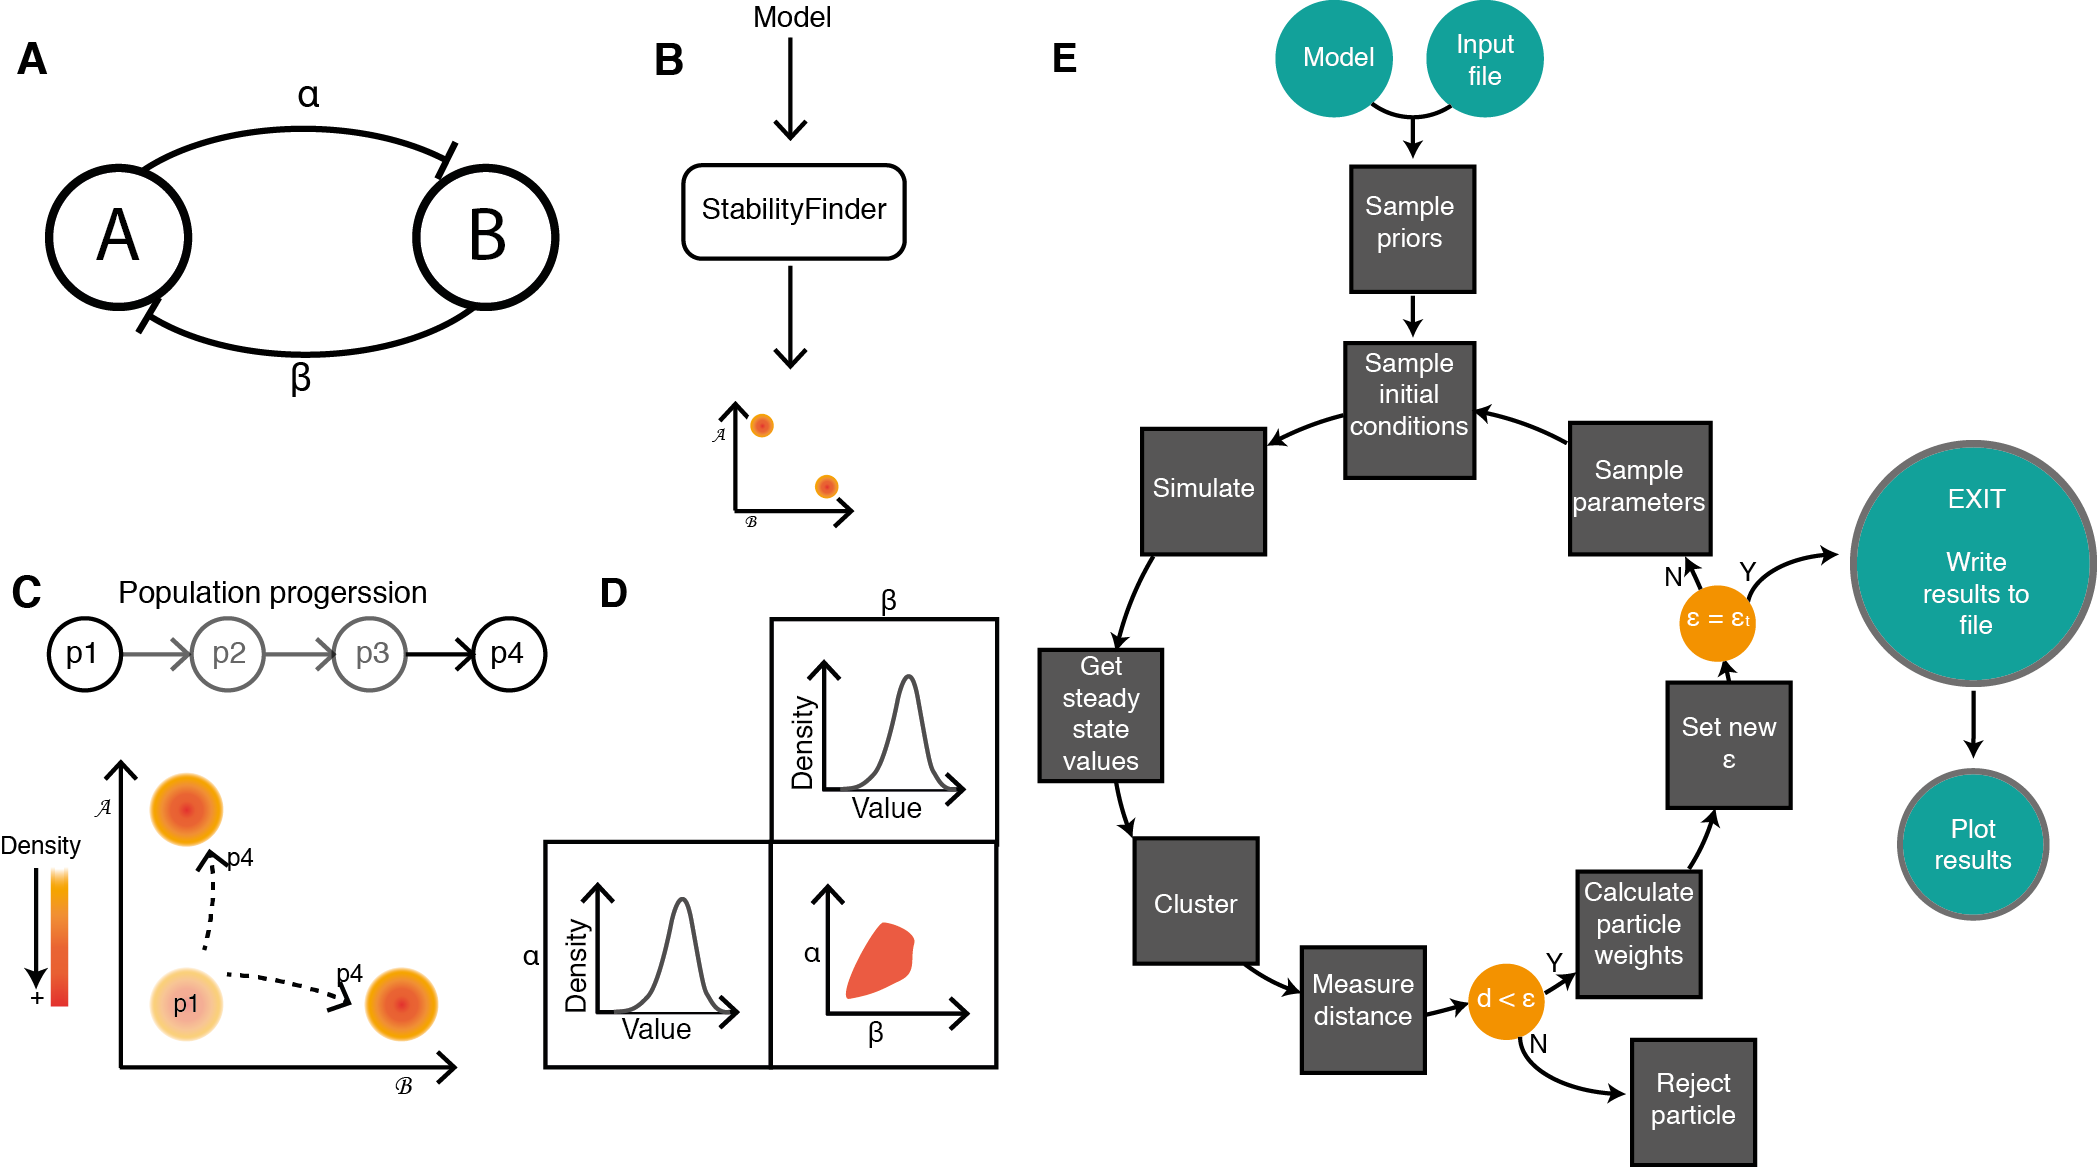
\includegraphics[scale=0.9]{chapterStabilityFinder/images/figure-01.png}
\caption[LoF caption]{\label{fig:fig1}: Using sequential Monte Carlo to examine system stability. The algorithm takes as input a model (A) and evolves it to the stability of choice (C) via intermediate populations. In this example model shown in A, There are two species and two parameters. For the model to be bistable, the phase plot of the two species of interest must have two distinct densities, as shown in (C). The parameter space of the model is searched through our algorithm until the resulting simulations give rise to bistability. The parameter values for the model that demonstrated the desired behaviour are given as an output (D). The output consists of the accepted values for each parameter, as well as each density plotted against the other. This allows us to uncover correlations between parameter values. We made this algorithm into a python package, called StabilityFinder. The overview of the algorithm is shown in (E).}
\end{center}
\end{figure*}
\clearpage

\begin{figure*}[h]
\begin{center}
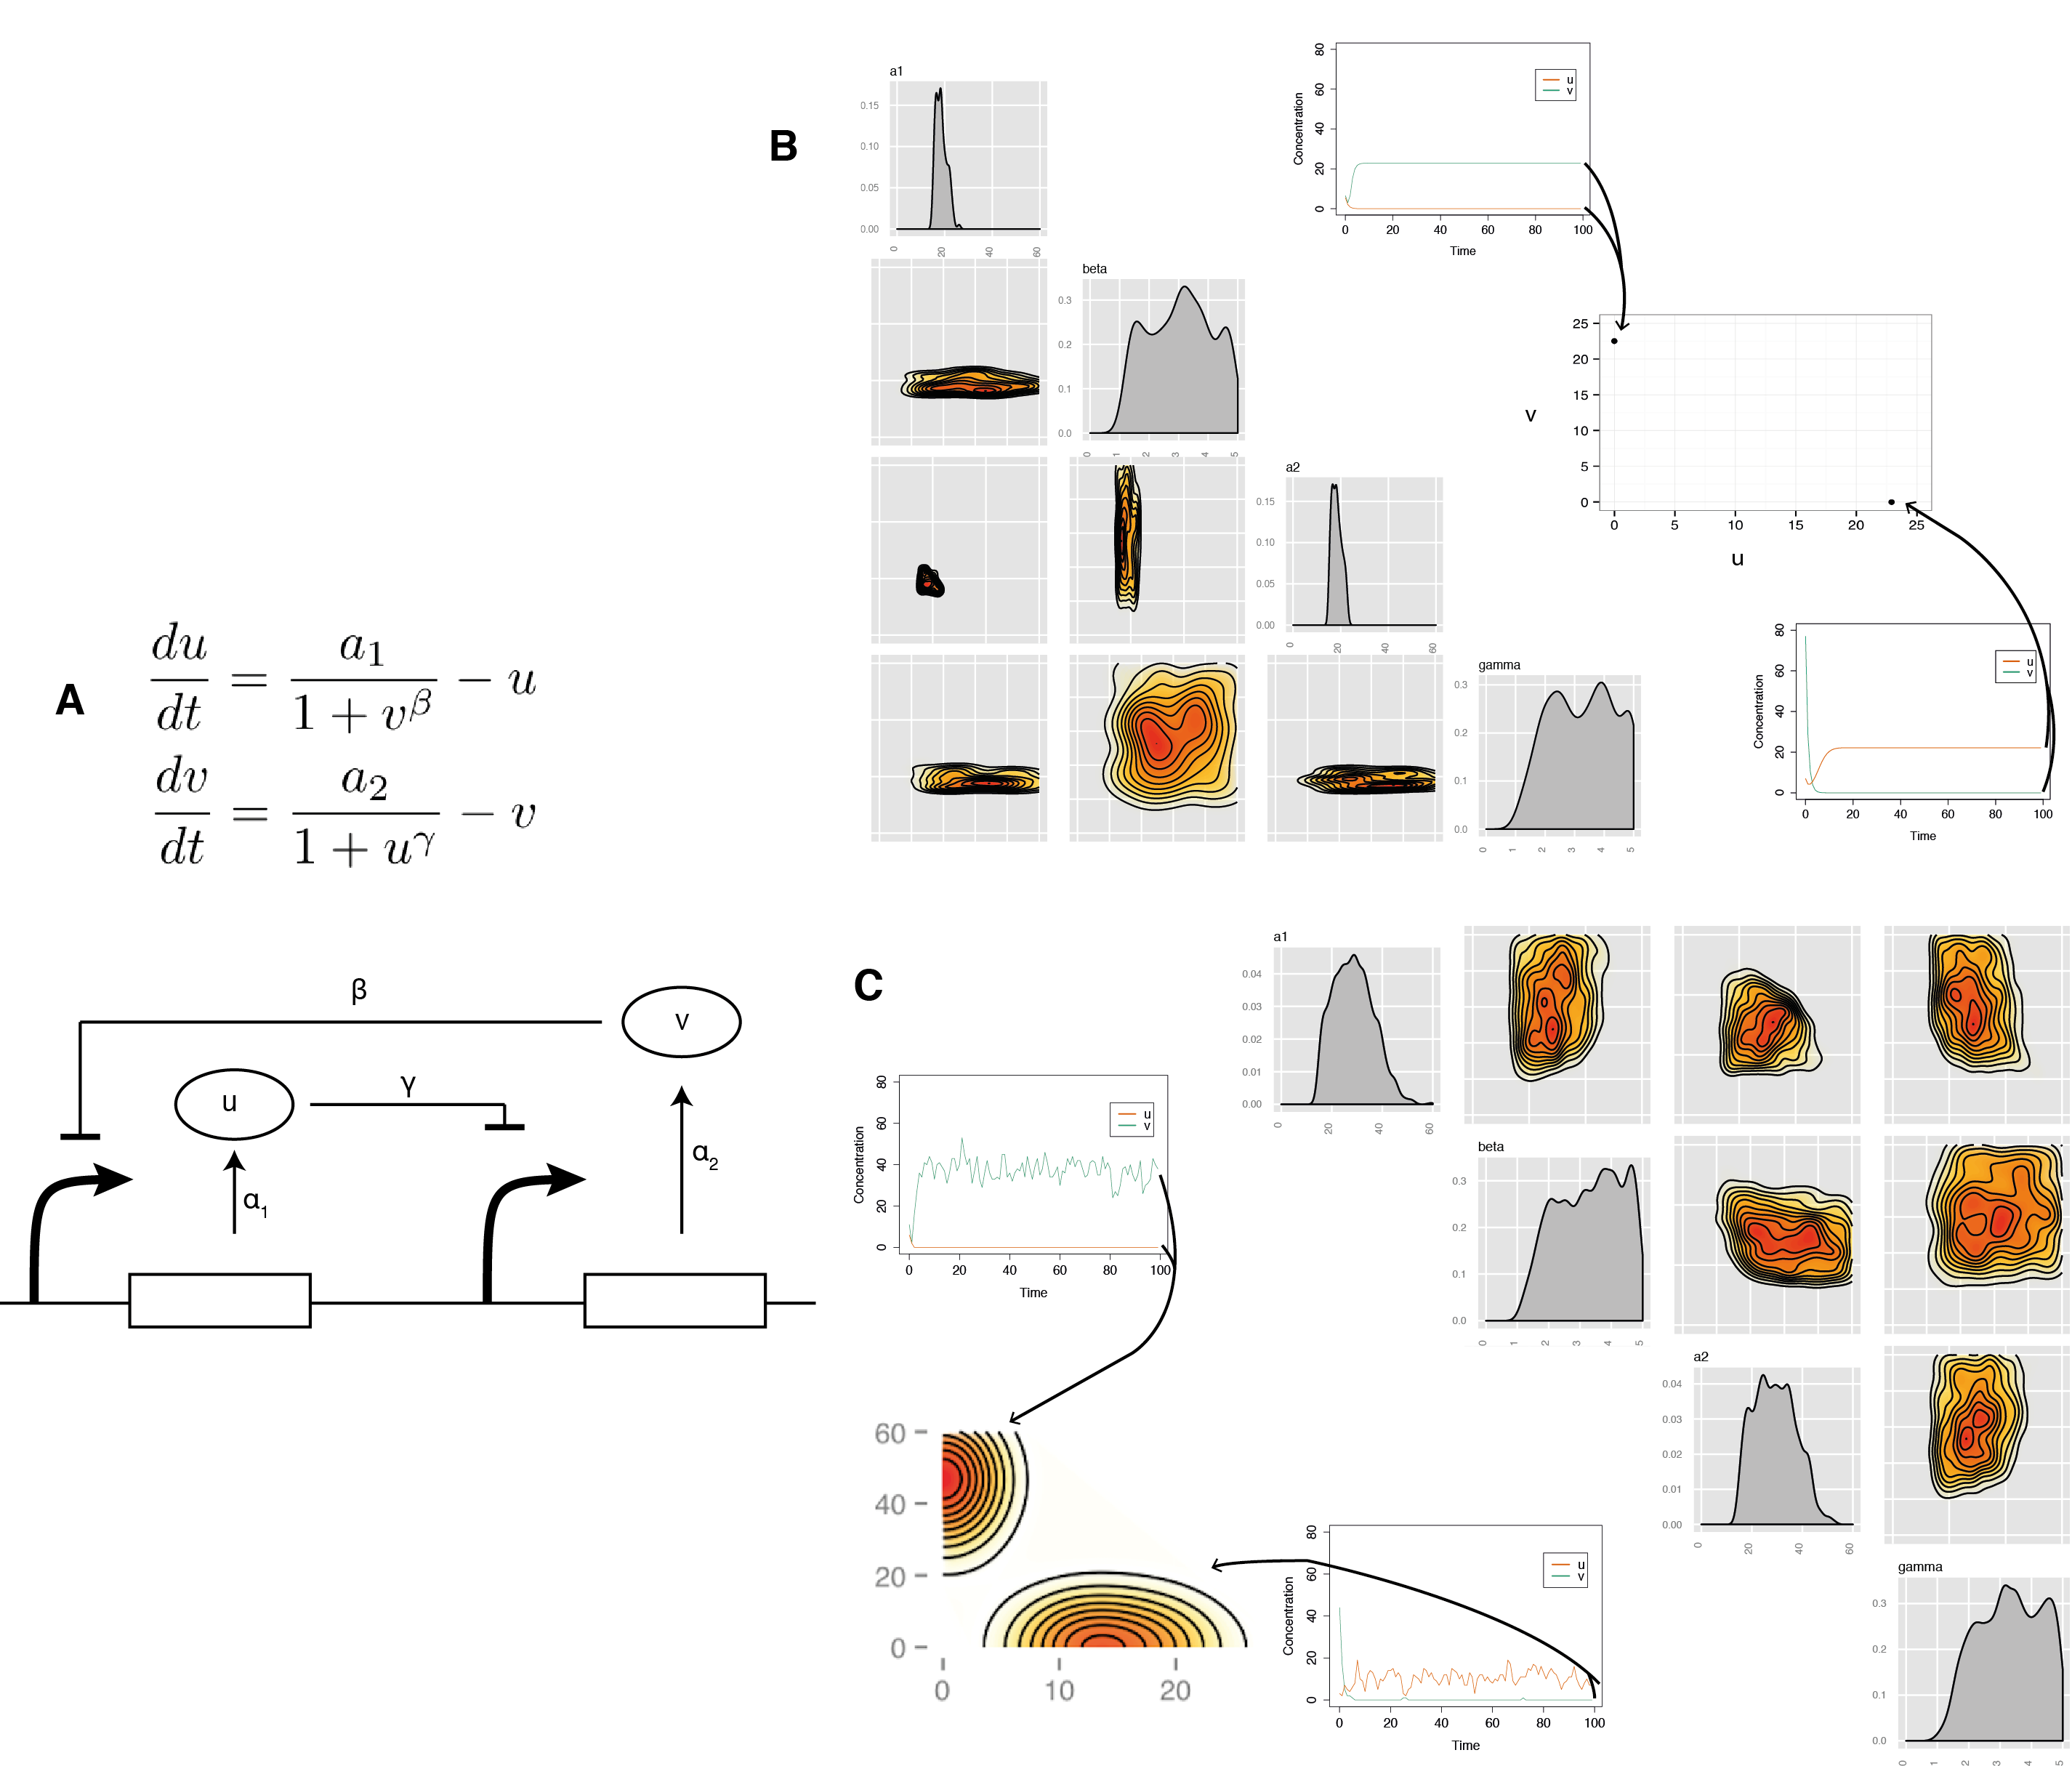
\includegraphics[width=\textwidth]{chapterStabilityFinder/images/figure-02.png}
\caption[LoF caption]{ \label{fig:fig2}: Elucidating the stability of the Gardner switch. The Gardner model (A) consists of two mutually repressing transcription factors. It can be reduced to a two-equation system, where $u$ and $v$ are the two transcription factors, $a_1$,$a_2$ are their effective rates of synthesis, $u$,$v$ are their concentrations and $\beta$, $\gamma$ represent the cooperativity of each promoter. There are four parameters in the model, for which we want to find the values for which this system is bistable. We use StabilityFinder to find the posterior distribution of the bistable Gardner switch, deterministically (B) and stochastically (C). The posterior distributions are shown as the density plots of each parameter as well as each one plotted against the other. }
\end{center}
\end{figure*}
\clearpage

\begin{figure*}[p]
\begin{center}
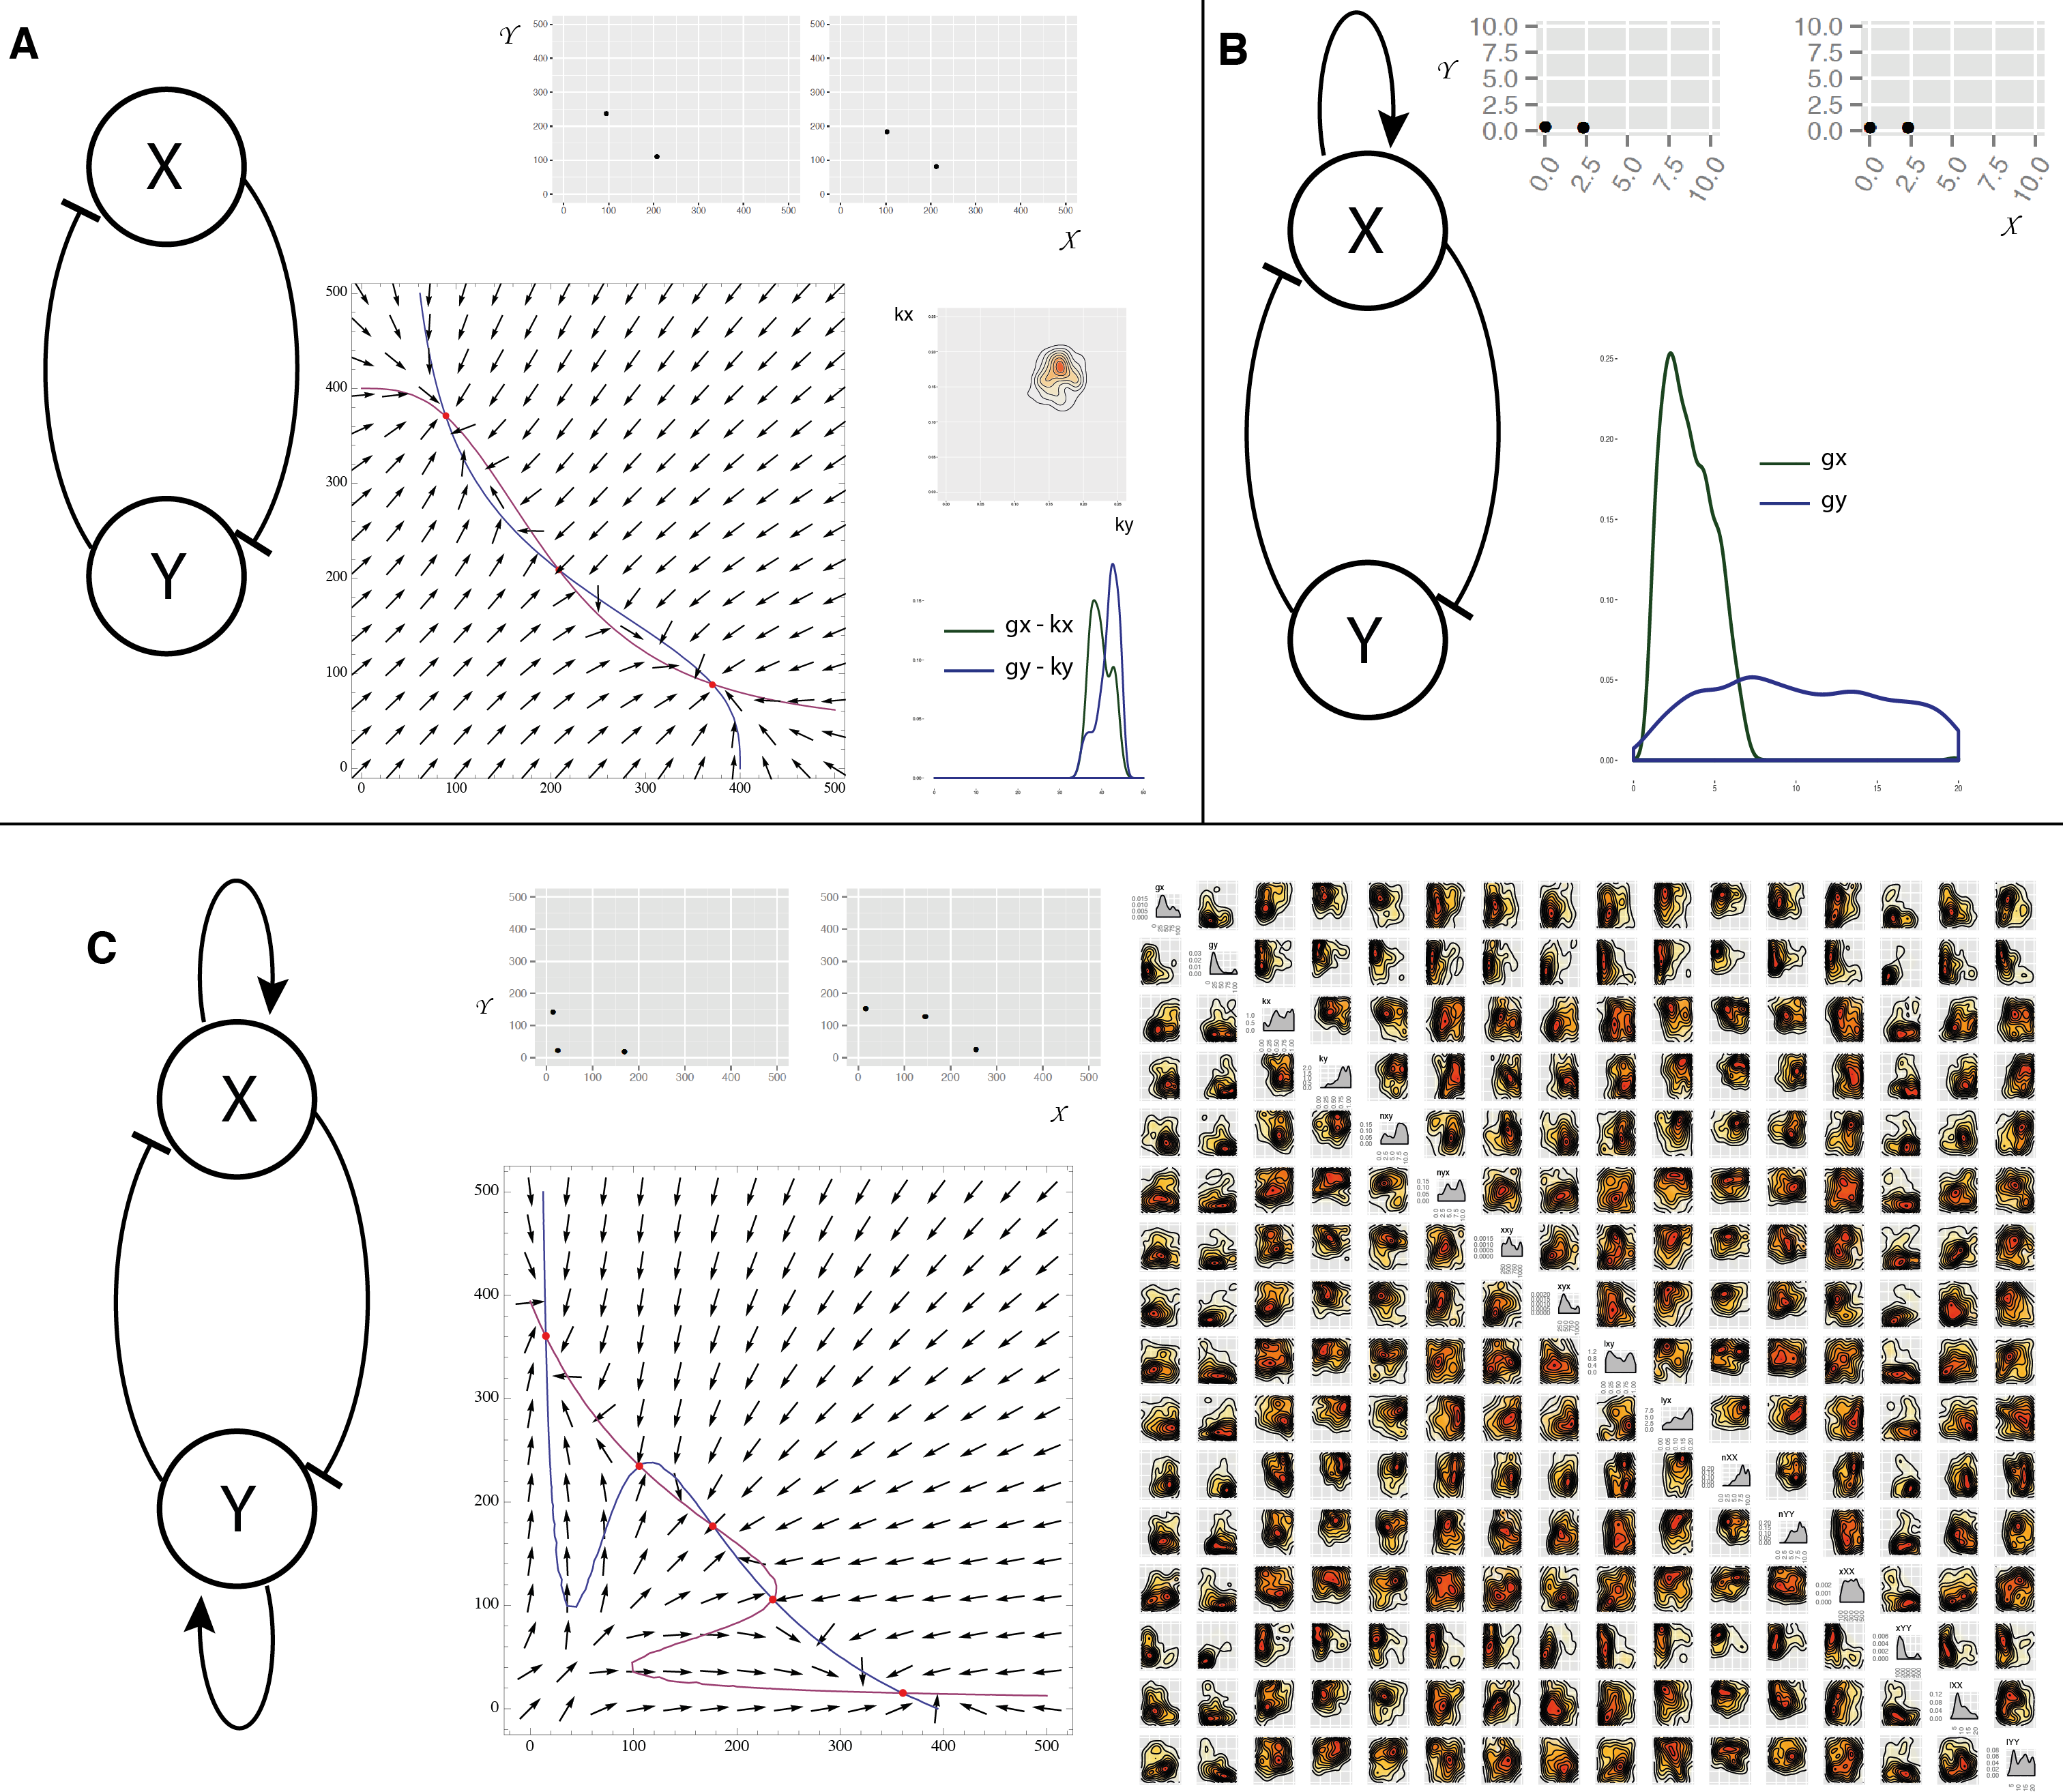
\includegraphics[width=\textwidth]{chapterStabilityFinder/images/figure-03.png}
\caption[LoF caption]{ \label{fig:fig3}: The three variants of the Lu models. (A)\textbf{CS (deterministic).}  The classic switch with no autoregulation is bistable. The most restricted parameters for this behaviour are $kx$ and $ky$ which both have to be high relative to the prior while the net protein production for $X$ and $Y$ myst be balanced. (B)\textbf{SP (deterministic).}The extended Lu model with a single positive autoregulation on $X$. This model is bistable when $gx$ is small. (C) \textbf{DP (deterministic).} The Lu model with double positive autoregulaiton is tristable, and its posterior distribution shown here. We find two types of tristable behaviour, one where the third steady state is zero-zero and one where the third state is high (non-dead).}
\end{center}
\end{figure*}
\clearpage

\begin{figure*}[h]
\begin{center}
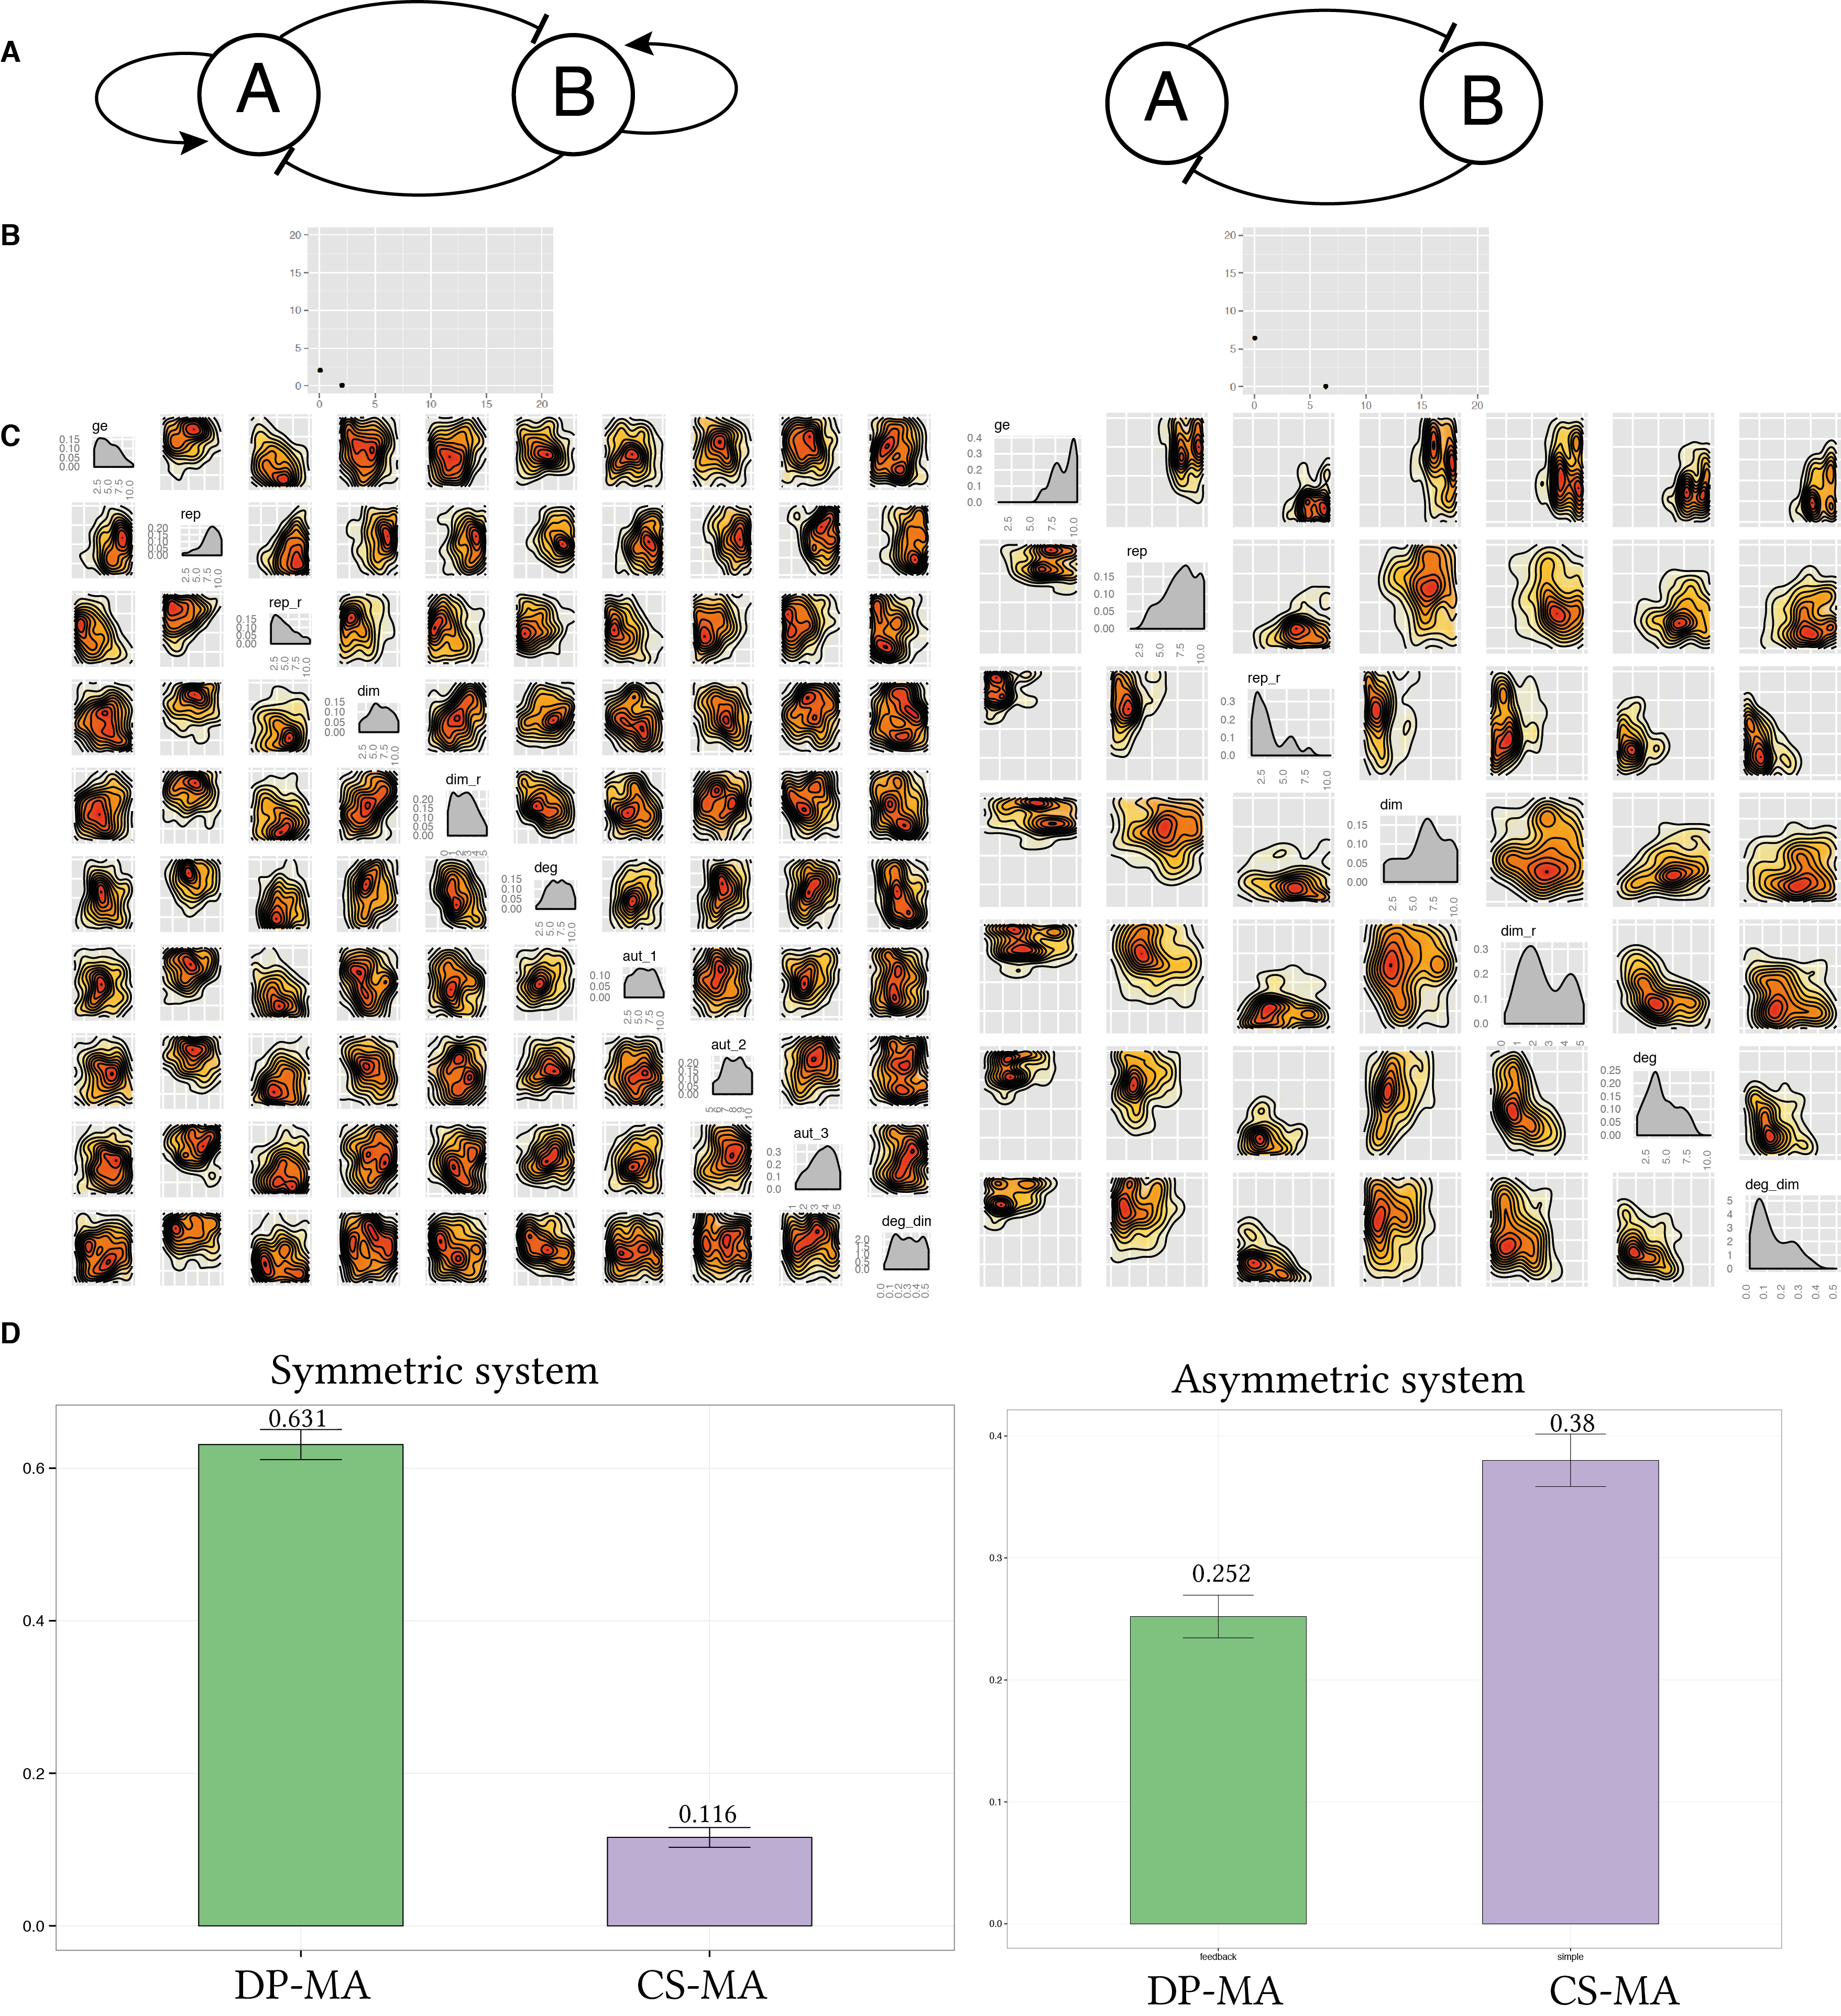
\includegraphics[scale=0.5]{chapterStabilityFinder/images/figure-04.png}
\caption[LoF caption]{ \label{fig:fig4}: Adding positive feedback increases robustness to parameter fluctuations. We compare the posterior distributions of the simple mass action switch and the switch with added double positive autoregulation (A). The two models were both capable of bistable behaviour (B). The two posterior distributions are shown in (C). Comparing the functional region $F$ of the posterior distributions (D) we find that there is a five-fold increase in robustness when positive autoregulation is added. This is not the case for the asymmetric switch in which there is no significant difference in robustness between the CS-MA and DP-MA models.}
\end{center}
\end{figure*}
\clearpage


\begin{figure*}[h]
\begin{center}
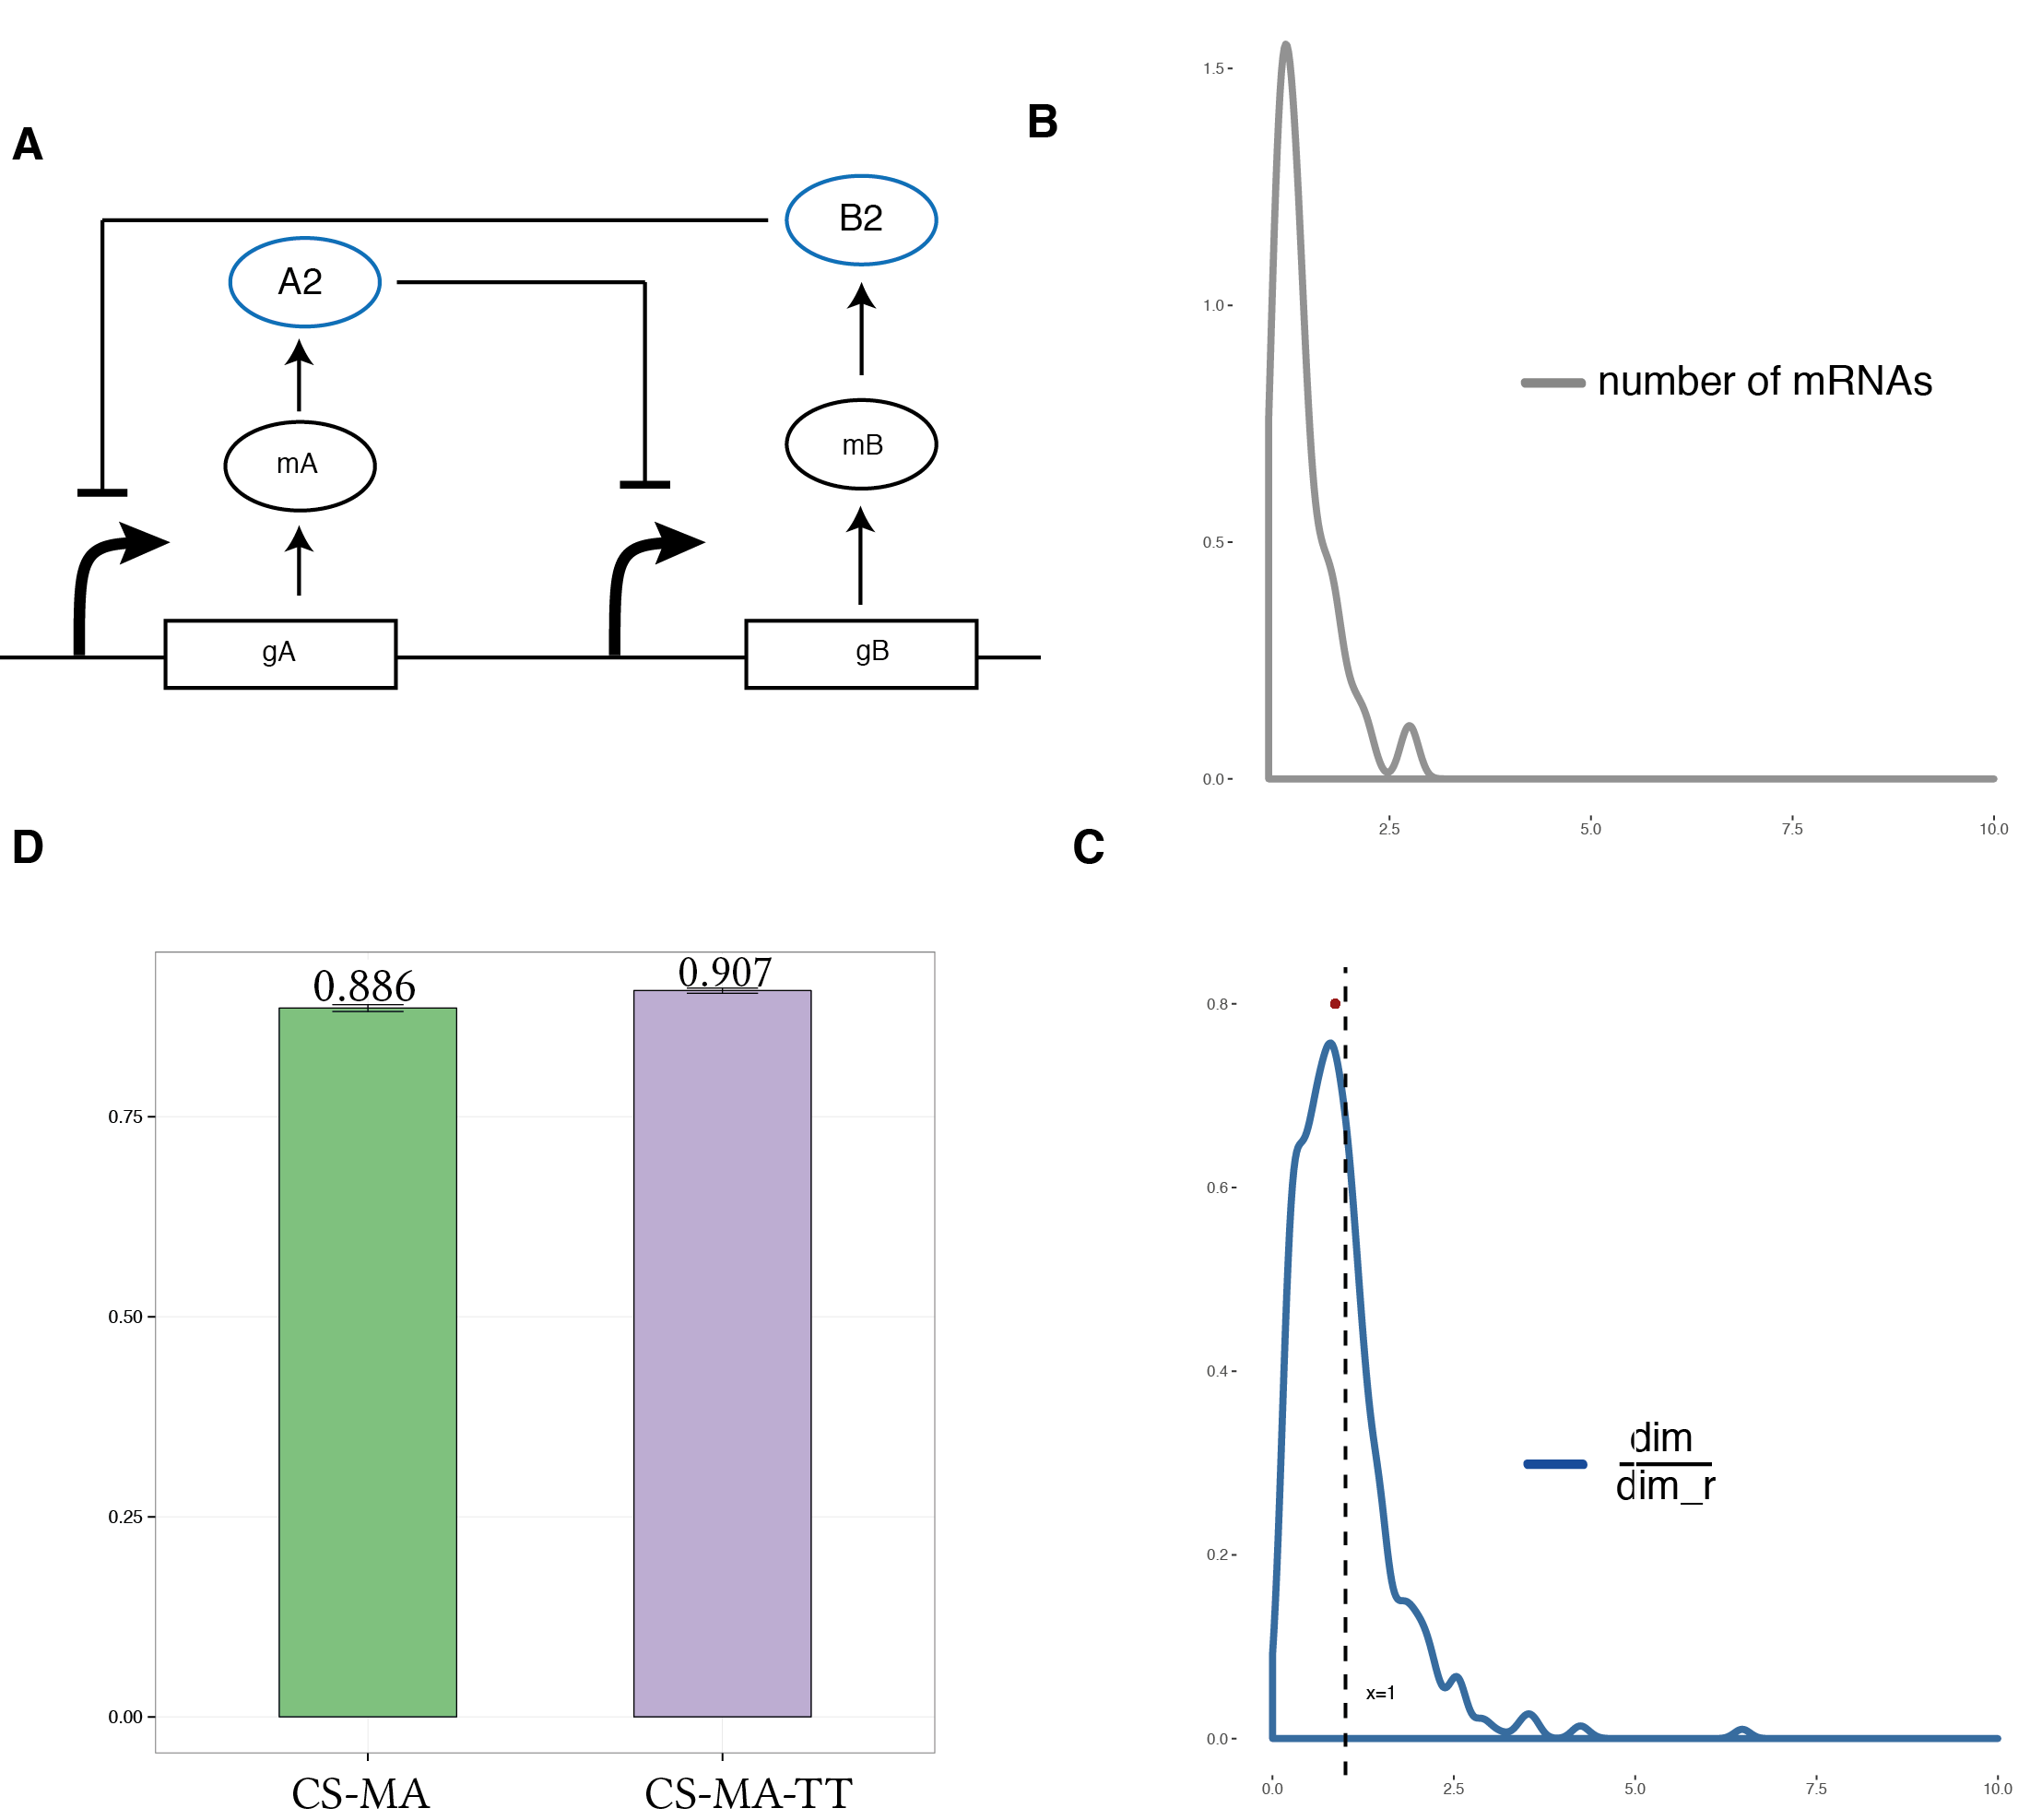
\includegraphics[scale=0.6]{chapterStabilityFinder/images/figure-05.png}
\caption[LoF caption]{ \label{fig:fig5}: (A) Separating transcription and translation in the mass action model. (B) Transcriptional bursting does not allow for a bistable switch. (C) The Quassi Steady state approximation assumption that the dimerization reaction ($dim$) is much faster than its reverse ($dim\_r$) cannot be justified here. The median of the data (red) lies below the x=1 line (black dashed line) which indicates that in the majority of the particles in the posterior $\frac{dim}{dim\_r} < 1$  (D) No difference was found in the robustness to parameter fluctuations for the two models tested here.}
\end{center}
\end{figure*}

\begin{figure*}[h]
\begin{center}
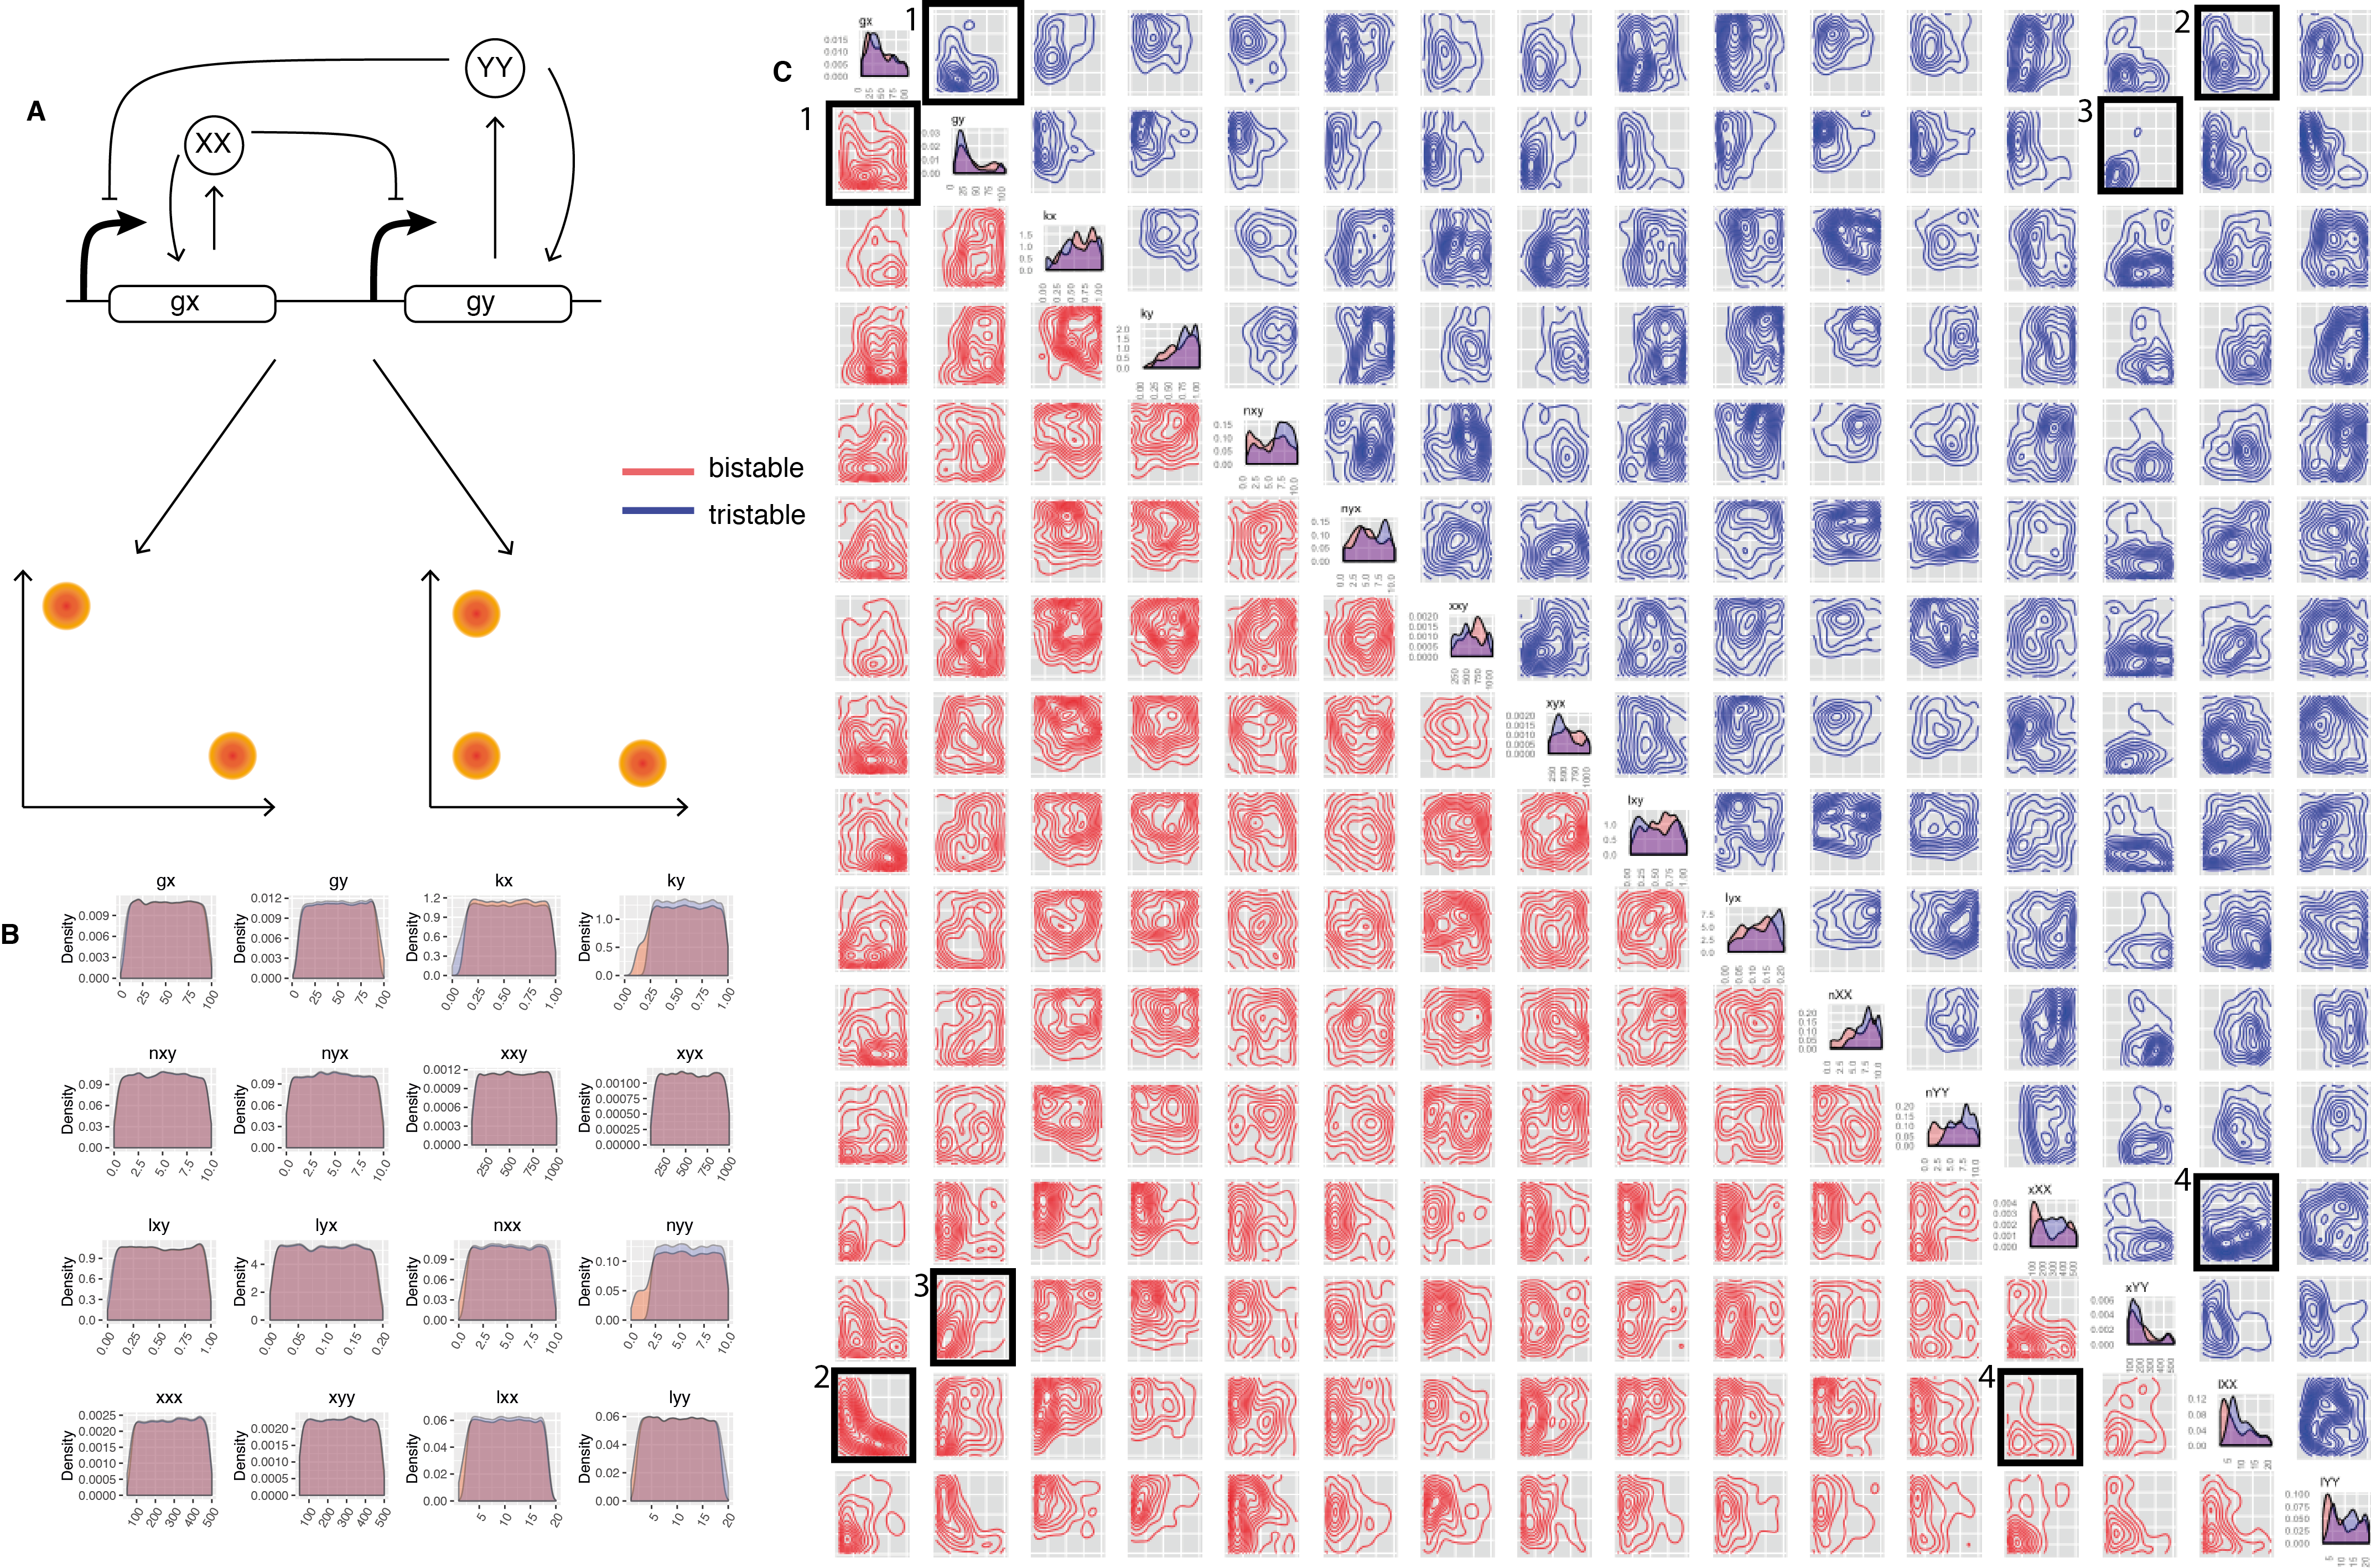
\includegraphics[width=\textwidth]{chapterStabilityFinder/images/figure-06-alt.png}
\caption[LoF caption]{ \label{fig:fig6}: Design principles of a tristable switch. (A) Using the Lu model with added positive autoregulation we uncover the design principles dictating if a switch will be bistable or tristable. (B) By considering each parameter separately we cannot find a significant difference in the parameter values acceptable for a bistable versus a tristable switch. (C) By considering the bivariate distributions of the parameters we can uncover the differences in the parameters of a bistable switch compared to a tristable switch. The posterior distribution of the bistable switch is shown in red and of the tristable switch in blue. The bivariate distributions for which a difference is observed between a bistable and a tristable switch are in black boxes. }
\end{center}
\end{figure*}


\begin{figure*}[h]
\begin{center}
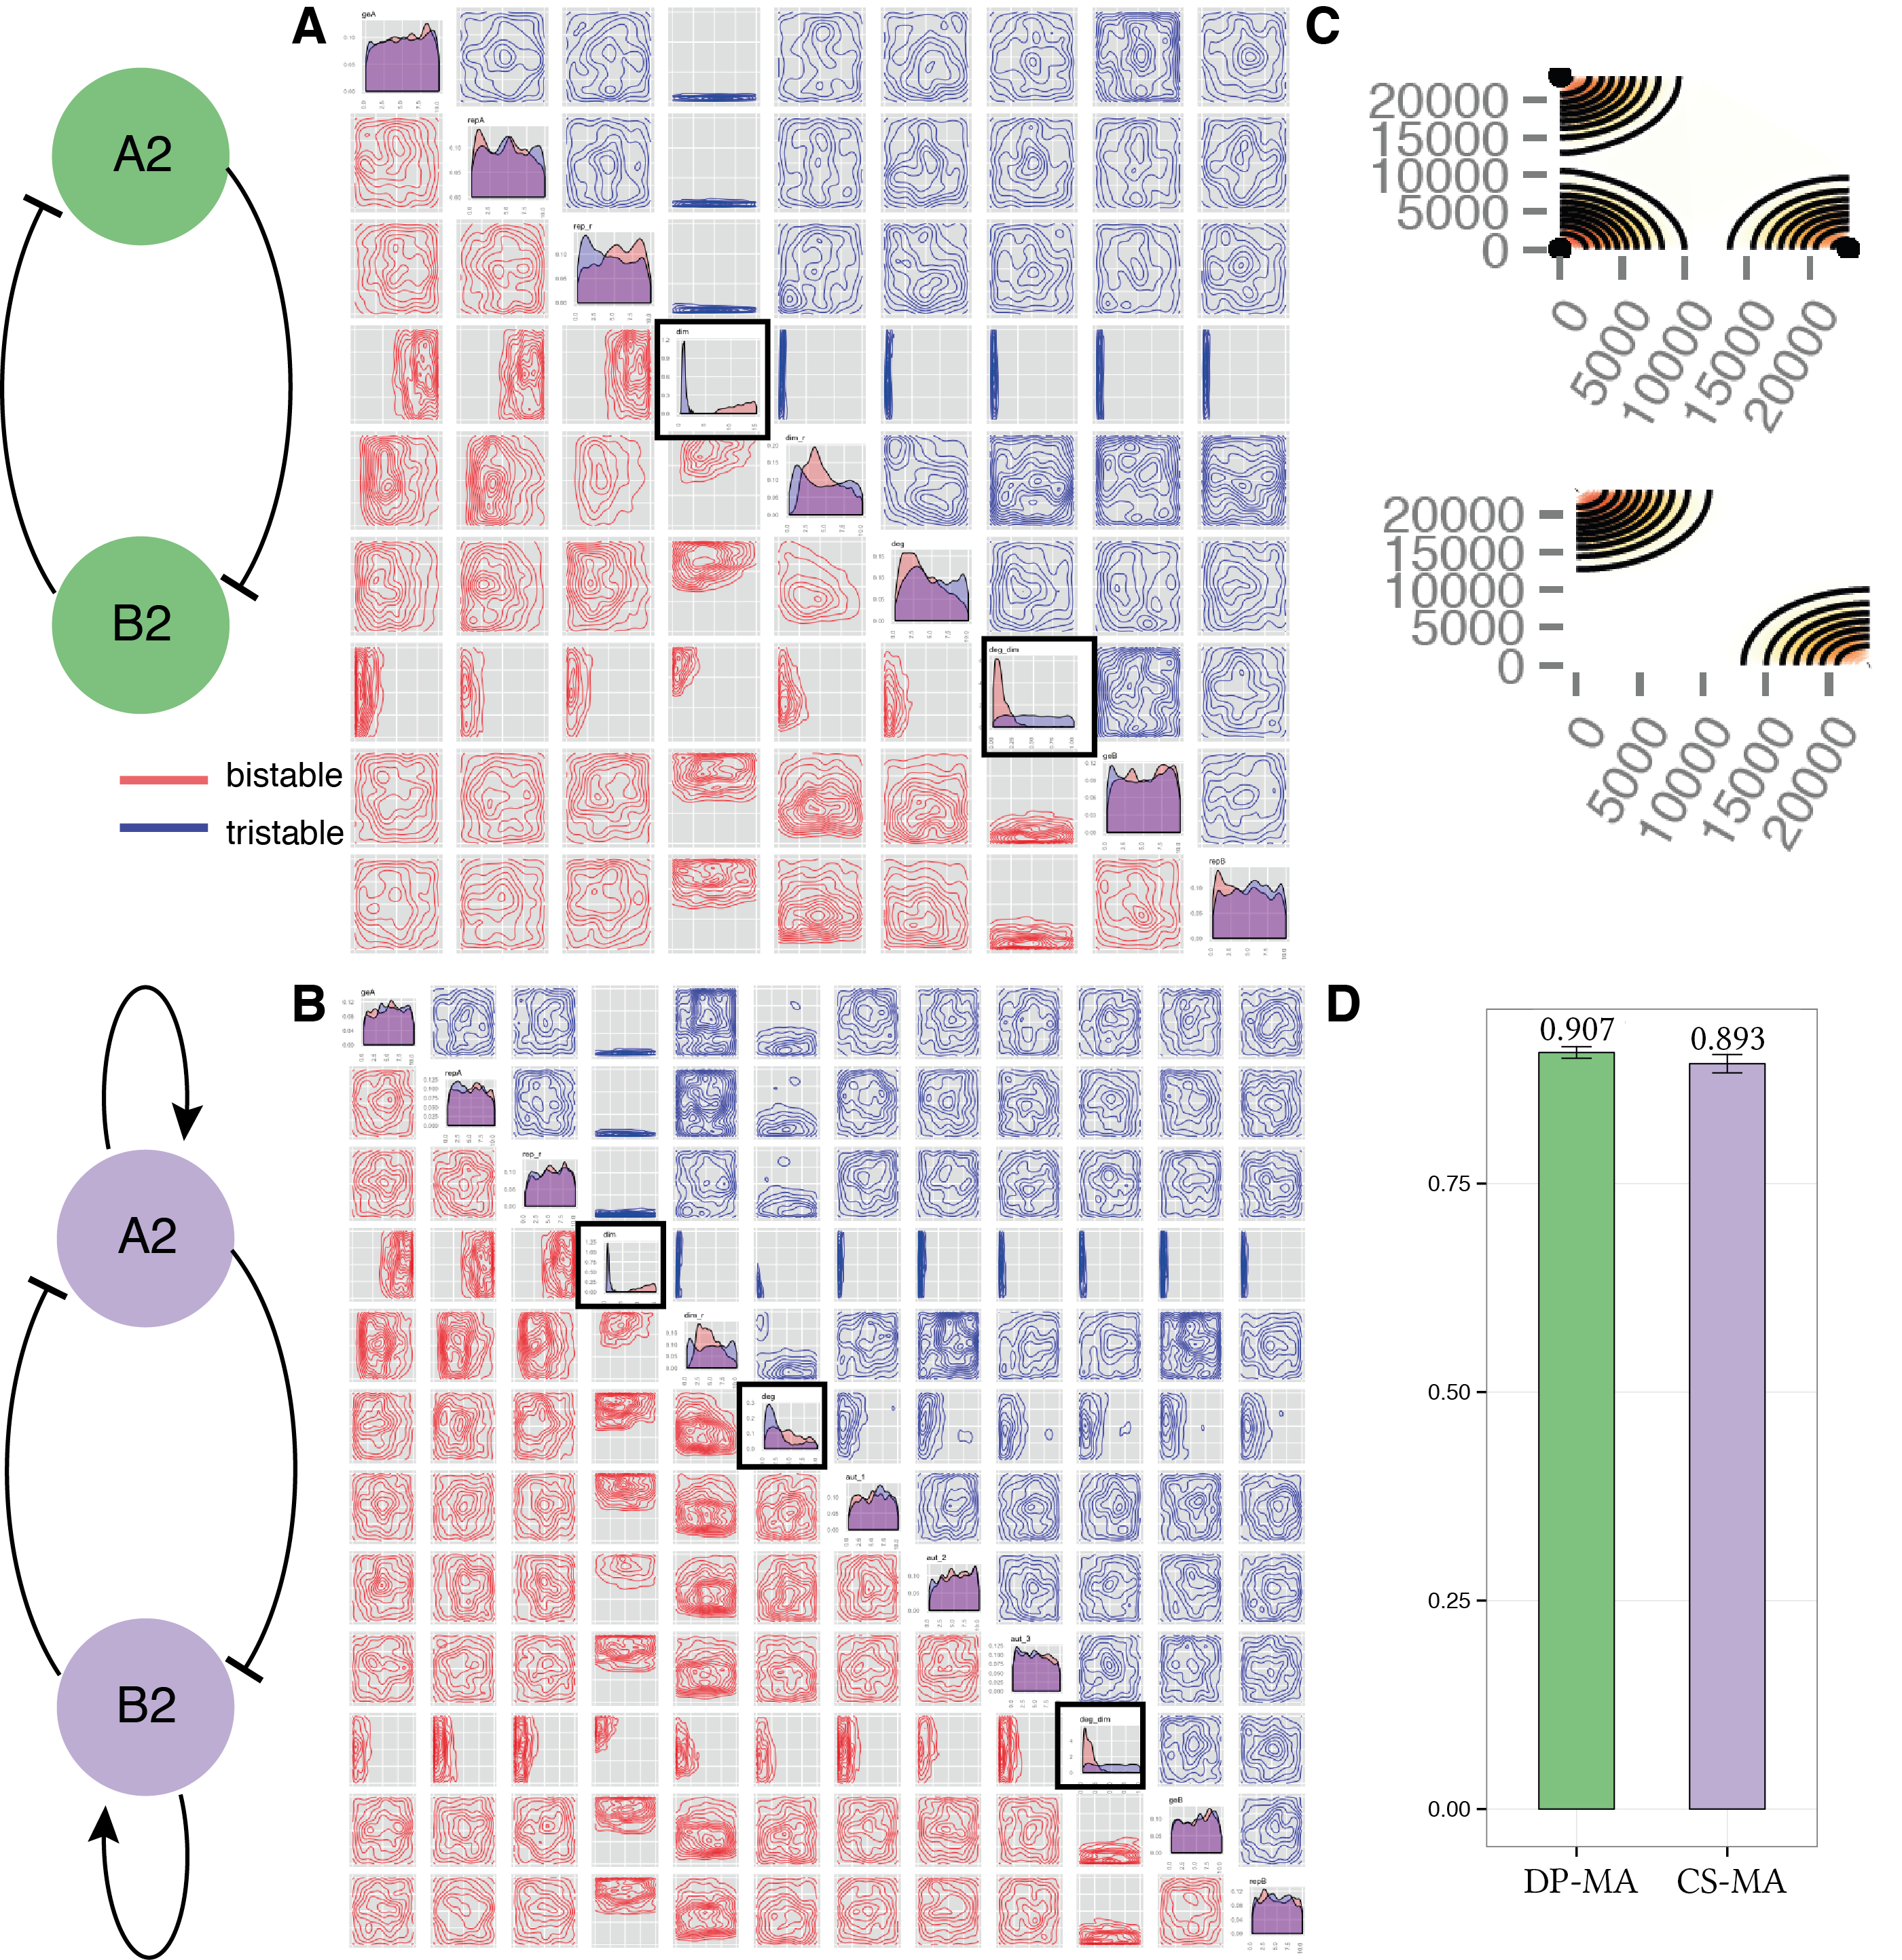
\includegraphics[scale=0.6]{chapterStabilityFinder/images/figure-07.png}
\caption[LoF caption]{ \label{fig:fig7}: Tristability is possible in the mass action toggle switch models only when simulated stochastically. (A) the simple toggle switch with no autoregulation can be both bistable and tristable. The two posteriors are shown, where the posterior distribution of the bistable switch is shown in red and of the tristable switch in blue. From the posterior distribution we can deduce the the dimerization parameter must be small for tristability to occur but large for bistability. The switch with double positive autoregulation and its posterior distributions for the bistable and tristable case are shown in (B). A sample phase plot of a stochastic tristable and bistable mass action switch is shown in (C). Comparing the robustness of the switch with and without positive autoregulation, we don't find a significant difference (D).}
\end{center}
\end{figure*}
\clearpage

\begin{figure*}[h]
\begin{center}
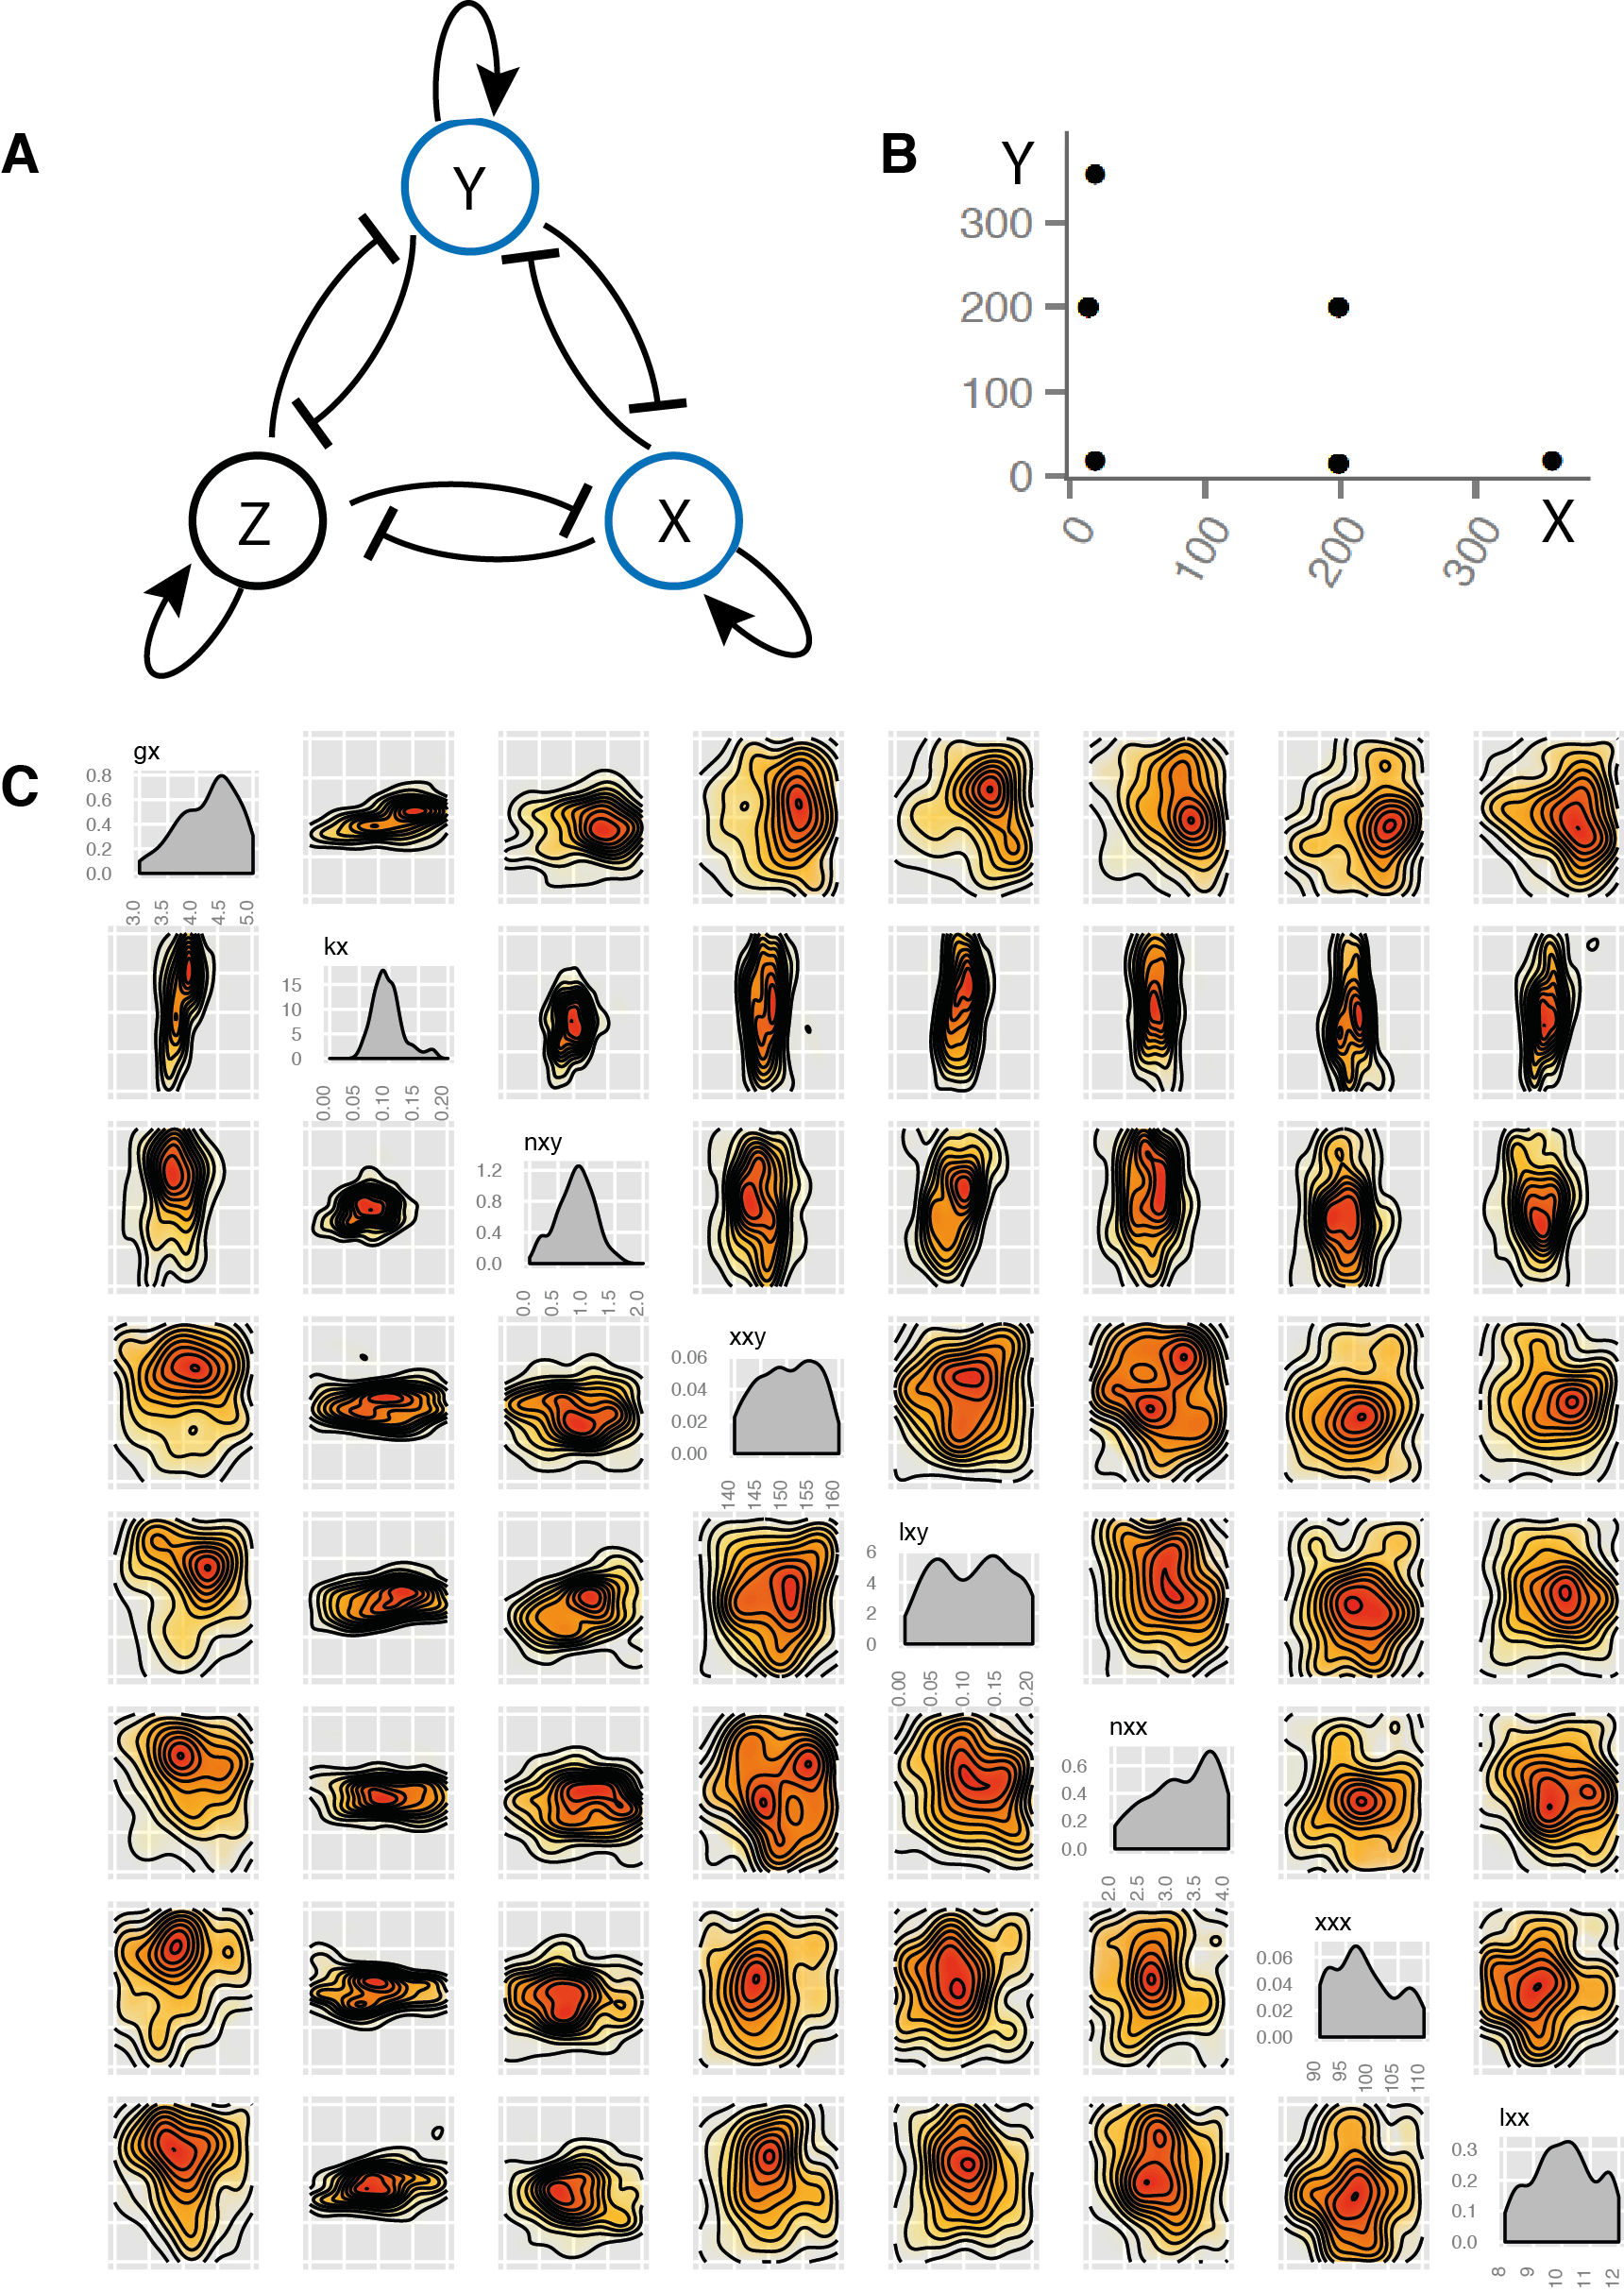
\includegraphics[scale=0.7]{chapterStabilityFinder/images/figure-08.png}
\caption[LoF caption]{ \label{fig:fig8}: The three-node mutual repression model, with added positive auto-regulation on each node. (A) The model. The model is studied in two dimensions using StabilityFinder, $X$ and $Y$. (B) The phase plot of the resulting final population of StabilityFinder. There are 6 steady states. (C) The posterior distribution of the 6-steady state three-node system. Parameters $kx$ and $nxy$ are the most constrained.}
\end{center}
\end{figure*}


%\section{Methods}

 
 
\subsection{Calculating robustness}




%\section{Results}
\subsection{Testing StabilityFinder: The Gardner toggle switch}

This toggle switch model was developed by T.~S. Gardner~\autocite{Gardner:2000vha}. This model consists of two mutually repressing transcription factors and is defined by the following ODEs:

\begin{align}
\frac{du}{dt} &= \frac{a_1}{1+v^{\beta}} - u \label{eq:gard_1} \\
\frac{dv}{dt} &= \frac{a_2}{1+u^{\gamma }} - v\label{eq:gard_2}
\end{align}
Where $a_1$ and $a_2$ are the effective rates of synthesis of repressors 1 and 2 respectively. \textit{u} is the concentration of repressor 1 and \textit{v} the concentration of repressor 2. \textit{$\beta$} is the cooperativity of repression of promoter 1 and \textit{$\gamma$} of repressor 2. In their paper,  T.~S. Gardner~\autocite{Gardner:2000vha} state that there are two conditions for bistability of this toggle switch model. That $a_1$ and $a_2$ are balanced and that $\beta$ and $\gamma$ are \textgreater 1. In order to test our methodology, we used StabilityFinder to find the posterior distribution for which this model exhibits bistable behaviour. So setting the desired behaviour to bistable, and using for priors a wide range of values that includes the values used in the Gardner paper, we test StabilityFinder to see if it finds the same conditions as the ones set by T.~S. Gardner. The prior distributions used are shown in Table~\ref{tab:gard}. The posterior distribution calculated by StabilityFinder is shown in Figure~\ref{fig:Gard_post}.

\cleardoublepage
\begin{figure}[t]
\centering
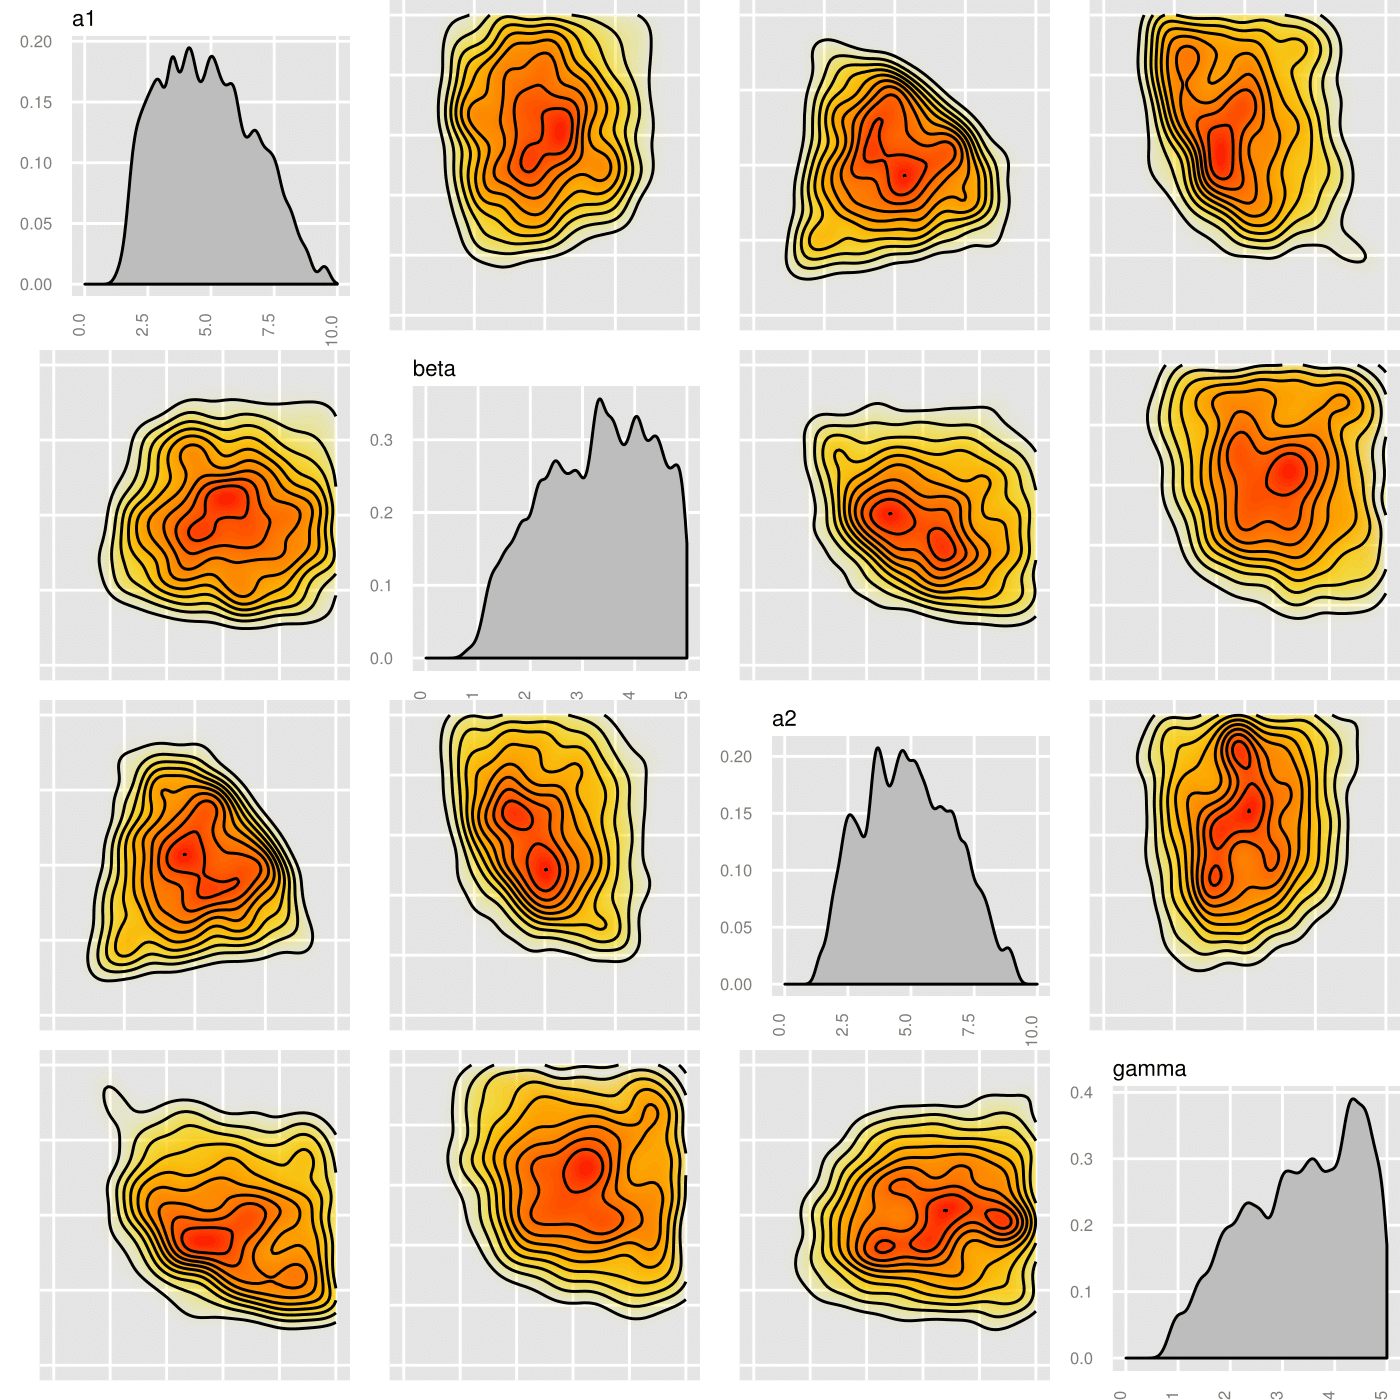
\includegraphics[scale=0.2]{chapterStabilityFinder/images/Gardner/posterior.png}
\caption[The posterior distribution of the bistable Gardner toggle switch]{The posterior distribution of the bistable Gardner toggle switch. The parameters $a_1$, $a_2$ represent to the effective synthesis rate of repressors 1 and 2 respectively. Parameters $\beta$, $\gamma$ represent the cooperativity on repressors 1 and 2 respectively. The marginal distributions of each parameter are found on the diagonal and pairwise joint distributions along the sides.}
\label{fig:Gard_post}
\end{figure}


\begin{figure}[t]
\centering
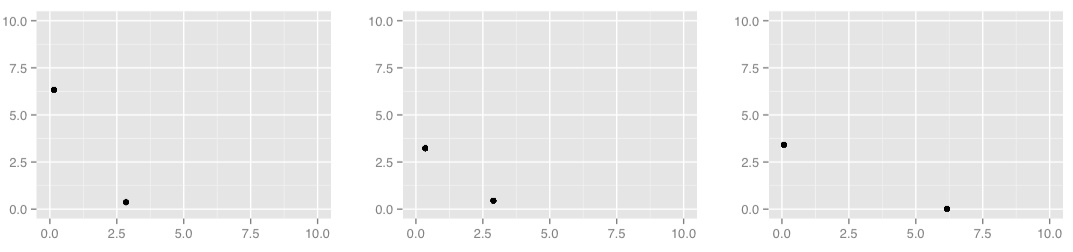
\includegraphics[scale=0.3]{chapterStabilityFinder/images/Gardner/phase_plots.png}
\caption{A sample of the phase plots produced from the final population of the Gardner switch.}
\label{fig:det_gard_phase}
\end{figure}

\begin{table}[b]
\centering
\caption{Gardner switch priors}
\label{tab:gard}
\begin{tabular}{cccc|cc}
\multicolumn{4}{c|}{Parameters} & \multicolumn{2}{c}{Species} \\ %\hline
$a_1$   & $\beta$   & $a_2$   & $\gamma$  &   $s_1$      &       $s_2$   \\
0-10    & 0-5       & 0-10    &  0-5      &      0-100   &          0-100   
\end{tabular}
\end{table}

These results agree with the results reported by the original paper~\autocite{Gardner:2000vha} . For this switch to be bistable $a_1$ and $a_2$ must be balanced while $\beta$ and $\gamma$ must both be \textgreater 1, as can be seen in the marginal distributions of $\beta$ and $\gamma$ in Figure~\ref{fig:Gard_post}. The conditions set by the original paper for parameters $a_1$ and $a_2$ are met, as the joint distribution shown in Figure~\ref{fig:Gard_post} matches the bifurcation lines calculated in the original paper. 
This successful test demonstrates that StabilityFinder can be used to find the stability a model is capable of as well as the parameter ranges that can produce that. This allows us to confidently apply the methodology to further models.
%-%-%-%-%-%-%%-%-%-%-%-%-%%-%-%-%-%-%-%

\subsubsection{Comparing the deterministic and stochastic cases} 
    
There are two main ways of modelling a system, deterministically and stochastically. Deterministic modelling utilises ordinary differential equations (ODE) and models the concentrations of the species (proteins or other molecules) by time-dependent variables~\autocite{deJong:2002ft}. Rate equations are used to model gene regulation where the rate of production of a species is a function of the concentrations of the other species~\autocite{deJong:2002ft}. When modelling deterministically the model is viewed as a system which, with sufficient knowledge of the system, its behaviour is entirely predictable. Nevertheless we are still a long way away from having complete knowledge of a system of interesting size~\autocite{wilkinson:2006}. Deterministic modelling also assumes a homogenous mixture where species concentrations vary continuously and deterministically, assumptions that often are not met \textit{in vivo}. A cell is spatially and temporally separated, due to small molecule numbers and fluctuations in the timing of processes~\autocite{deJong:2002ft}.  
   
In stochastic modelling, species are measured in discrete amounts rather than concentrations and a joint probability distribution is used to express the probability that at time \textit{t} the cell contains a number of molecules of each species~\autocite{deJong:2002ft}. It takes uncertainty into account and is thus often more appropriate for modelling cellular systems, although more computationally intensive. In stochastic systems the Gillespie algorithm is widely used to simulate the time-evolution of the state of the system~\autocite{Warren:2005kea}.

The toggle switch has been modelled both deterministically and stochastically, with the two methods producing different results. Thus here we use StabilityFinder to compare the stabilities that the model is capable of, under the different simulation types. By using the same framework, and the same prior distributions for the models, one can directly compare the posterior distributions produced by the deterministic and the stochastic case, and uncover the effects that are due to the stochasticity of the system. This is relevant in a a biological model in which small molecule numbers and external noise are not negligible. Using StabilityFinder and using the same priors for the two models (Table~\ref{tab:gard_det_stoch}), we calculated the posterior for each both bistable models. The results are shown in Figure~\ref{fig:Gard_summary}. The prior ranges used are much wider than in the test case in order to allow more flexibility in both models and have a greater range over which to compare the models. 


\begin{table}[h]
\centering
\caption{Gardner switch priors in the deterministic and stochastic cases}
\label{tab:gard_det_stoch}
\begin{tabular}{cccc|cc}
\multicolumn{4}{c|}{Parameters} & \multicolumn{2}{c}{Species} \\ %\hline
$a_1$   & $\beta$   & $a_2$   & $\gamma$  &   $s_1$      &       $s_2$   \\
0-60    & 0-5       & 0-60    &  0-5      &      0-100   &          0-100   
\end{tabular}
\end{table}

\begin{figure}[p]
\centering
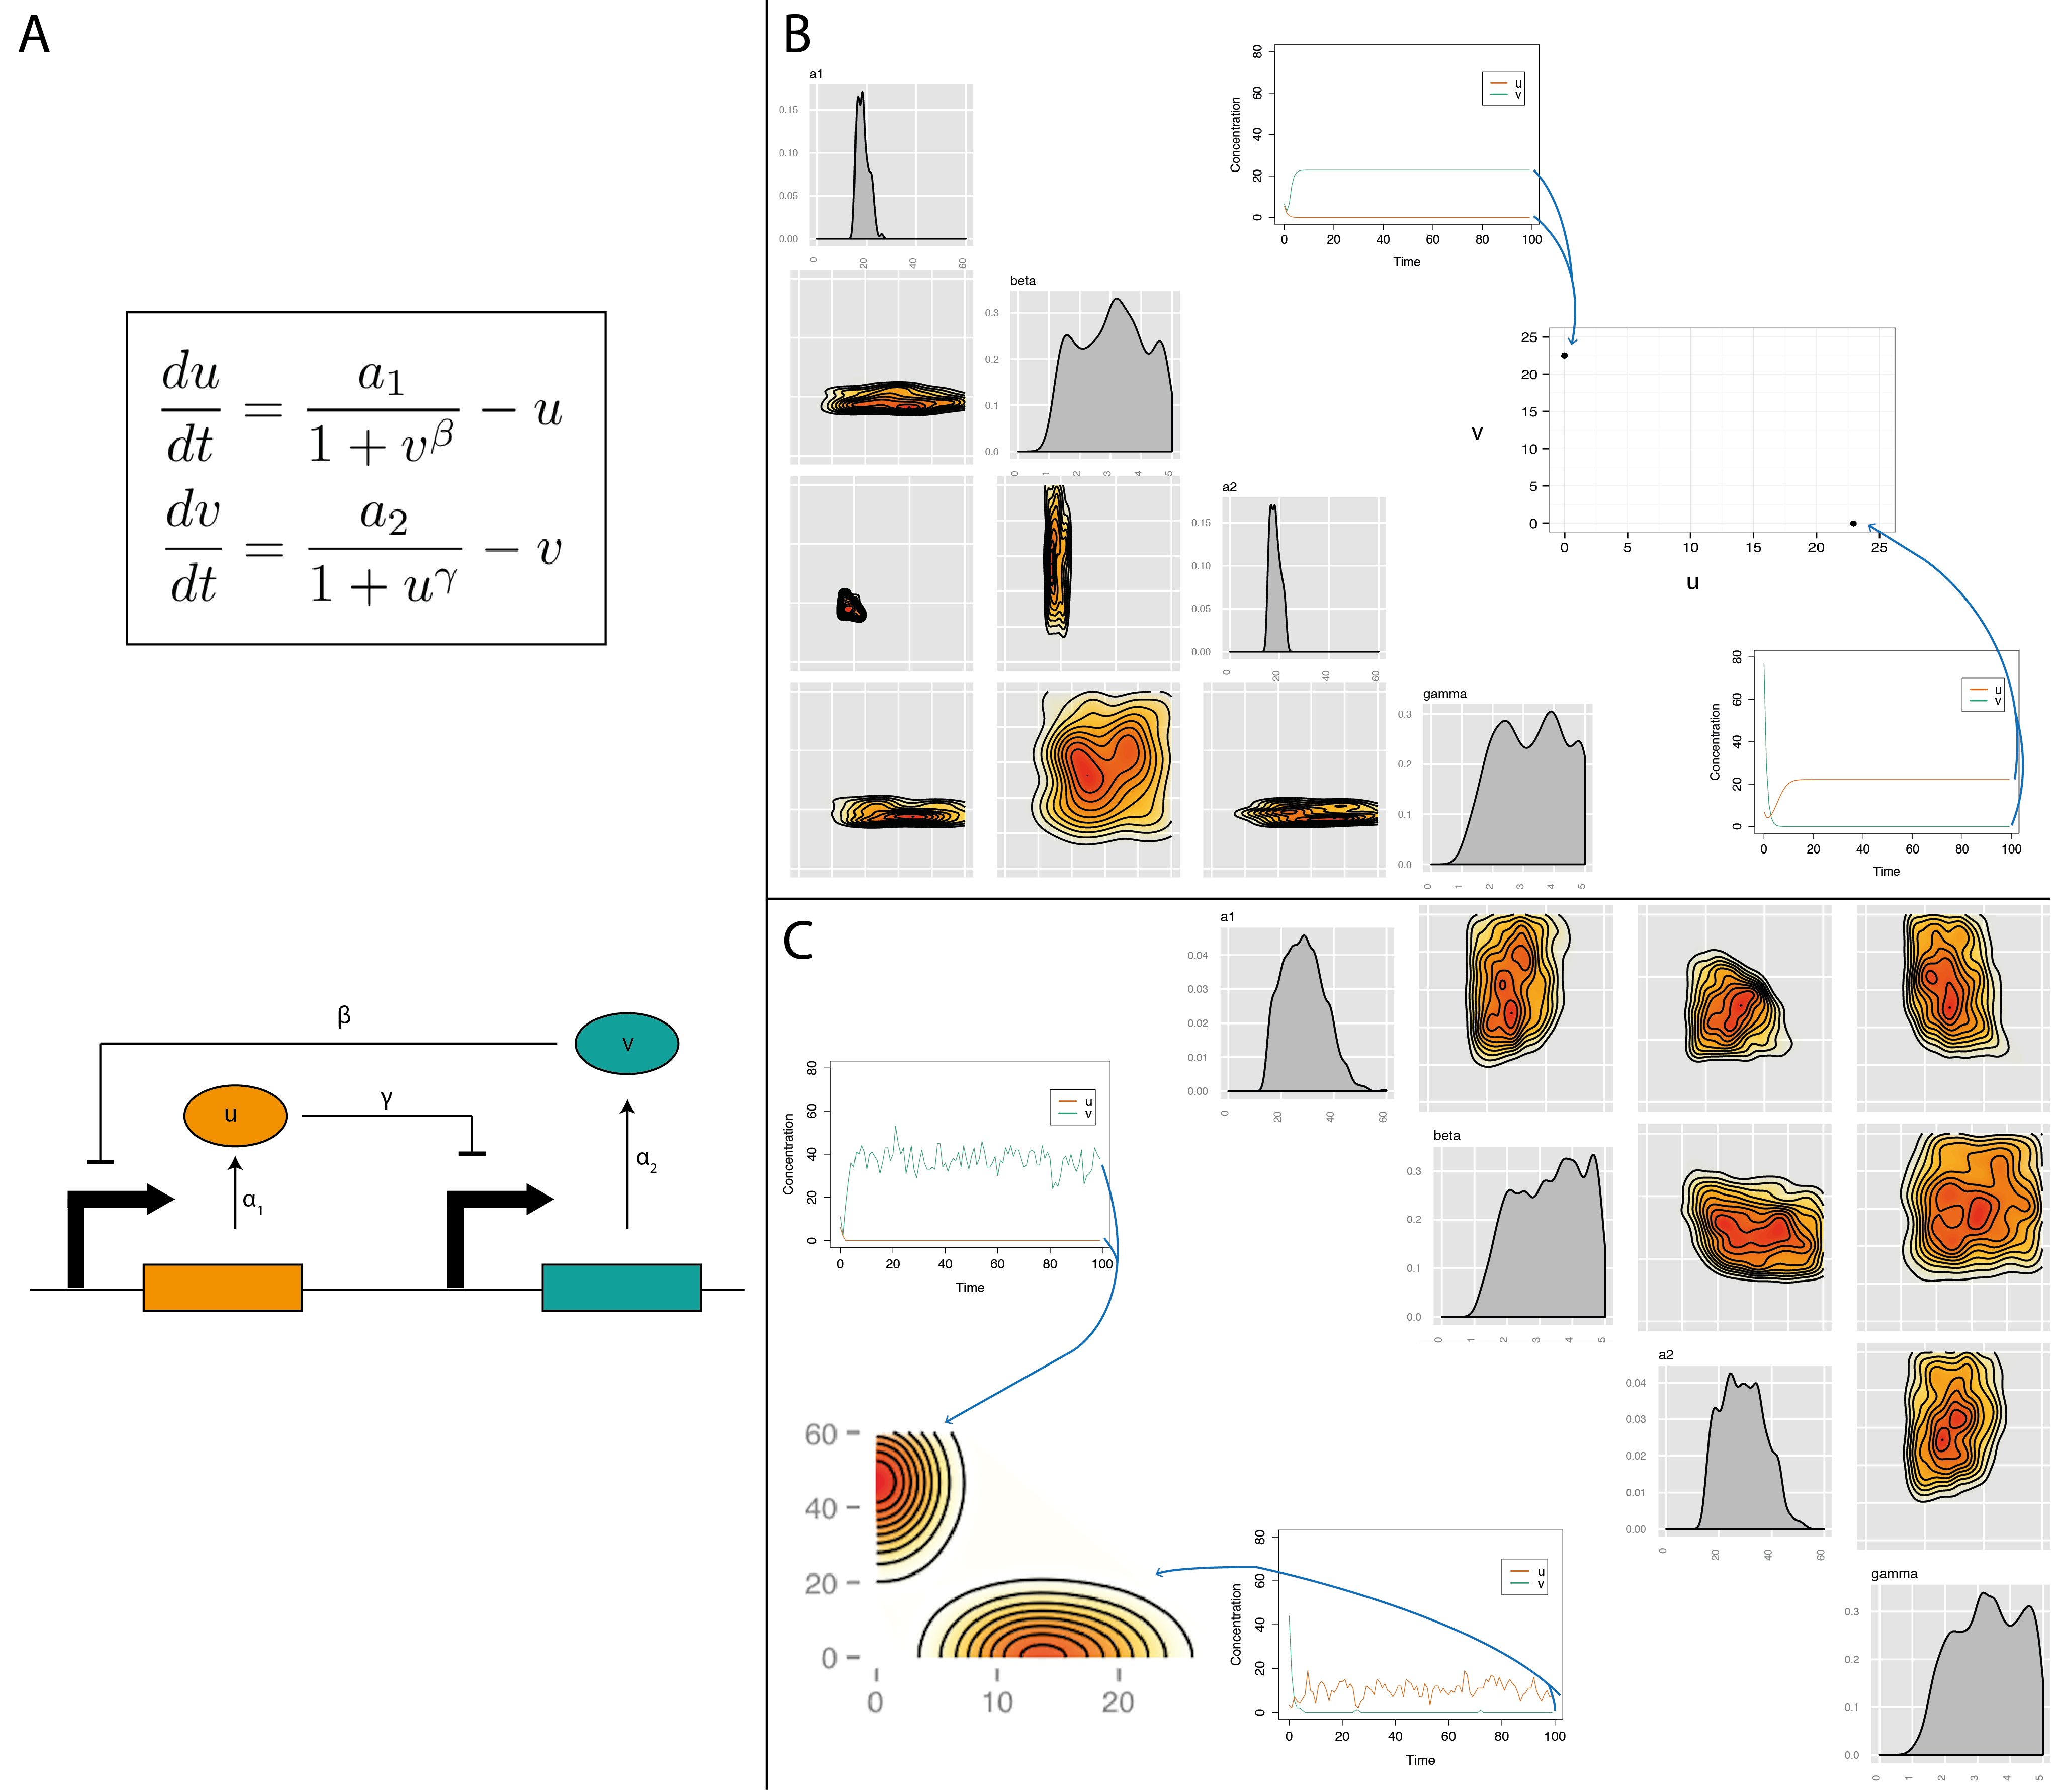
\includegraphics[scale=0.45]{chapterStabilityFinder/images/Gardner/summary.png}
\caption[The stochastic and deterministic cases of the Gardner toggle switch]{The Gardner toggle switch is modelled stochastically and deterministically. The model is shown graphically and mathematically in (A), The posterior and phase space of the deterministic model is shown in (B) and of the stochastic case in (C).}
\label{fig:Gard_summary}
\end{figure}


%\begin{figure}[p]
%\centering
%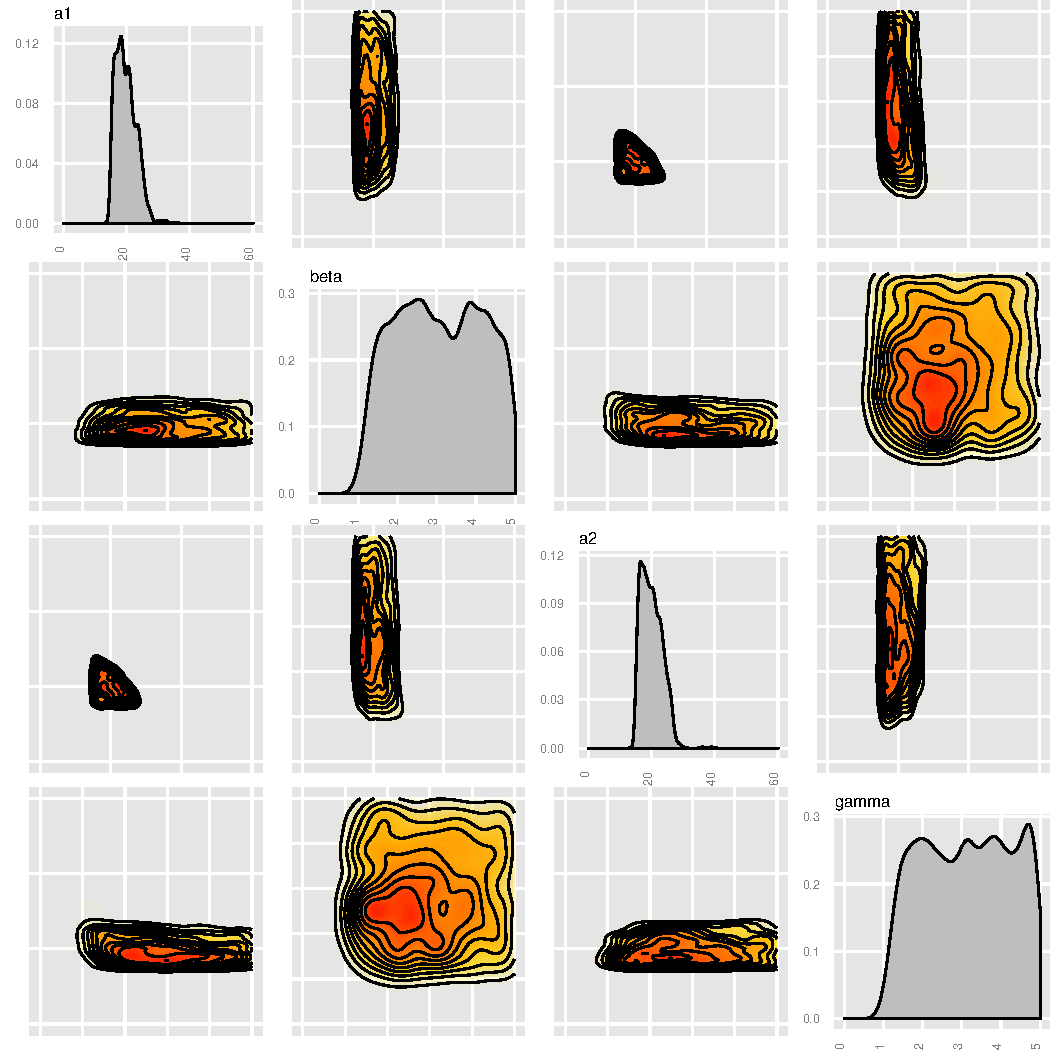
\includegraphics[scale=0.5]{chapterStabilityFinder/images/Gardner/wide_var/posterior_deter_high_mean.pdf}
%\caption{The posterior distribution of the deterministic model of the Gardner toggle switch.}
%\label{fig:Gard_post_det_high}
%\end{figure}
%
%\begin{figure}[p]
%\centering
%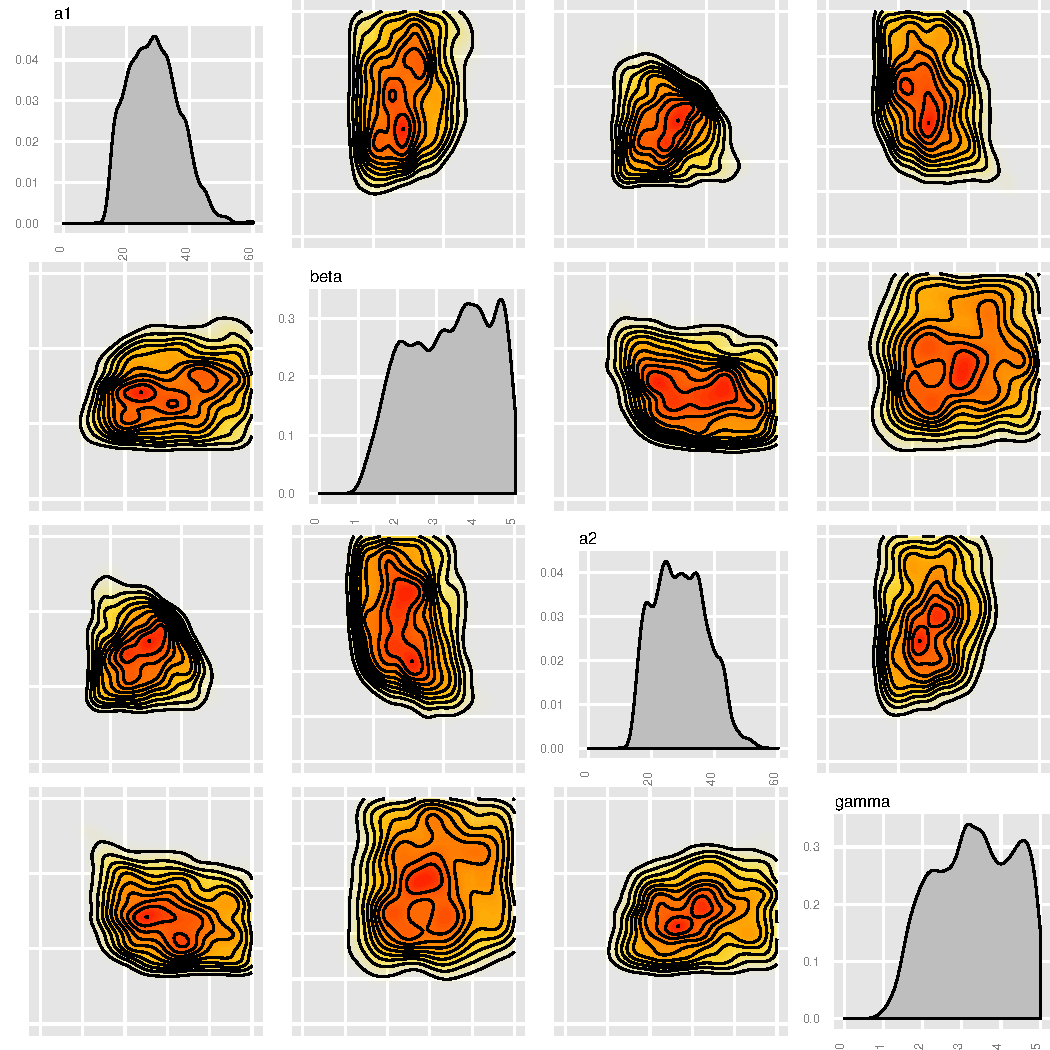
\includegraphics[scale=0.5]{chapterStabilityFinder/images/Gardner/wide_var/posterior_stch_high_mean.pdf}
%\caption{The posterior distribution of the stochastic model of the Gardner toggle switch.}
%\label{fig:Gard_post_stch}
%\end{figure}
\clearpage
As can be seen in the above results, stochasticity has a big effect on the posterior. Firstly, a greater parameter range can produce a bistable behaviour when stochastic effects are taken into account. The condition set by T.~S Gardner~\autocite{Gardner:2000vha} for the values of $a_1$ and $a_2$ to be balanced holds in both the deterministic and stochastic cases but in the stochastic case this is met by a wider range of values. The second conditions of $\beta$, $\gamma$ \textgreater 1 also needs to be met in the stochastic case. The posterior of the deterministic model shown in Figure~\ref{fig:Gard_summary}B, parameters $a_1$ and $a_2$ also have an upper limit of values they can take and still create a bistable switch. In order to test this result, we find the roots of the system for large values of  $a_1$ and $a_2$ in order to see if three roots are still found, two stable and one unstable. The results as shown in Figure indicate that the system is still bistable for increasing values of $a_1$ and $a_2$. This suggests that the upper limit found with StabilityFinder is an artefact of the variance limit imposed on the system. In order to find the steady states we impose an accepted distance from a given total variance for each model. When the two clusters of steady state values are too far removed, this increases total variance of the system and would consequently be rejected in StabilityFinder.

\begin{figure}[h]
\centering
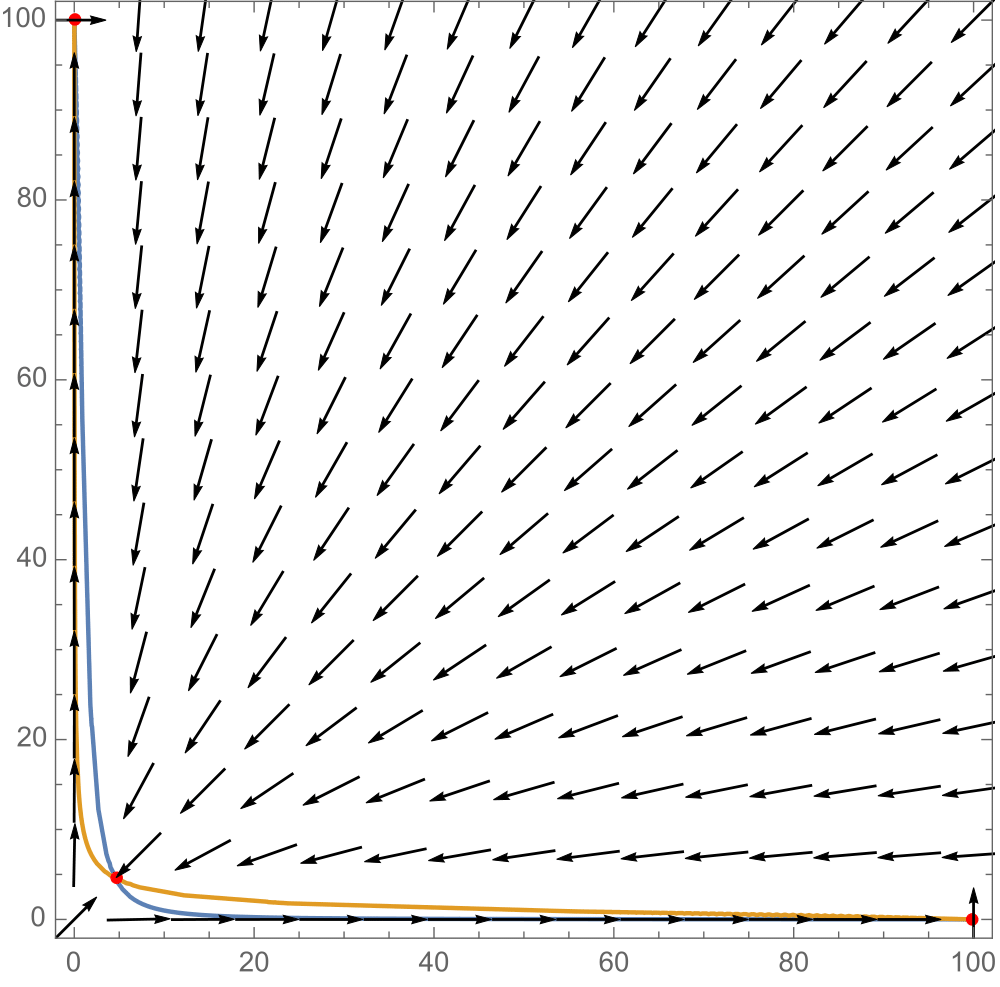
\includegraphics[scale=0.2]{chapterStabilityFinder/images/Gardner/gardner_solve_roots_a1a2_big.png}
\caption[Solving the Gardner toggle switch.]{Solving the Gardner toggle switch. The parameters values used are:  $a_1$, $a_2$ = 100 and $\beta$, $\gamma$ = 2. The system has three roots, of which one was found to be unstable and the other two stable. This result disagrees with that found in StabilityFinder, that $a_1$ and $a_2$ have an upper limit of 30.}
\label{fig:Gard_robst}
\end{figure}

 When stochasticity is taken into account, robustness increases significantly as seen in Figure~\ref{fig:Gard_robst}. This indicates that stochasticity increases the ability of the model to withstand fluctuations in parameter values and still produce the desired bistability. A deterministic model cannot predict this increased robustness.
 
\begin{figure}[h]
\centering
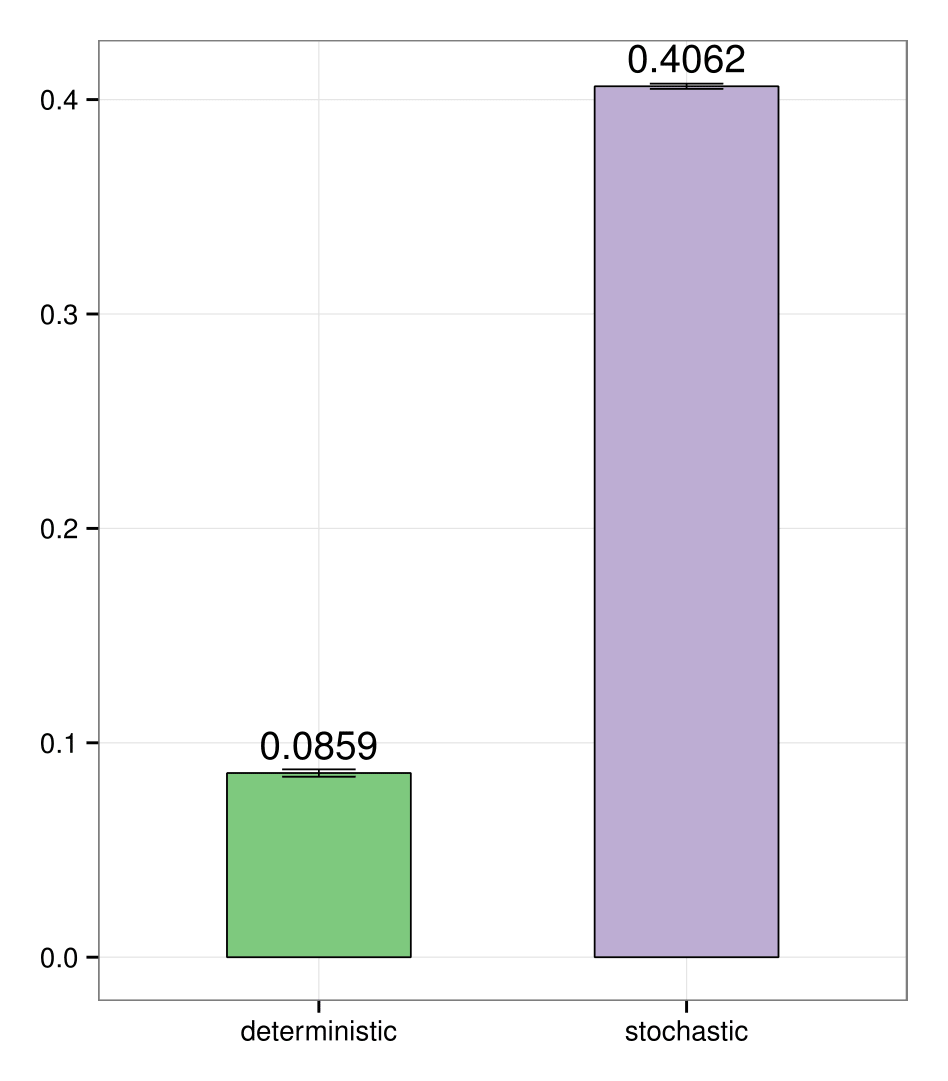
\includegraphics[scale=0.2]{chapterStabilityFinder/images/Gardner/robustness_comparison_det_stch.png}
\caption{Comparing the robustness of the deterministic and stochastic Gardner switch models}
\label{fig:Gard_robst}
\end{figure}



In order to check if this increase in robustness is caused by the different clustering methods used in the stochastic and deterministic cases, we tested the deterministic case by running the exact same model but using the clustering algorithm used in the stochastic case. Then we compared the robustness using the method outlined above. These results are shown in Figure~\ref{fig:Gard_det_stoch_kmeans}

\begin{figure}[h]
\centering
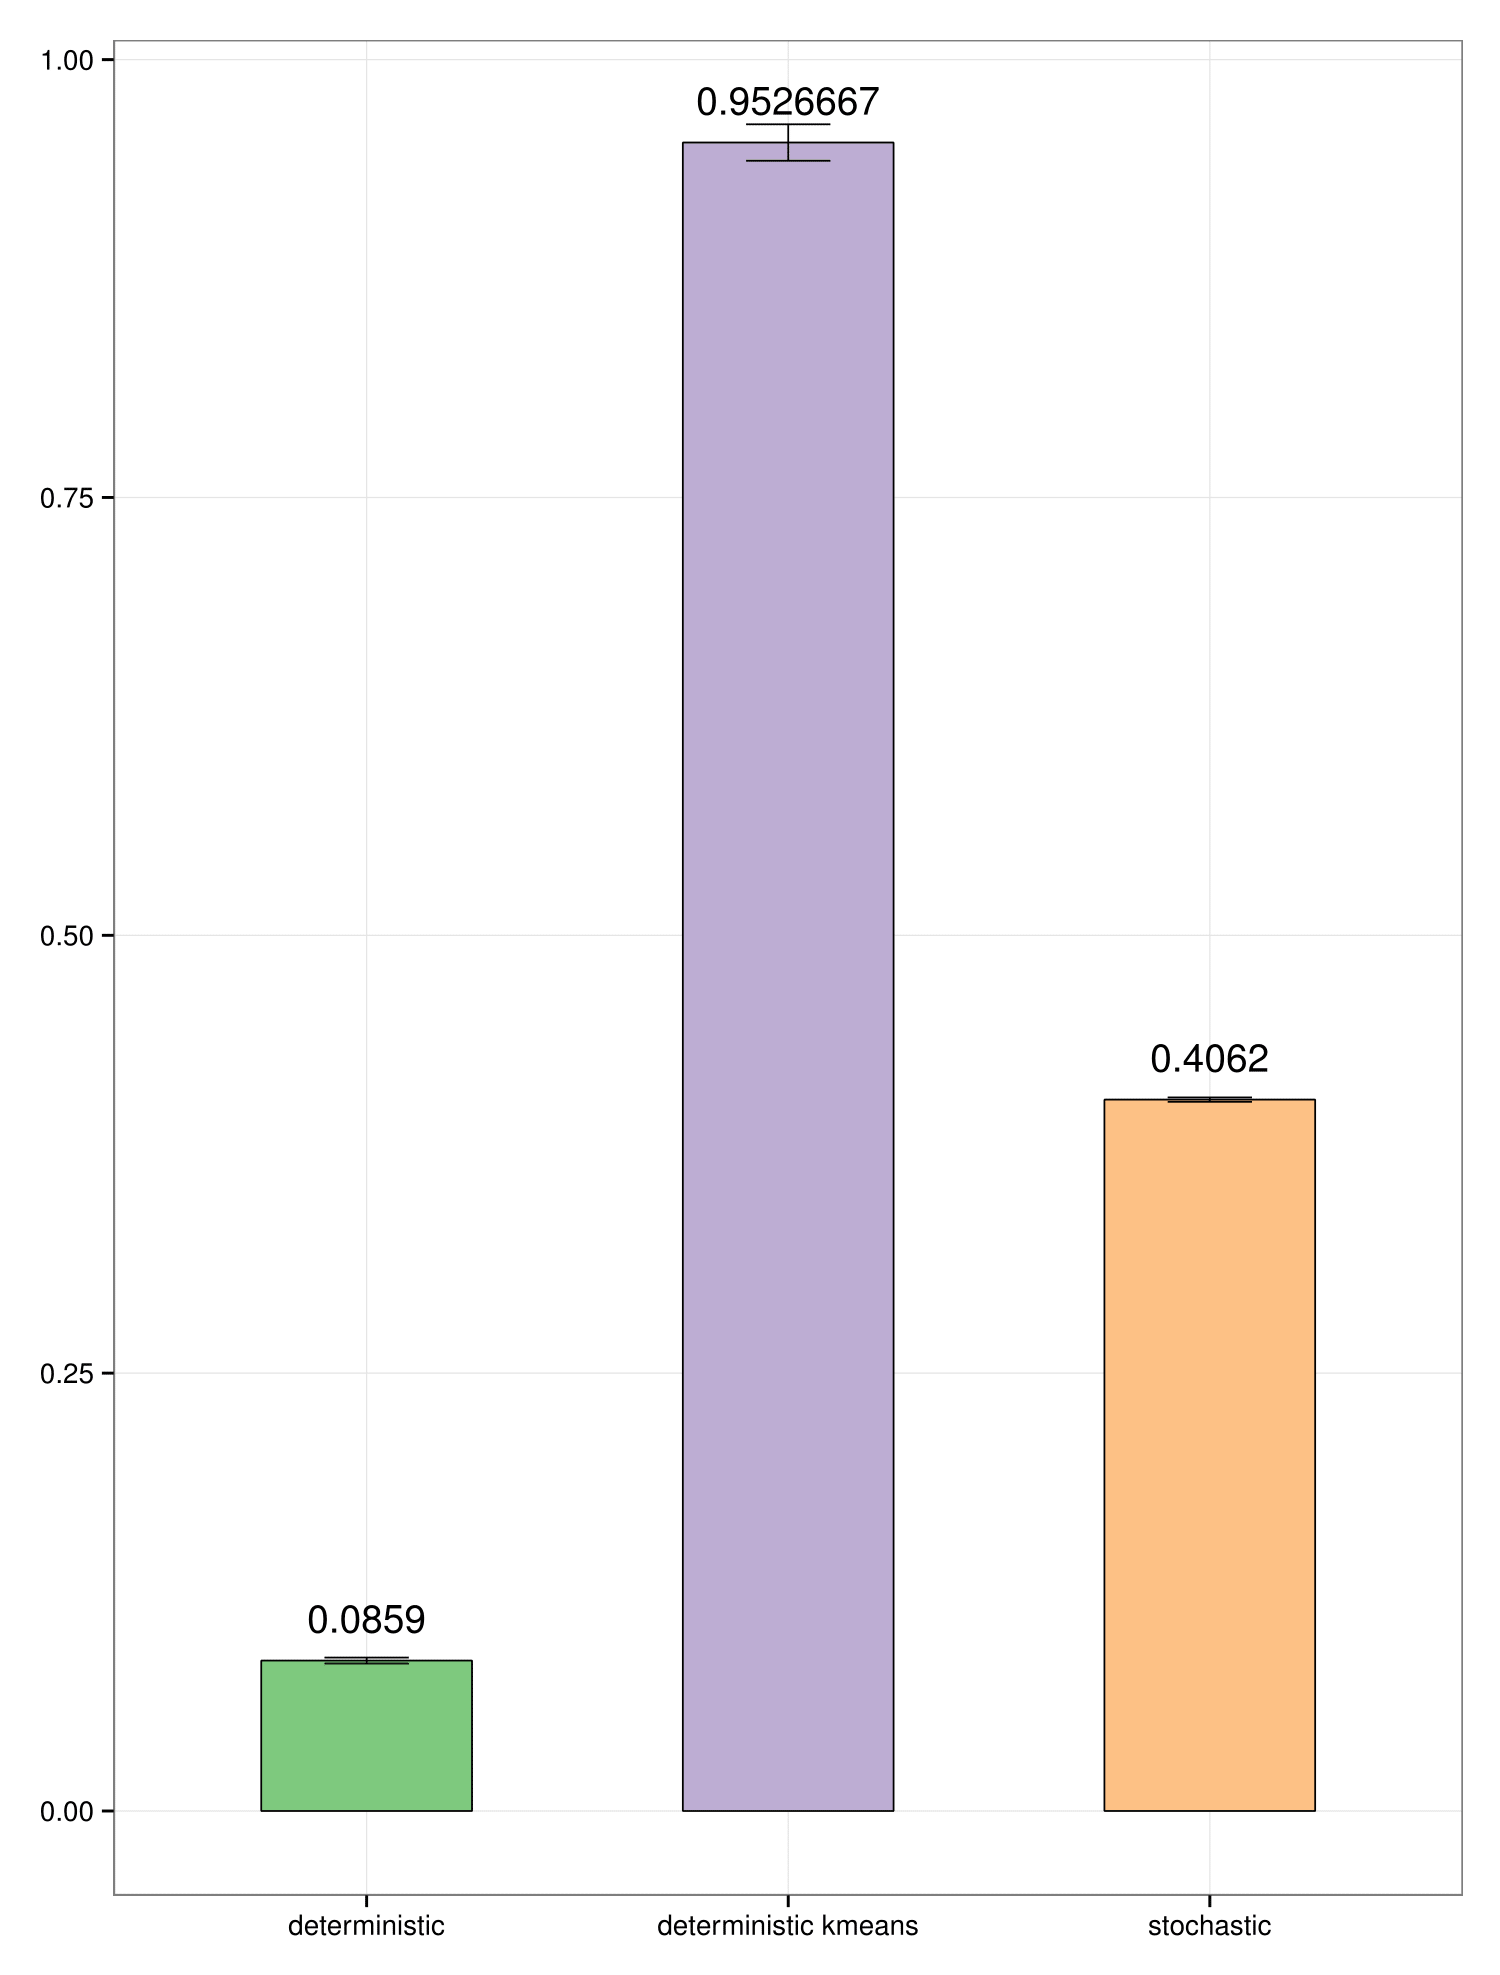
\includegraphics[scale=0.15]{chapterStabilityFinder/images/Gardner/robustness_comparison_gard_stoch_determ_kmeans.png}
\caption{The effect of the clustering methods on robustness measurements}
\label{fig:Gard_det_stoch_kmeans}
\end{figure}

This indicates that the clustering methods used have a big effect on the robustness measured. The increase in robustness seen in Figure~\ref{fig:Gard_robst} could be a bias of the clustering algorithms.
\clearpage

%\section{Lu toggle switch models}
In their study, \cite{Lu:2013br} explored the effect of white Gaussian and shot noise on the multi-state switches. They found that the classical toggle switch, with the repressing transcription factors has two steady states and the toggle switch with added double positive auto-regulation has three steady states. By extending the analysis on these models by using StabilityFinder we can determine the design principles that make a tristable versus a bistable switch. This is another example of a use for StabilityFinder.
The system used in their study is defined by two dynamical systems:

\begin{align}
\dot{x} &= f_{x}(x,y) =g_{x}\, H^{S}_{xy}(y)\, H^{S}_{xx}\,(x)-k_{x}x \label{eq:lu_both_1} \\
\dot{y} &= f_{y}(x,y) =g_{y}\,H^{S}_{yx}(x)\,H^{S}_{yy}\,(y)-k_{y}y \label{eq:lu_both_2}
\end{align}
\begin{align}
H^{S}_{xx} &= H^{-}_{x}(x)+\lambda_{x}H^{+}_{x}(x)\label{eq:lu_hsxx}\\
H^{-}_{x}(x) &= 1 \big/\left[1+(x/a_{x})^{n_{x}}\right]\label{eq:lu_hpx}\\
H^{+}_{x}(x) &= 1-H^{-}_{x}(x)\label{eq:lu_hmx}
\end{align}
%\begin{align*}%
%	\left\{S^3_\text{this} \frac{1}{2}\right.
%\end{align*}

The three switches are illustrated in Figure~\ref{fig:lu_sketch} below. 


\begin{figure}[htbp]
\centering
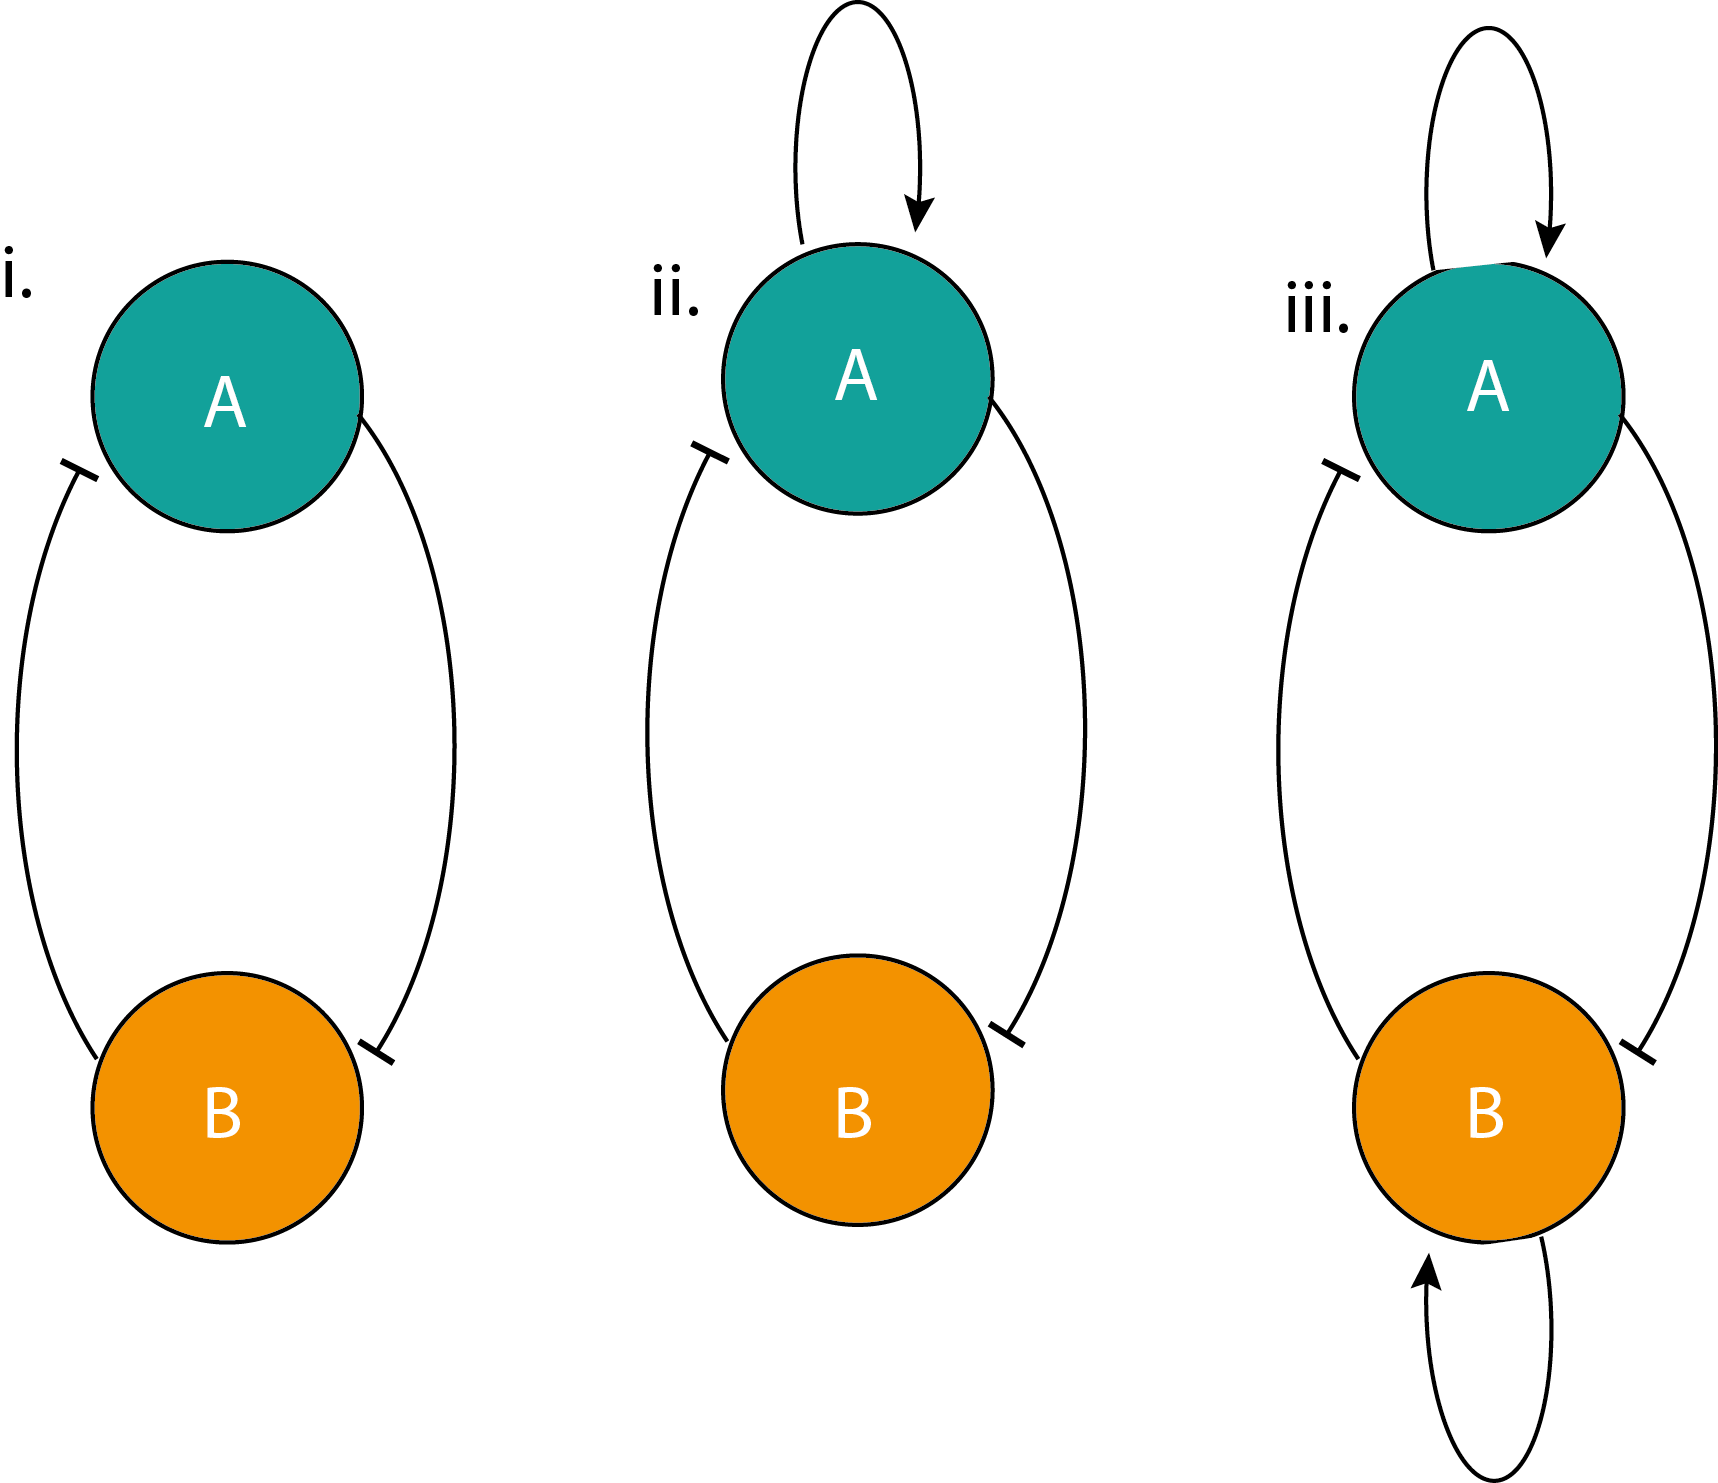
\includegraphics[scale=0.5]{chapterStabilityFinder/Lu_switches/images/lu_three_switches_sketch.png}
\caption[Lu switches]{The three Lu switches studied. (i) is the classical model with no self activation, (ii) has a single positive autoregulation and (iii) has double positive autoregulation. }
\label{fig:lu_sketch}
\end{figure}


\clearpage

\subsection{Classical model}
For the classical model, in which no self-activation is present, the system reduces to the following equations:

\begin{align}
\dot{x}=f_{x}(x,y) &= g_{x}H^{S}_{xy}(y)-k_{x}x,\label{eq:lu_cl_1}\\
\dot{y}=f_{y}(x,y) &= g_{y}H^{S}_{yx}(x)-k_{y}y\label{eq:lu_cl_2}
\end{align}
For the parameter values used in the Lu study, as shown in Table ~\ref{tab:lu_cl_bi}, the system exhibits three steady states (Figure ~\ref{fig:lu_bis_class}), of which two are stable and one is unstable. 

\begin{table}[htbp]
\centering
\caption{Lu classical model parameter values}
\label{tab:lu_cl_bi}
\begin{tabular}{cccccccccc}
gx    & gy    & kx    & ky    & nxy & nyx & xxy     & xyx     & Ixy   & Iyx \\
40&40     &0.1   & 0.1   &  3  &  3  &  200    &  200    & 0.1    &   0.1
\end{tabular}
\end{table}

\begin{figure}[htbp]
\centering
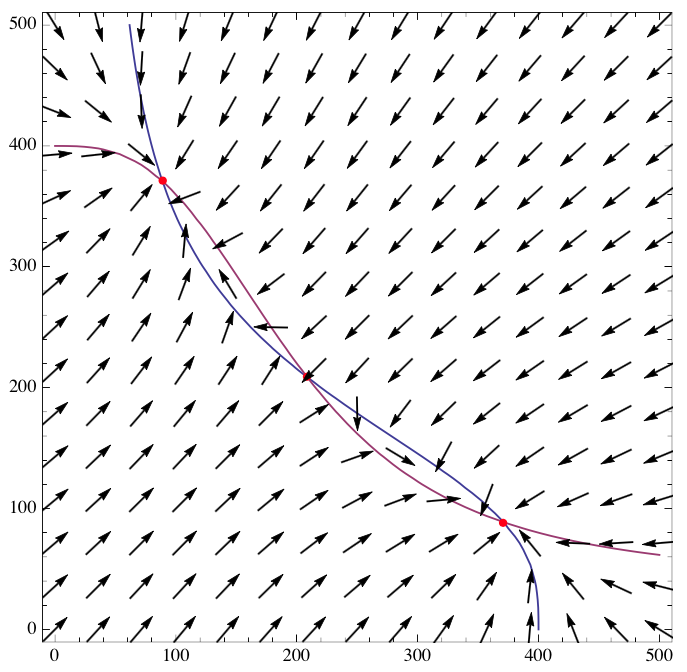
\includegraphics[scale=0.4]{chapterStabilityFinder/Lu_switches/images/mae/classical_bistable.png}
\caption[Phase portrait of the Lu classical model with no self activation]{Phase portrait of the Lu classical model with no self activation. There are two stable steady states and one unstable steady state.}
\label{fig:lu_bis_class}
\end{figure}


\clearpage

Using StabilityFinder with priors centred around the parameter values used in the original paper (Table ~\ref{tab:lu}), we can find the robustness of this bistable behaviour, as well as identify the most important parameters for bistability. 
\begin{table}[h]
\centering
\caption{Lu classical model priors}
\label{tab:lu}
\begin{tabular}{cccccccccc}
gx    & gy    & kx    & ky    & nxy & nyx & xxy     & xyx     & Ixy   & Iyx \\
35-45 & 35-45 & 0-0.2 & 0-0.2 & 2-4 & 2-4 & 150-250 & 150-250 & 0-0.2 &   0-0.2 
\end{tabular}
\end{table}

The posterior distribution of this model is shown in Figure~\ref{fig:lu_bistable}. As can be seen from the posterior, the most restrained parameters are kx and ky, the parameters responsible for the degradation of the species involved. This indicates that the rate of degradation of the species is critical for the desired dynamic to occur. 

\begin{figure}[htbp]
\centering
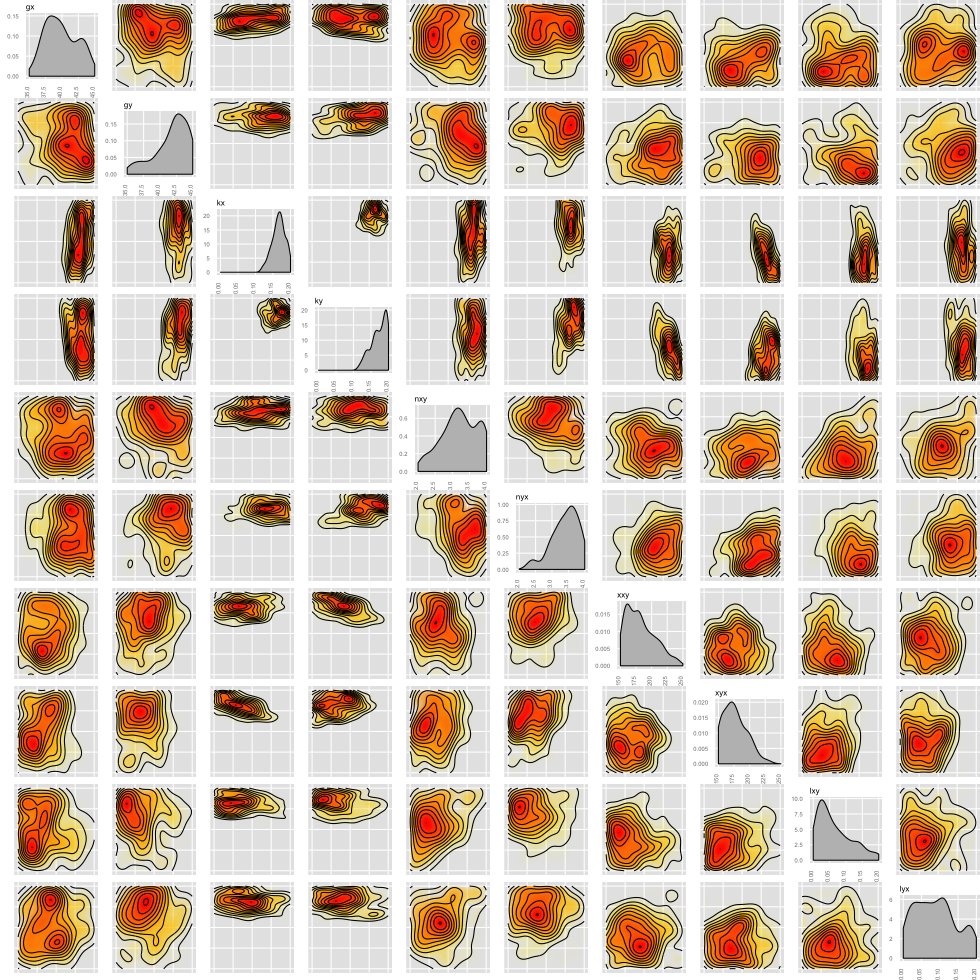
\includegraphics[scale=0.25]{chapterStabilityFinder/Lu_switches/images/classic/posterior_lu_cl.png}
\caption[The posterior distribution of the Lu classical model with no self activation]{The posterior distribution of the Lu classical model with no self activation. kx and ky are the most constrained parameters.}
\label{fig:lu_bistable}
\end{figure}

\begin{figure}[htbp]
\centering
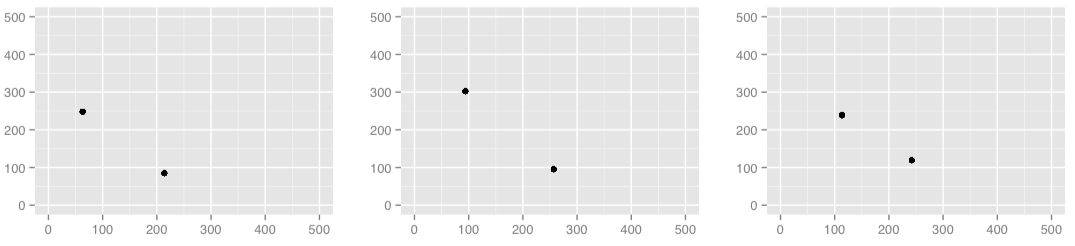
\includegraphics[scale=0.2]{chapterStabilityFinder/Lu_switches/images/classic/phase_plot.png}
\caption{A sample of the phase plots produced from the final population of the Lu classical model.}
\label{fig:lu_phase}
\end{figure}
\clearpage

\subsection{Single positive autoregulation}

If single self-activation is included, then the system is that presented in equations \ref{eq:lu_both_1} - \ref{eq:lu_hmx}. Using the priors used in Table~\ref{tab:lu_sp_pr}, the posterior distribution of for this bistable switch is that shown in Figure~\ref{fig:lu_sp_pos}. 

\begin{table}[htbp]
\centering
\caption{Lu model with single self-activation priors}
\label{tab:lu_sp_pr}
\begin{tabular}{cc}
parameter & range \\
gx & 1-2 \\
gy & 20-25 \\
kx & 50-55 \\
ky & 48-52 \\
nxy & 30-35 \\
nyx & 0.1-0.2 \\
xxy & 2-3 \\
xyx & 0.4-0.6 \\
lxy & 0.02-0.04 \\
lyx & 0.02-0.04 \\
nXX & 25-30  \\
nYY & 0.01-0.02 \\
xXX & 0.4-0.5 \\
xYY & 1-3 \\
lXX & 65-72 \\
lYY & 0.02-0.04
\end{tabular}
\end{table}


\begin{figure}[t]
\centering
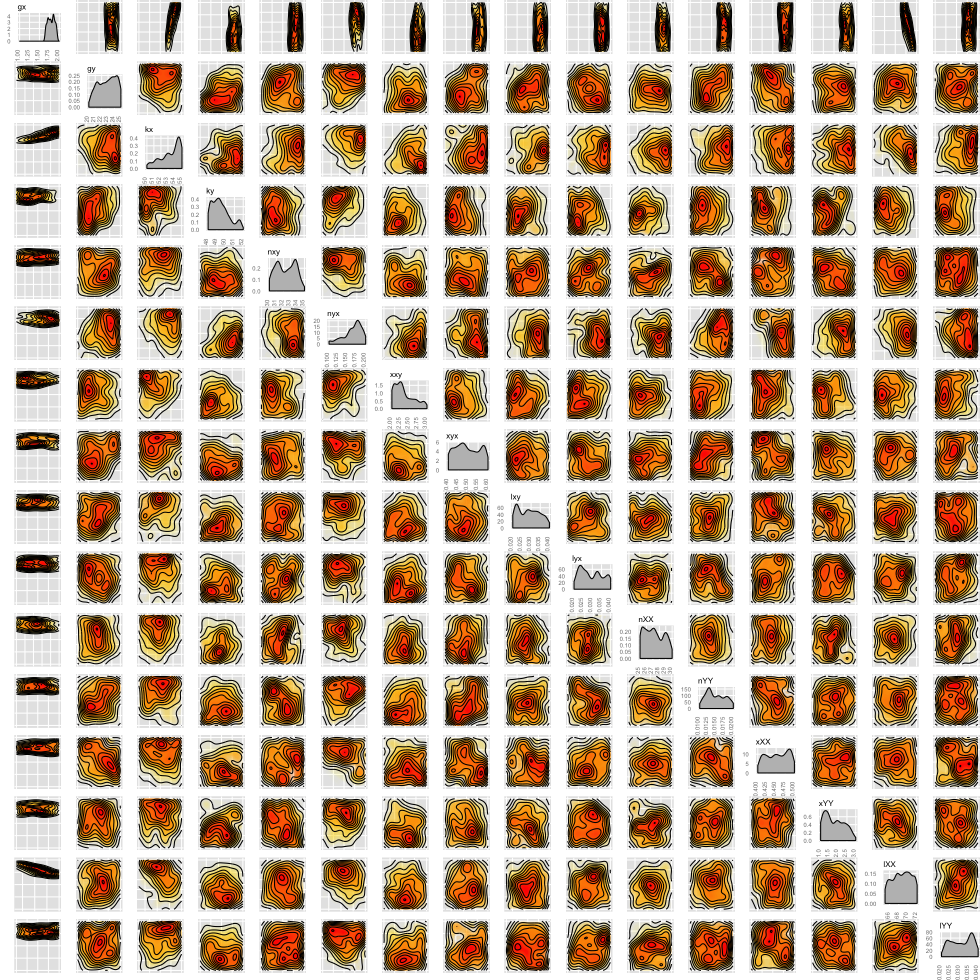
\includegraphics[scale=0.35]{chapterStabilityFinder/Lu_switches/images/single_pos/posterior_lu_sp_bis.png}
\caption[The posterior distribution of the Lu model with asymmetric self activation]{The posterior distribution of the Lu model with asymmetric self activation}
\label{fig:lu_sp_pos}
\end{figure}

\begin{figure}[t]
\centering
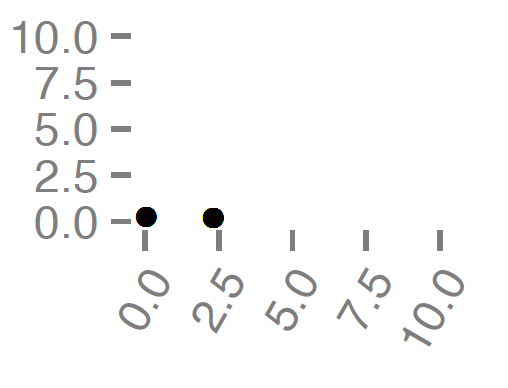
\includegraphics[scale=0.2]{chapterStabilityFinder/Lu_switches/images/single_pos/phase_plot.png}
\caption{Phase plot of asymmetric Lu toggle switch}
\label{fig:lu_sp_phase}
\end{figure}
\clearpage

\subsection{Double positive autoregulation}
If self-activation is included, then the system is that presented in equations \ref{eq:lu_both_1} - \ref{eq:lu_hmx}. When values that are presented in Table~\ref{tab:lu_dp_tri} are assigned to the parameters for the self-activating model, the system exhibits three stable and two unstable steady states as seen in Figure~\ref{fig:lu_tri_phse}. 

\begin{table}[h]
\centering
\caption{Lu model with self-activation parameter values}
\label{tab:lu_dp_tri}
\begin{tabular}{cccccccccc}
gx    & gy    & kx    & ky    & nxy & nyx & xxy     & xyx     & Ixy   & Iyx \\
4&4     &0.1   & 0.1   &  1  &  1  &  200    &  200    & 0.1    &   0.1
\end{tabular}
\end{table}

\begin{figure}[h]
\centering
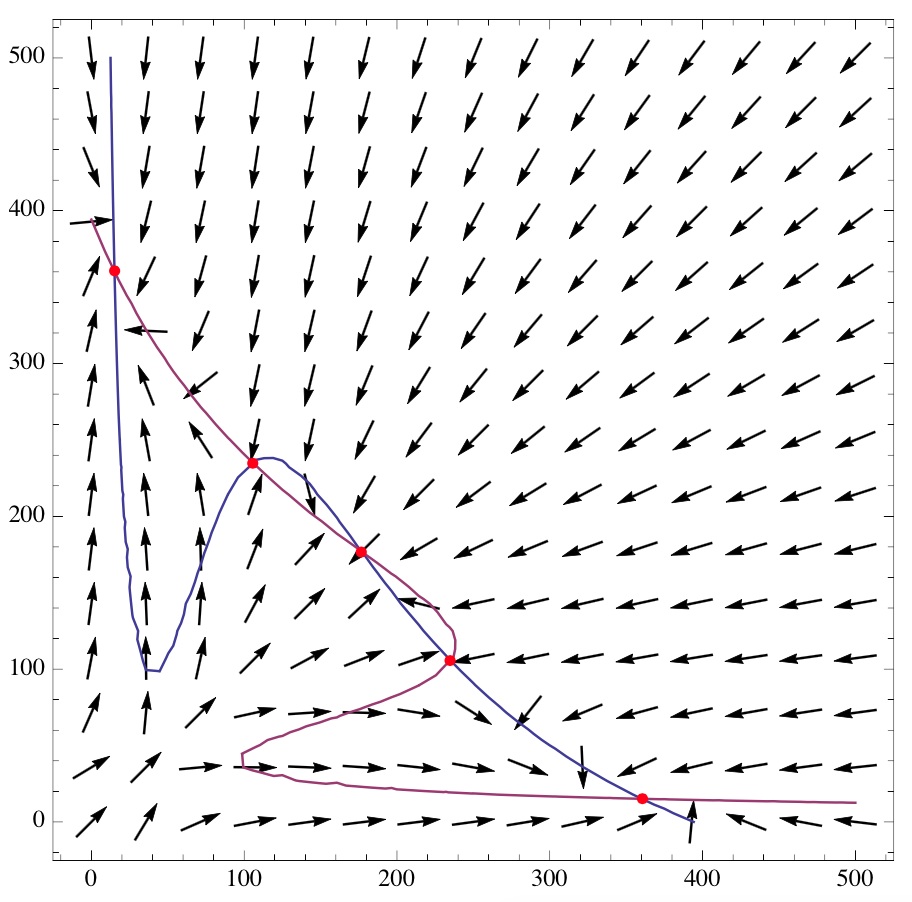
\includegraphics[scale=0.3]{chapterStabilityFinder/Lu_switches/images/mae/tristable_db.png}
\caption[Phase portrait of the Lu model including double self-activation]{Phase portrait of the Lu model including double self-activation. The model had three stable steady states and two unstable steady states.}
\label{fig:lu_tri_phse}
\end{figure}
\clearpage
Using StabilityFinder and wide priors around the original values, shown in Table~\ref{tab:lu_dp_pr}, we can explore the robustness of this behaviour, in a similar way as done for the classical model. 

\begin{table}[htbp]
\centering
\caption{Lu model with double self-activation priors}
\label{tab:lu_dp_pr}
\begin{tabular}{cc}
parameter & range \\
gx & 1-100 \\
gy & 1-100 \\
kx & 0-1 \\
ky & 0-1 \\
nxy & 0-10 \\
nyx & 0-10 \\
xxy & 100-1000 \\
xyx & 100-1000 \\
lxy & 0-1 \\
lyx & 0-0.2 \\
nXX & 0-10  \\
nYY & 0-10 \\
xXX & 50-500 \\
xYY & 50-500 \\
lXX & 1-20 \\
lYY & 1-20
\end{tabular}
\end{table}

The posterior is shown in Figure~\ref{fig:lu_tristable}. 
\begin{figure}[h]
\centering
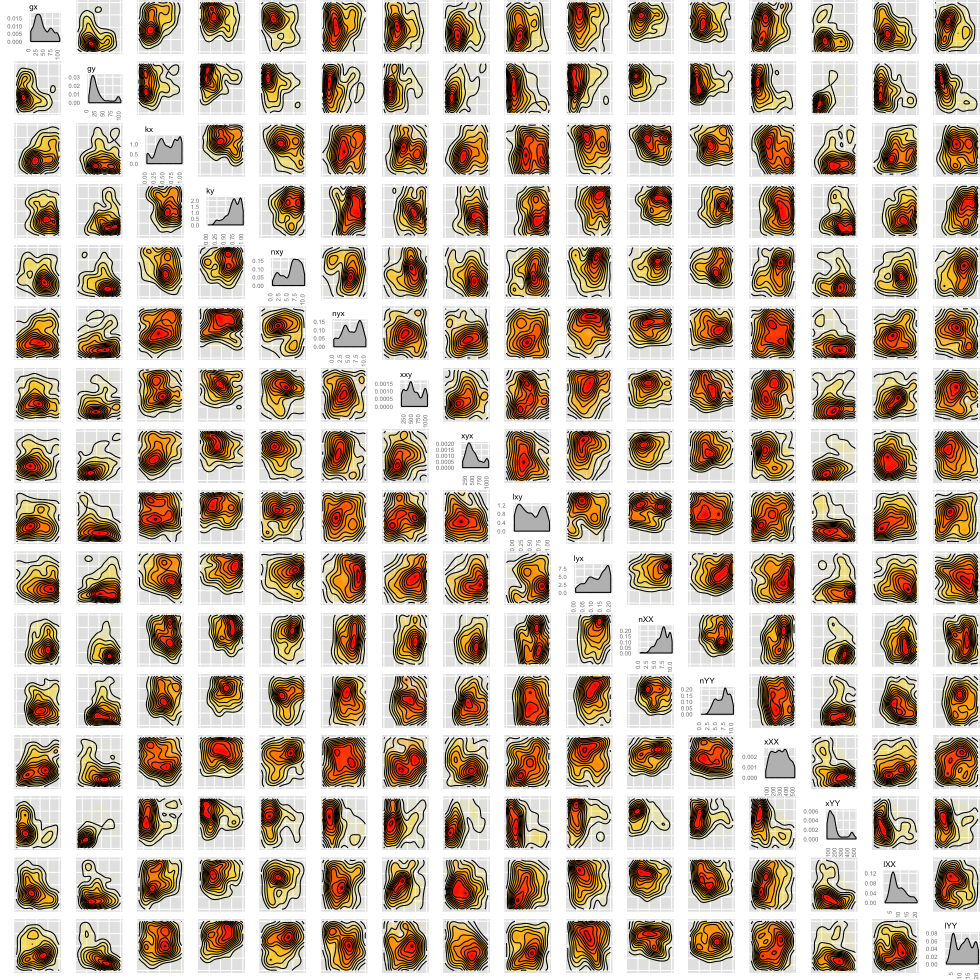
\includegraphics[scale=0.4]{chapterStabilityFinder/Lu_switches/images/double_pos/posterior_tri_wide_params.png}
\caption[The posterior distribution of the Lu model with double self activation]{The posterior distribution of the Lu model with double self activation.}
\label{fig:lu_tristable}
\end{figure}


\begin{figure}[h]
\centering
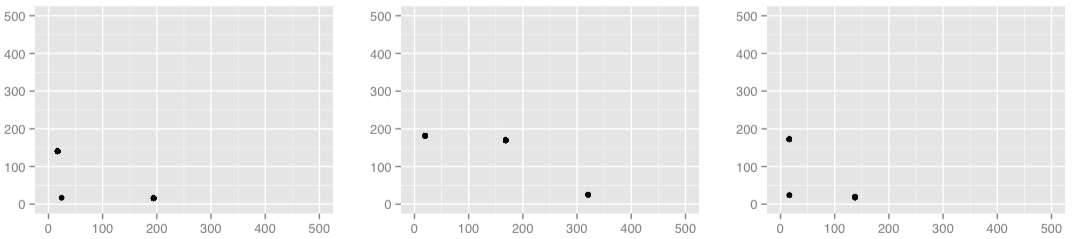
\includegraphics[scale=0.3]{chapterStabilityFinder/Lu_switches/images/double_pos/phase_plots.png}
\caption{A sample of the phase plots produced from the final population of the Lu tristable model.}
\label{fig:lu_tri_phase_pl}
\end{figure}
\clearpage
%%%%
\subsection{Extracting the design principles of a tristable switch}
Next, we went on to study the design principles that make a switch tristable vs bistable. In order to do that, first we use StabilityFinder to find the parameter space that gives rise to a bistable switch, given the same model and priors used above to find a tristable switch, as shown in Figure~\ref{fig:lu_bi_tri_cartoon}.

\begin{figure}[h]
\centering
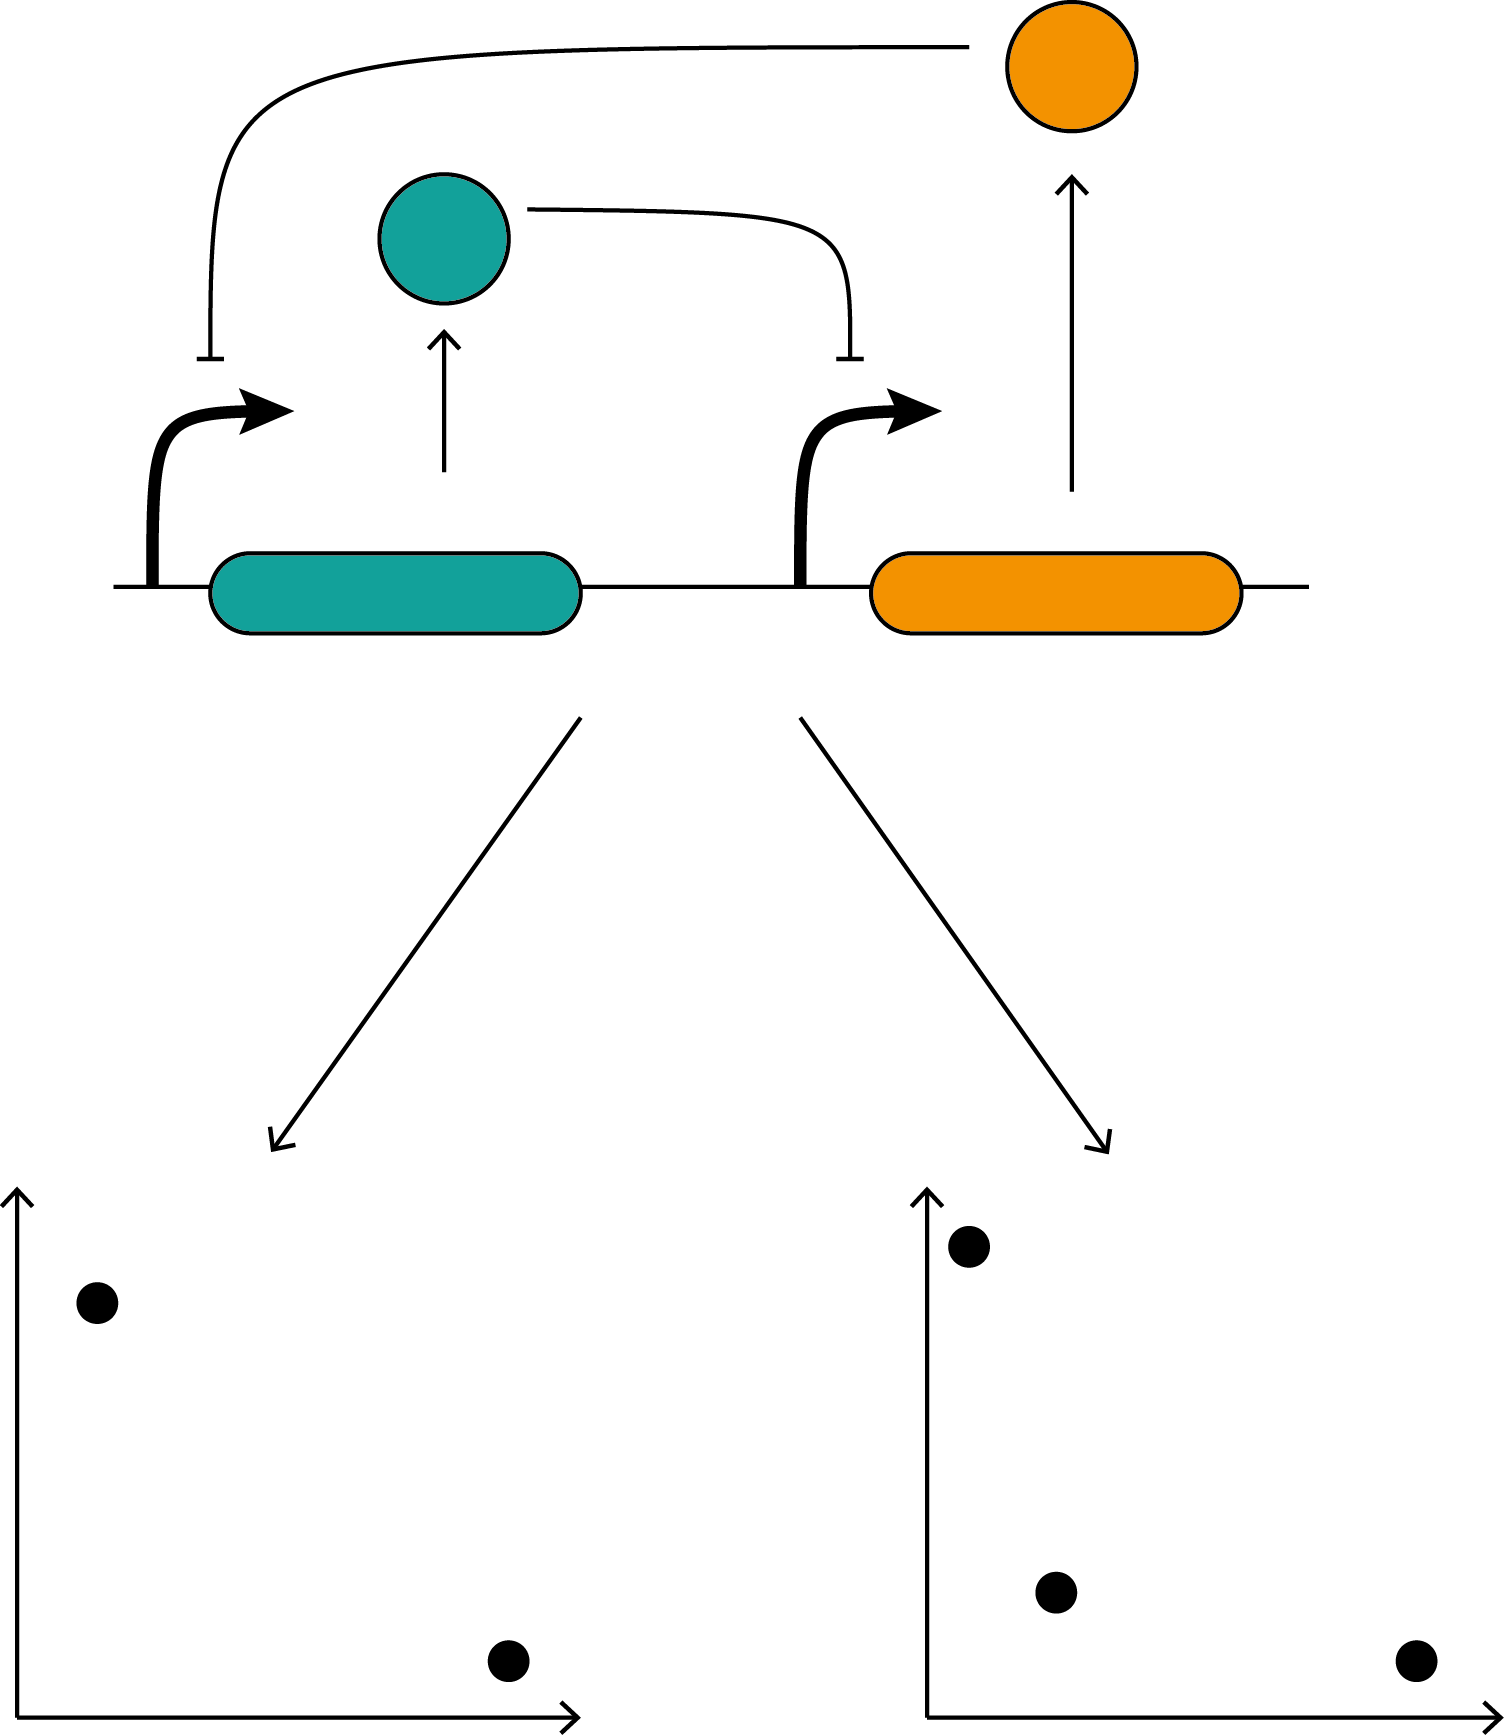
\includegraphics[scale=0.5]{chapterStabilityFinder/Lu_switches/images/double_pos/lu_bi_tri_cartoon.png}
\caption{Finding the parameter spaces that make the Lu double positive model bistable and tristable. }
\label{fig:lu_bi_tri_cartoon}
\end{figure}

By plotting the resulting posterior with that of the tristable switch shown in Figure~\ref{fig:lu_tristable} we can examine any separation of values between a bistable and a tristable switch, as shown in Figure~\ref{fig:pos_comp_lu}.

\begin{figure}[h]
\centering
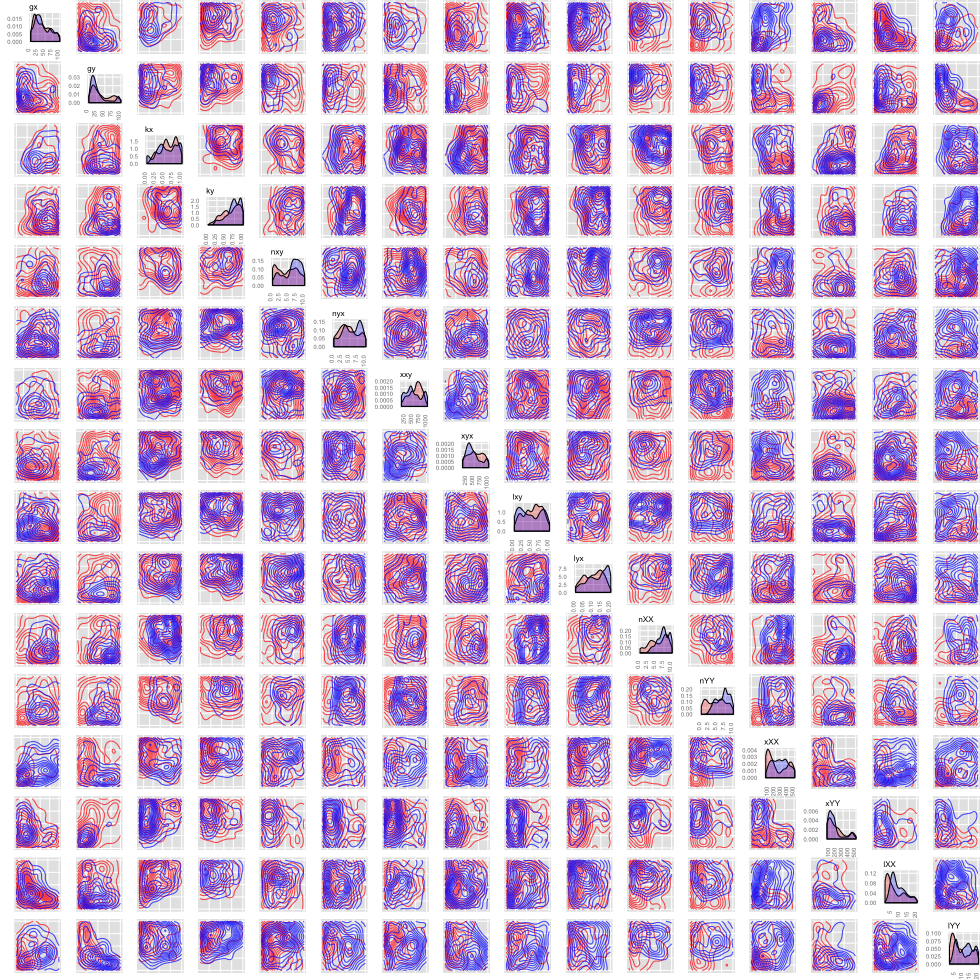
\includegraphics[scale=0.4]{chapterStabilityFinder/Lu_switches/images/double_pos/posterior_comparison_bi_tri.png}
\caption{Comparing the posteriors of the tristable Vs bistable Lu switch.}
\label{fig:pos_comp_lu}
\end{figure}
\clearpage

In order to separate the values in a more meaningful way, we implement an algorithm as outlined in Appendix. By taking samples from the posterior of a bistable switch, we keep track of the values for each parameter that are also found in the posterior of the tristable switch, and vice versa. The results are shown in Figure~\ref{fig:design_princip_lu} below:


\begin{figure}[h]
\centering
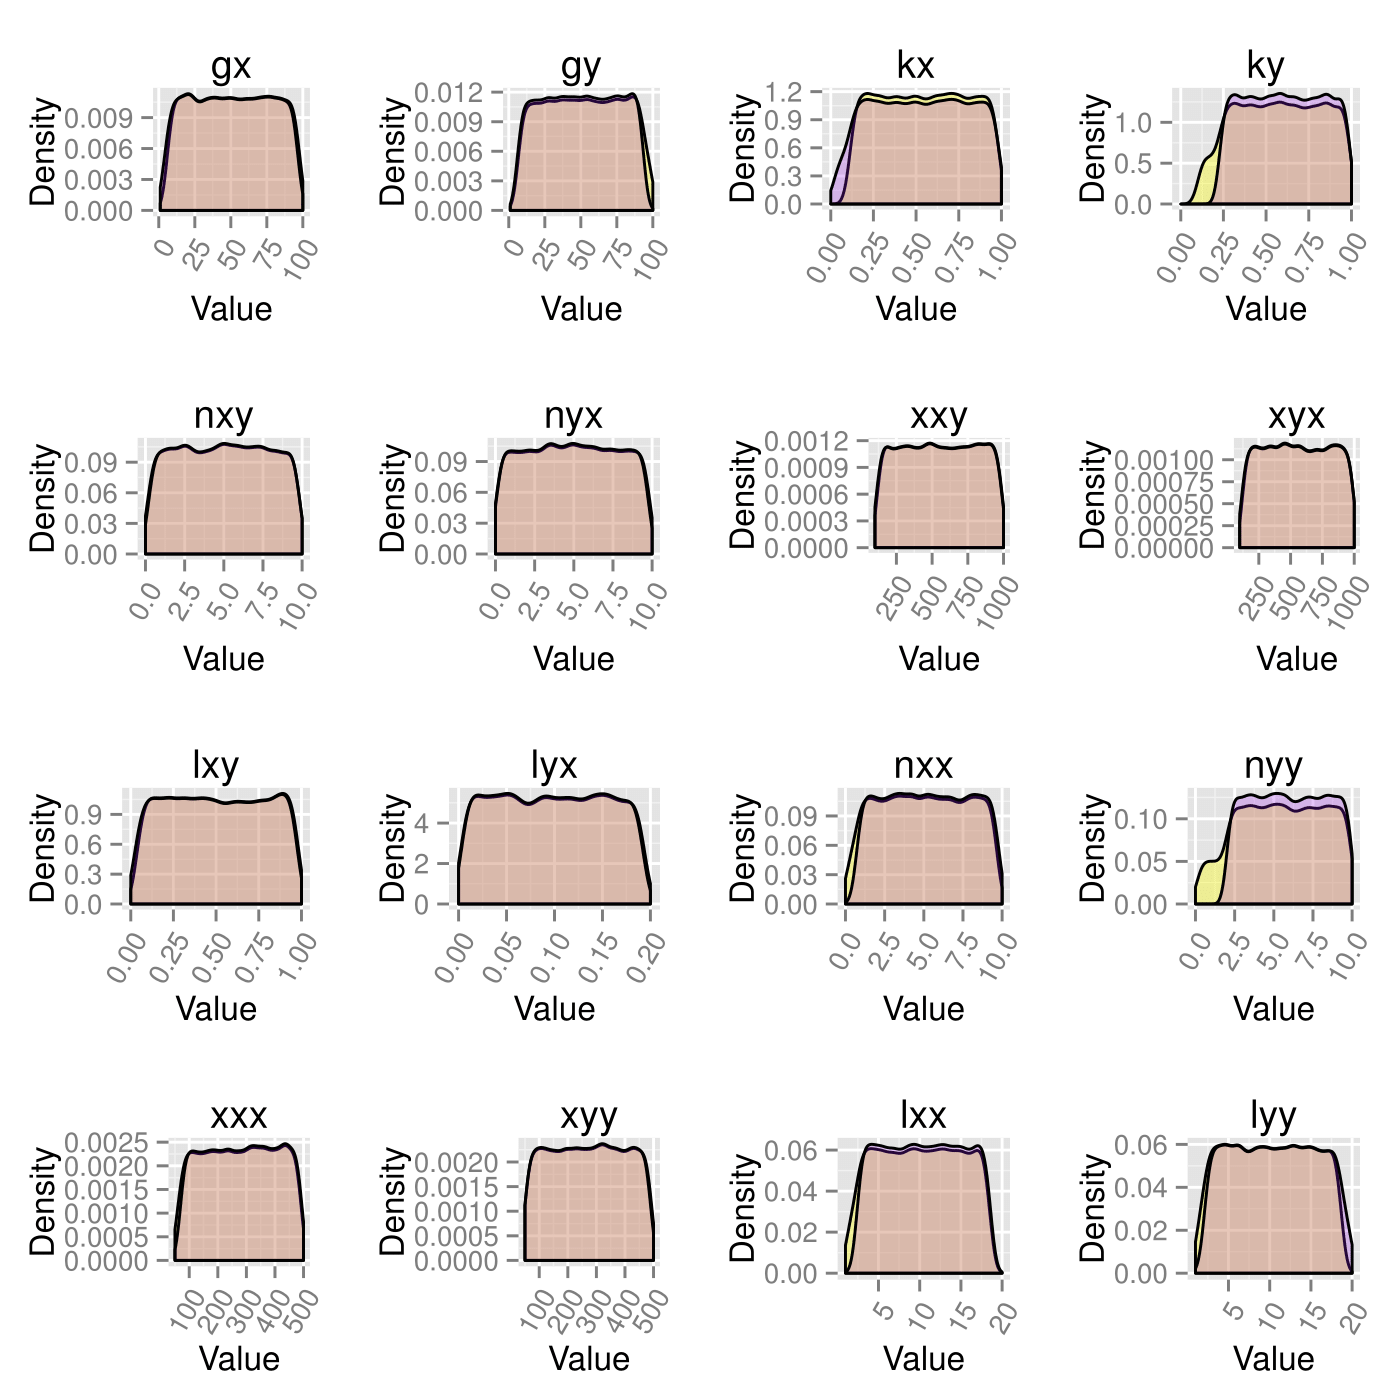
\includegraphics[scale=0.2]{chapterStabilityFinder/Lu_switches/images/double_pos/design_principles_bi_tri.png}
\caption{Design principles of the tristable Lu switch.}
\label{fig:design_princip_lu}
\end{figure}

From the results above we can conclude that there is no significant difference between a bistable and a tristable switch in parameter values. 


%\section{Mass Action switches}

When faced with a set of competing designs for a given genetic circuit, one is likely to choose the simplest possible model that can achieve the desired behaviour. However, simple systems are often the least robust. Here we define a robust device as a device that can withstand fluctuations in parameter values and still produce the desired behaviour. Feedback loops are well known key regulatory motifs \autocite{Brandman:2005ci}. Negative feedback loops are essential for homeostasis and buffering \autocite{Thomas:1995id} thus increasing robustness to extrinsic noise sources and positive feedback loops can generate multistationarity in a system \autocite{Thomas:1995id}. Incorporating this kind of additional feedback interactions can make a design more robust and reliable. Here we use StabilityFinder to compare the robustness of two switches, a simple toggle switch and a switch with added positive auto-regulation. 
In order to study this system in the most realistic way, we avoid using the quasi-steady state approximation (QSSA) that is often used in modelling the toggle switch. The QSSA assumes that the binding/unbinding processes are much faster than any other process \autocite{Loinger:2007vma} thus the bound intermediate is assumed to always be in steady state. The QSSA is often used since it reduces the dimensions of the system thus reducing computational time \autocite{Pedersen:2007ke}. The QSSA assumption is met in vitro but often does not hold in vivo. Its misuse can lead to large errors and incorrectly estimated parameters \autocite{Pedersen:2007ke}. Parameter estimation is central to this project and since StabilityChekcker is able to analyse models with numerous equations and parameters, there is no need for this assumption, which approximates a solution. Using Mass Action, the two models used are shown below:

Standard toggle switch:
$$
\begin{array}{cccc}
      \textrm{gA}\stackrel{\textrm{ge}}{\longrightarrow}\textrm{gA} + \textrm{A} \\
      \textrm{gB}\stackrel{\textrm{ge}}{\longrightarrow}\textrm{gB} + \textrm{B} \\
      \textrm{A} + \textrm{A} \stackrel{\textrm{dim}}{\longrightarrow}\textrm{A2} \\
      \textrm{A2} \stackrel{\textrm{dim r}}{\longrightarrow}\textrm{A} + \textrm{A} \\
      \textrm{B} + \textrm{B} \stackrel{\textrm{dim}}{\longrightarrow} \textrm{B2} \\
      \textrm{B2} \stackrel{\textrm{dim\_r}}{\longrightarrow}\textrm{B} + \textrm{B} \\
      \textrm{gA} + \textrm{B2} \stackrel{\textrm{rep}}{\longrightarrow}\textrm{B2gA} \\
      \textrm{B2gA} \stackrel{\textrm{rep\_r}}{\longrightarrow}\textrm{B} + \textrm{gA} \\
      \textrm{gB} + \textrm{A2} \stackrel{\textrm{rep}}{\longrightarrow}\textrm{A2gB} \\
      \textrm{A2gB} \stackrel{\textrm{rep\_r}}{\longrightarrow}\textrm{A2} + \textrm{gB} \\
      \textrm{A} \stackrel{\textrm{deg}}{\longrightarrow}\textrm{\O}\\
      \textrm{B} \stackrel{\textrm{deg}}{\longrightarrow}\textrm{\O}\\
      \textrm{S} + \textrm{A2} \stackrel{\textrm{rep\_dim}}{\longrightarrow}\textrm{SA2}\\
      \textrm{SA2} \stackrel{\textrm{rep\_dim\_r}}{\longrightarrow}\textrm{S} + \textrm{A2}\\
      \textrm{R} + \textrm{B2} \stackrel{\textrm{rep\_dim}}{\longrightarrow}\textrm{RB2}\\
      \textrm{RB2} \stackrel{\textrm{rep\_dim\_r}}{\longrightarrow}\textrm{R} + \textrm{B2}\\
      \textrm{R} \stackrel{\textrm{deg}}{\longrightarrow} \textrm{\O}\\
      \textrm{S} \stackrel{\textrm{deg}}{\longrightarrow}\textrm{\O}\\
\end{array}
$$

Double positive autoregulation:
$$
\begin{array}{cccc} 
    \textrm{A2} + \textrm{gA} \stackrel{\textrm{aut 1}}{\longrightarrow} \textrm{A2gA} \\
    \textrm{A2gA} \stackrel{\textrm{aut 2}}{\longrightarrow} \textrm{A} + \textrm{A2gA}\\
    \textrm{A2gA} \stackrel{\textrm{aut 3}}{\longrightarrow} \textrm{A2}+ \textrm{gA}  \\
    \textrm{B2} + \textrm{gB} \stackrel{\textrm{aut 1}}{\longrightarrow} \textrm{B2gB} \\
    \textrm{B2gB} \stackrel{\textrm{aut 2}}{\longrightarrow} \textrm{B} + \textrm{B2gB}\\
    \textrm{B2gB} \stackrel{\textrm{aut 3}}{\longrightarrow} \textrm{B2}+ \textrm{gB}  \\
\end{array}
$$

\subsection{Deterministic case}
\subsubsection{Symmetric switch}
Using the same priors for their shared parameters, we used StabilityFinder for both models in order to compare their robustness. The corresponding posterior distributions can be seen in Figures~\ref{fig:det_std} and ~\ref{fig:doub_pos}.

\begin{table}[p]
\centering
\caption{Mass Action switches priors}
\label{tab:simp}
\begin{tabular}{cccccccccc}
ge   & rep  & rep\_r & dim  & dim\_r & deg & deg\_dim & aut\_1 & aut\_2 & aut\_3\\
1-10 & 1-10 & 1-10    & 1-10 & 0-5    & 1-10 & 0-0.5   &1-10&5-10&1-5
\end{tabular}
\end{table}


\begin{figure}[p]
\centering
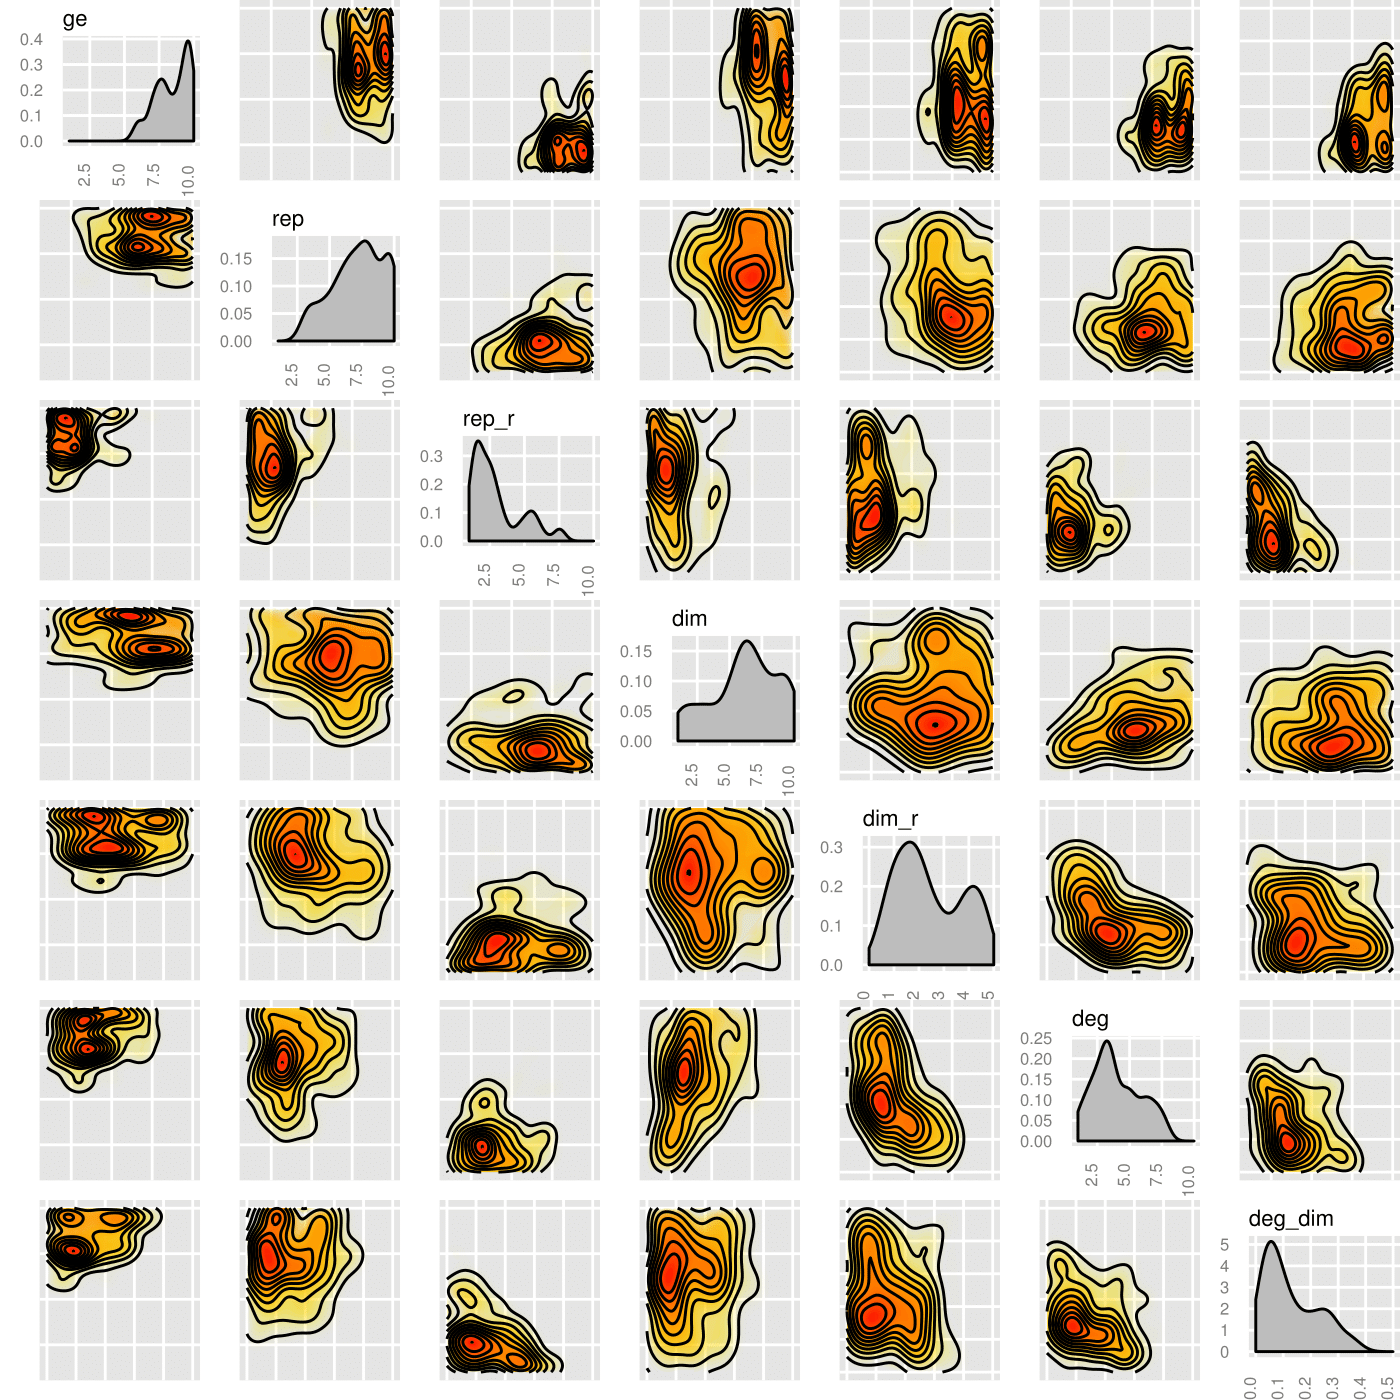
\includegraphics[scale=0.2]{chapterStabilityFinder/mass_action_switches/deterministic/posterior_ma_cl_bi.png}
\caption{The posterior distribution of the mass action simple toggle switch}
\label{fig:det_std}
\end{figure}

\begin{figure}[p]
\centering
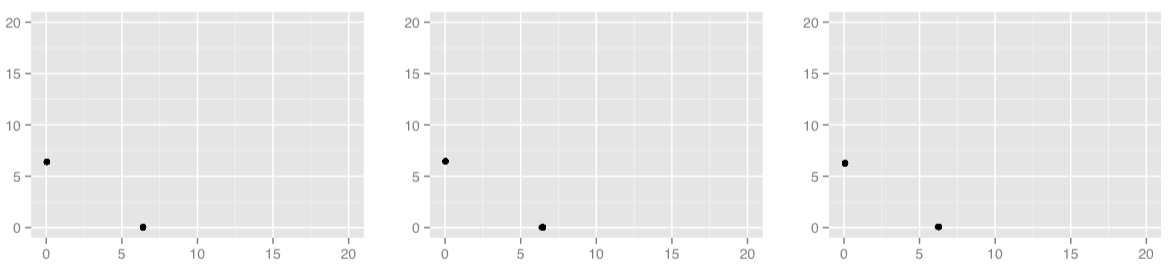
\includegraphics[scale=0.3]{chapterStabilityFinder/mass_action_switches/deterministic/ma_cl_bi_phase_plot.png}
\caption{A sample of the phase plots produced from the final population of the mass action simple toggle switch.}
\label{fig:det_std_phase}
\end{figure}

\begin{figure}[p]
\centering
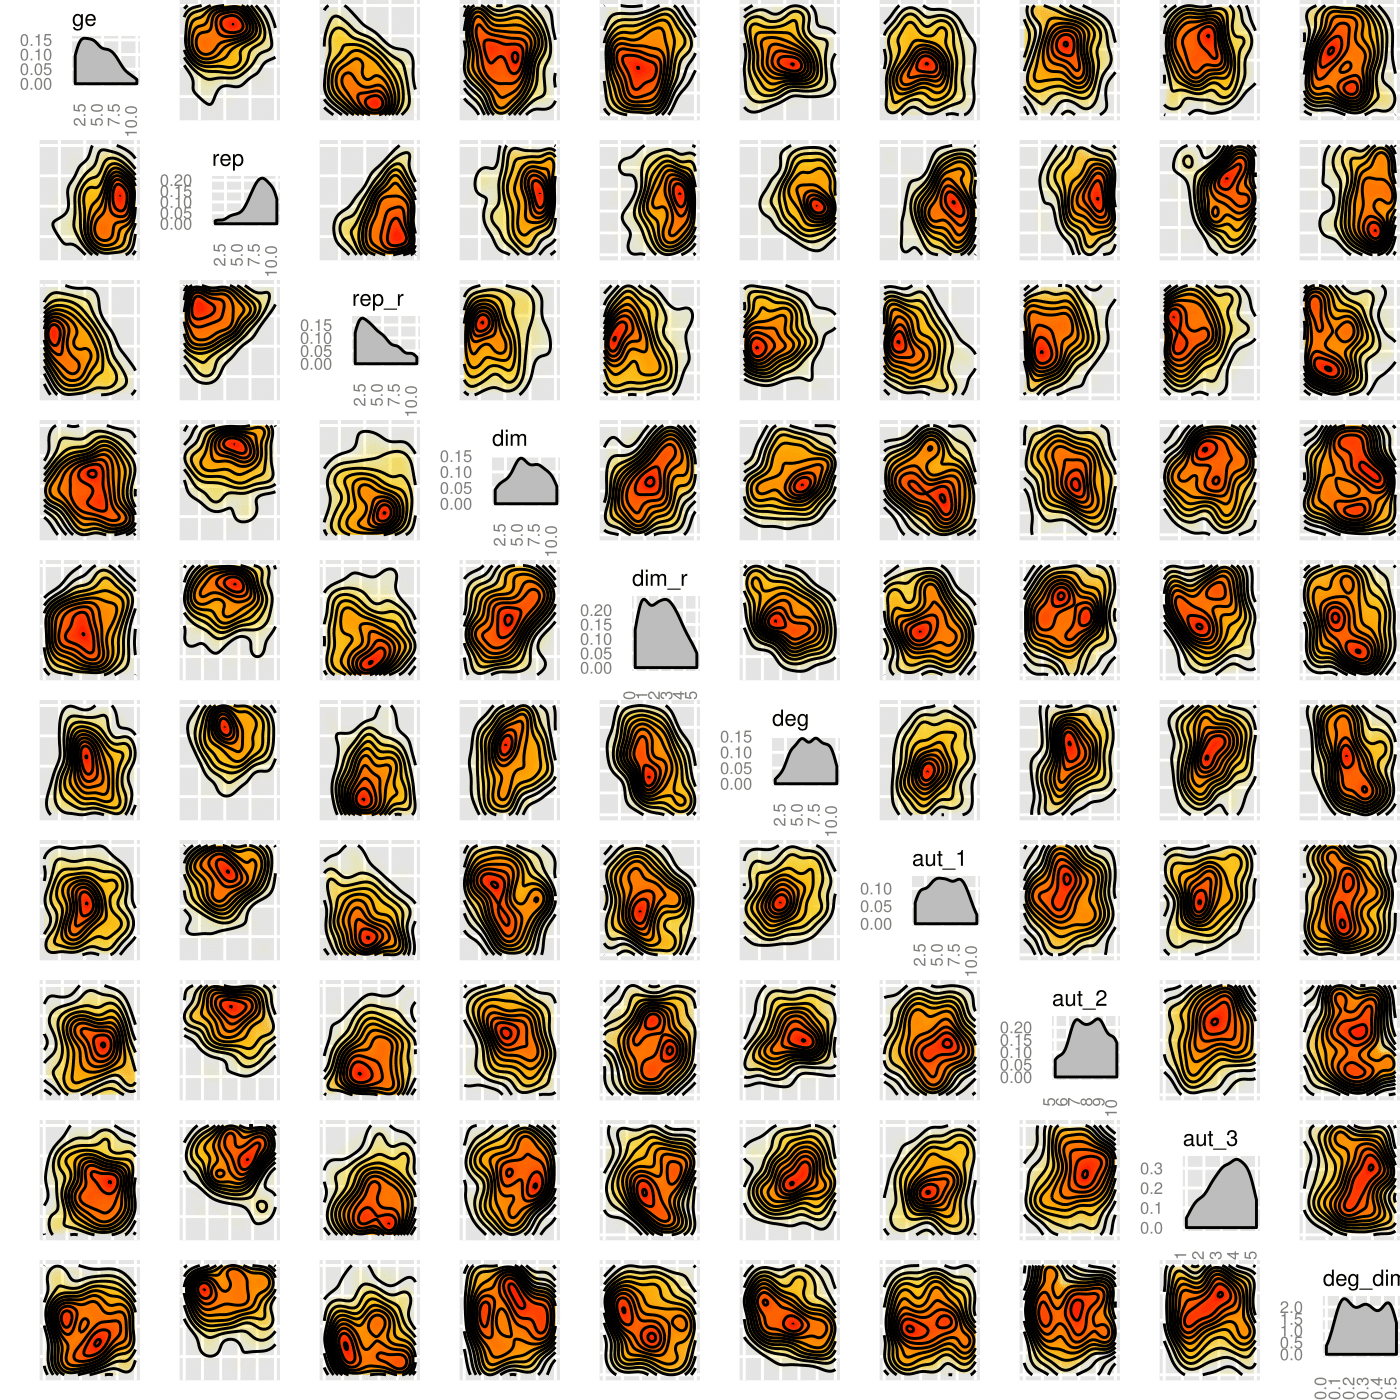
\includegraphics[scale=0.2]{chapterStabilityFinder/mass_action_switches/deterministic/posterior_ma_dp_bi.png}
\caption{The posterior distribution of the Mass action double positive feedback loop switch}
\label{fig:doub_pos}
\end{figure}

\begin{figure}[p]
\centering
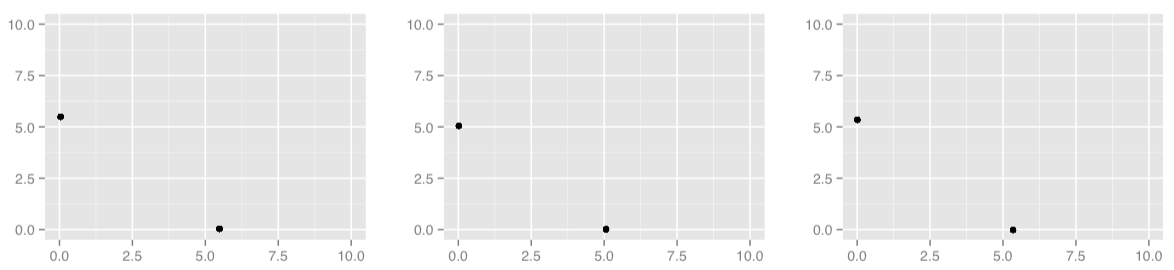
\includegraphics[scale=0.3]{chapterStabilityFinder/mass_action_switches/deterministic/ma_dp_bi_phase_plot.png}
\caption{A sample of the phase plots produced from the final population of the mass action double positive feedback toggle switch.}
\label{fig:det_dp_phase}
\end{figure}

In order to directly compare the robustness of the two models, we used the algorithm outlined in the Methods as a measure of how wide each posterior is given the priors. The results are shown in Figure~\ref{fig:robust_std_doubpos}. 

\begin{figure}[h]
\centering
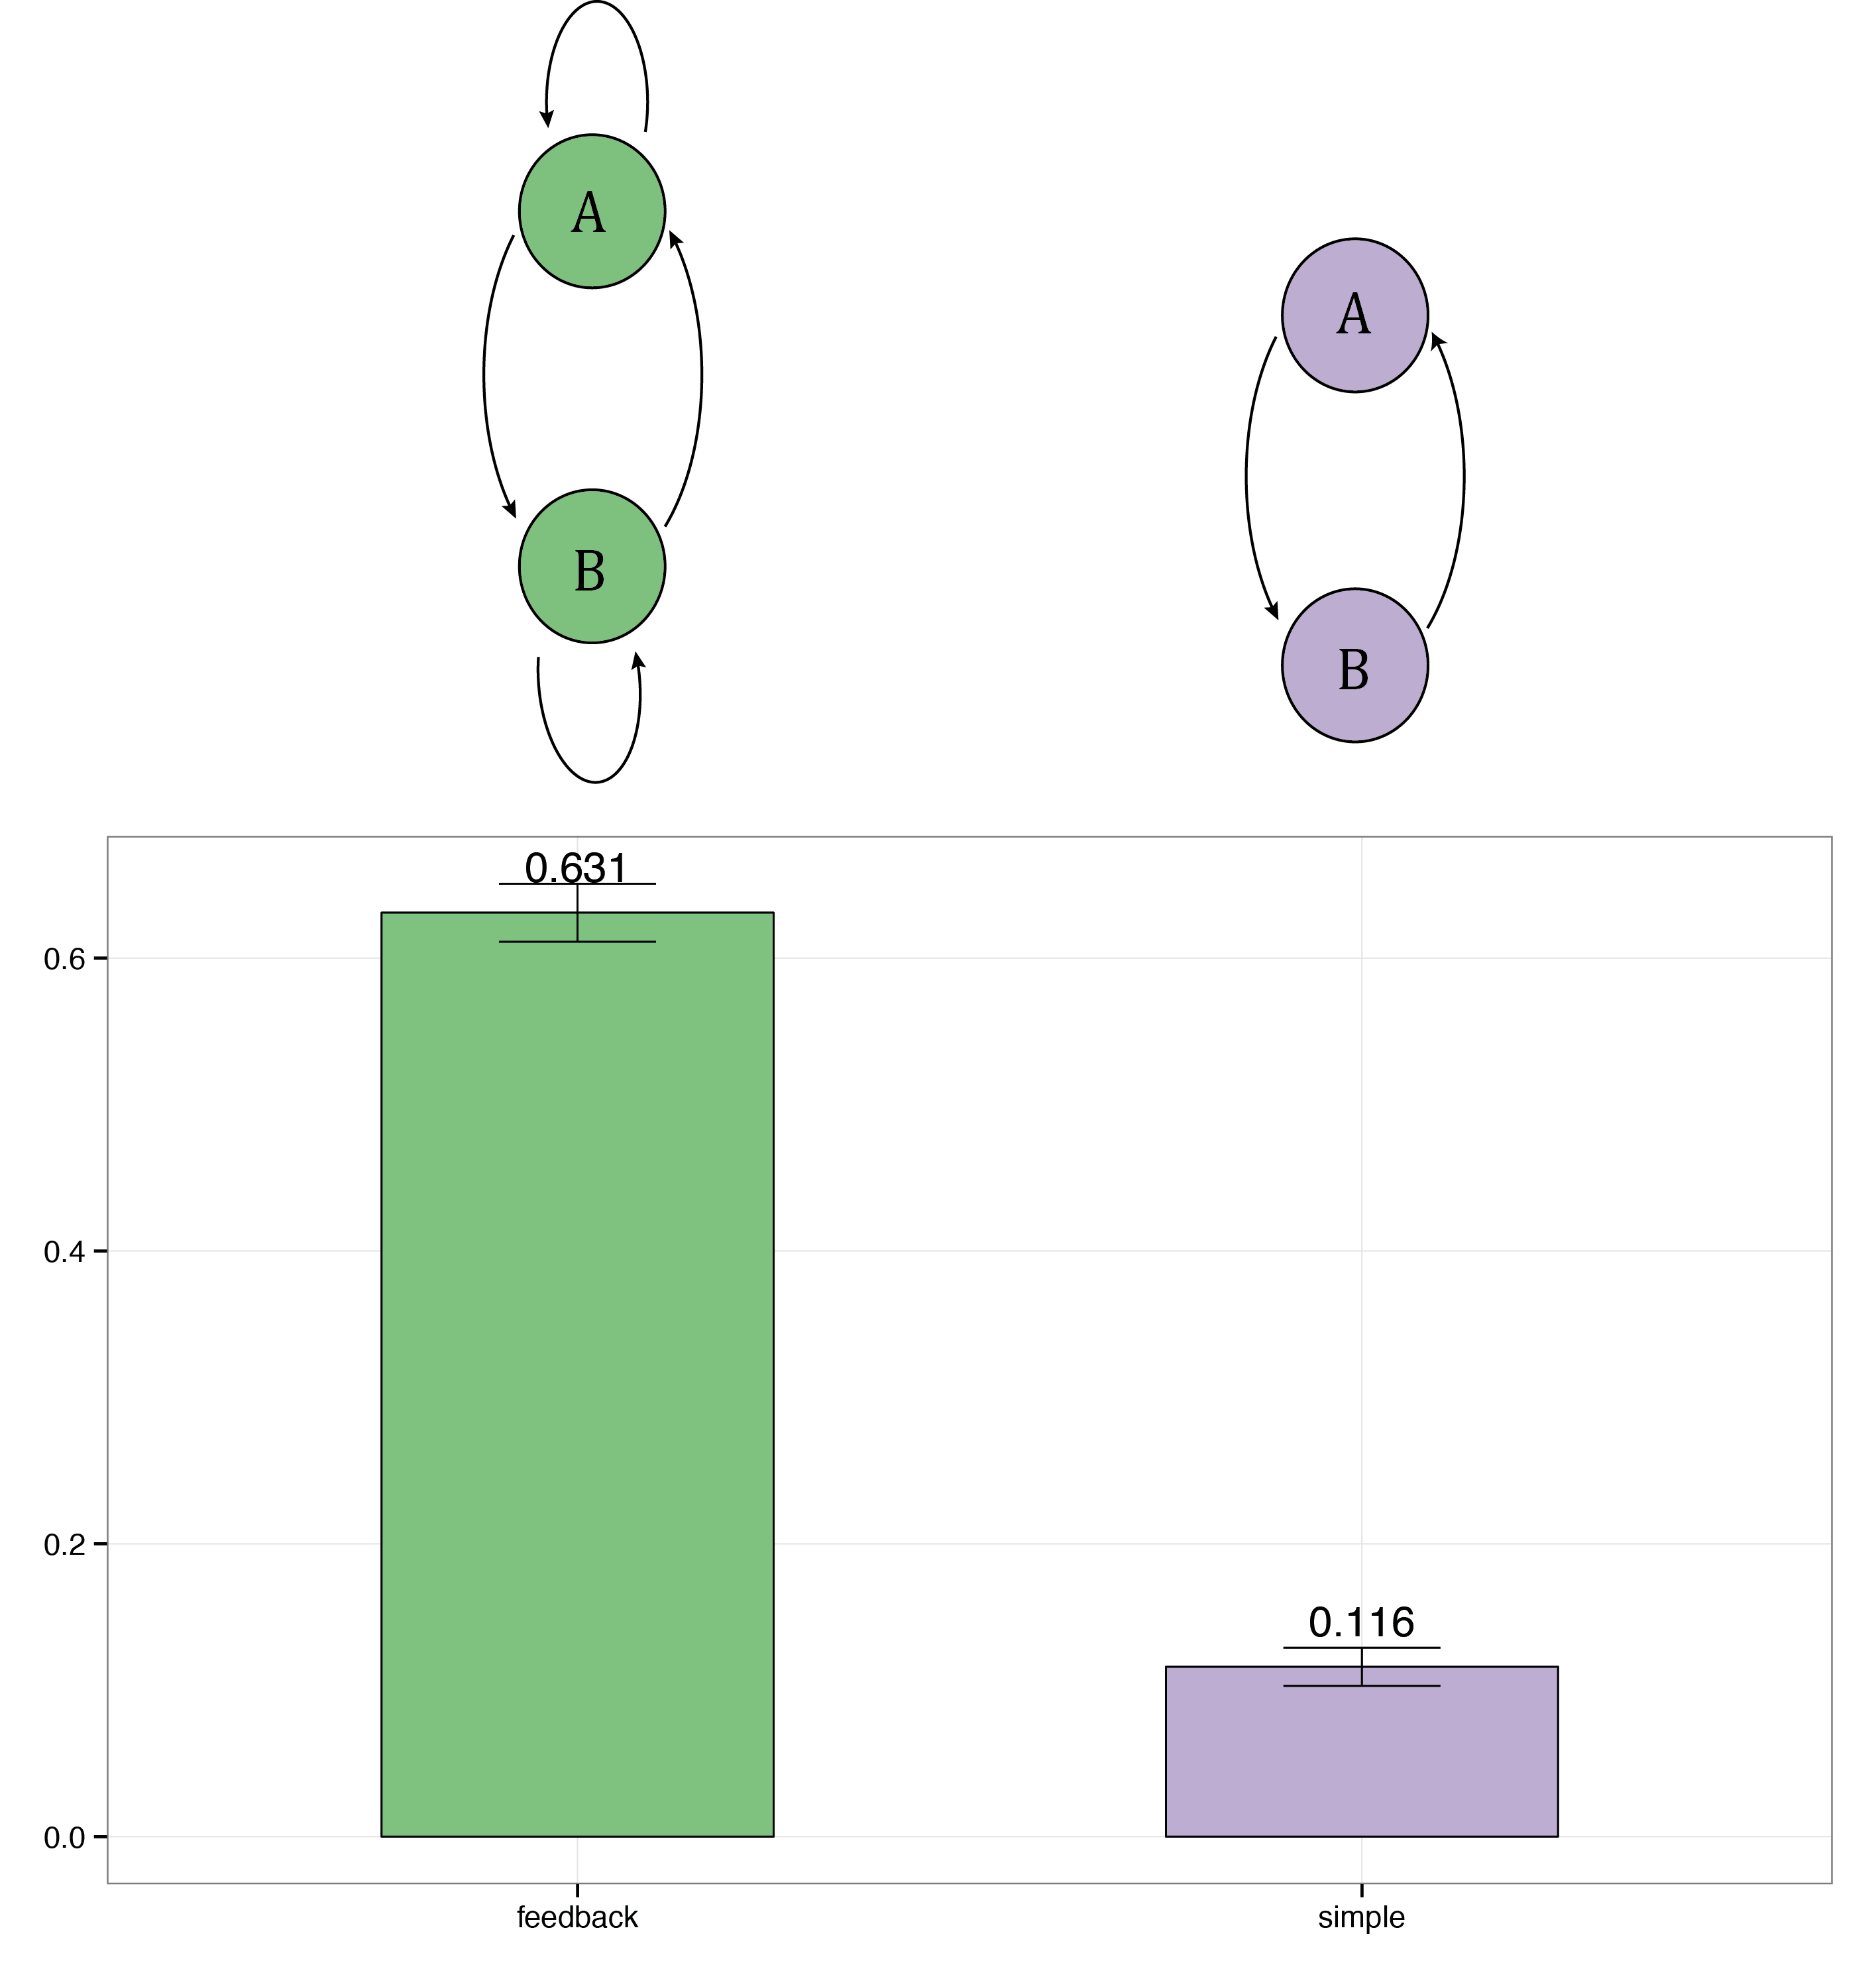
\includegraphics[scale=0.5]{chapterStabilityFinder/mass_action_switches/deterministic/MA_robustness_cartoon.png}
\caption[The robustness of the double positive and the simple switch mass action models]{The switch with double positive autoregulation is more robust to parameter fluctuations that the simple switch. This is evident from the fact that the switch with added feedback has a larger posterior distribution under which it is bistable, compare to the simple switch. Robustness was calculated using a Monte Carlo accept reject algorithm. }
\label{fig:robust_std_doubpos}
\end{figure}
As seen in Figure~\ref{fig:robust_std_doubpos}, the toggle switch with double positive autoregulation is more robust than the simple switch with no feedback. Adding positive feedback loops to the model allows it to be bistable over a greater range of parameter values. This indicates that small fluctuations in parameters in the cellular environment will not flip the switch and thus makes it more suitable for use in synthetic biological applications where spontaneous and undesired switching might be detrimental. 
\clearpage

\subsubsection{Asymmetric switch}
Next, we studied the asymmetric model of the deterministic mass action switch. In this model there are separate gene expression and repression parameters for each gene. The priors used were the ones shown in Table~\ref{tab:asym_cl_det_ma}. The posterior obtained for the classical case is shown in Figure~\ref{fig:asym_det_cl_ma_post} and for the double positive case in Figure~\ref{fig:asym_det_dp_ma_post}.

\begin{table}[htbp]
\centering
\caption{Deterministic asymmetric Mass Action switch priors}
\label{tab:asym_cl_det_ma}
\begin{tabular}{cc}
parameter & range \\
geA & 5-10 \\
repA & 2-10 \\
rep\_r & 0-5 \\
dim & 5-10 \\
dim\_r & 0-5 \\
deg & 1-5 \\
deg\_dim & 0-0.1 \\
geB & 5-10 \\
repB & 2-10 \\
aut\_1 & 1-10\\
aut\_2 & 5-10\\
aut\_3 & 1-5\\
\end{tabular}
\end{table}

\begin{figure*}[htbp]
\begin{center}
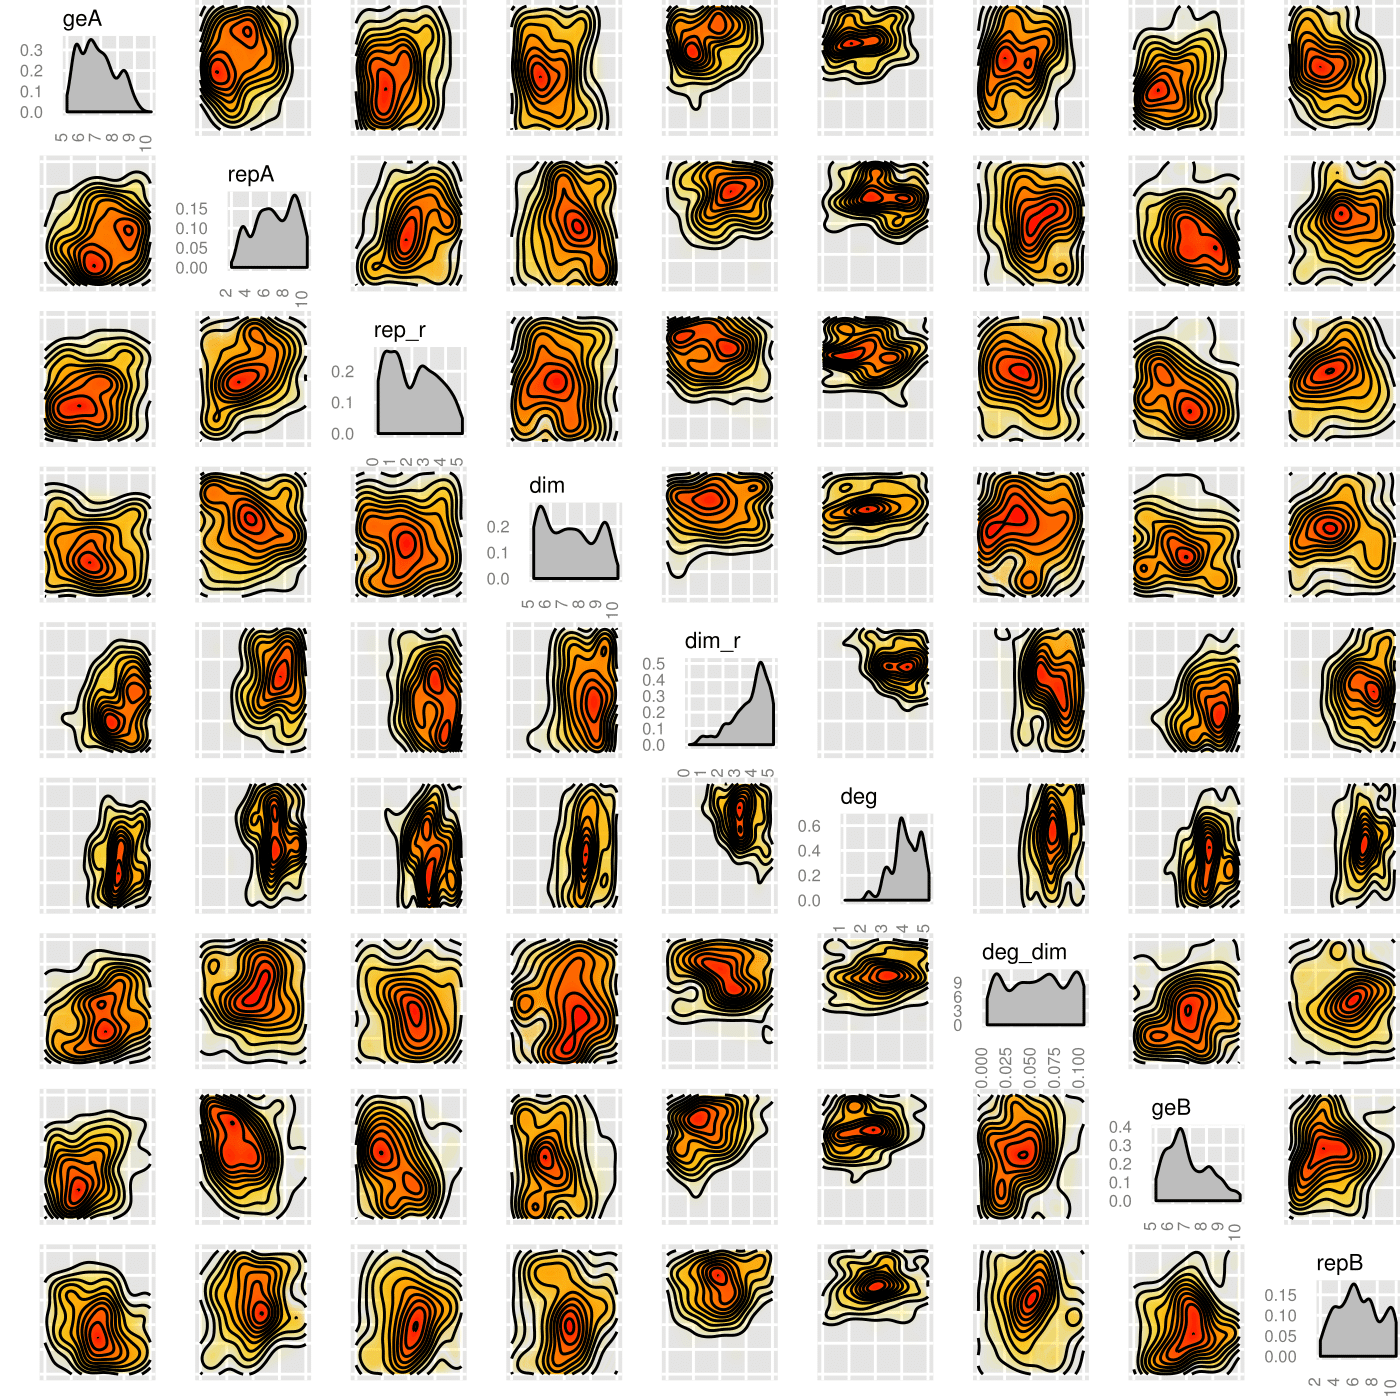
\includegraphics[scale=0.15]{chapterStabilityFinder/mass_action_switches/deterministic/asym/posterior_cl.png}
\caption{Posterior of simple asymmetric deterministic switch}\label{fig:asym_det_cl_ma_post}
\end{center}
\end{figure*}

\begin{figure*}[htbp]
\begin{center}
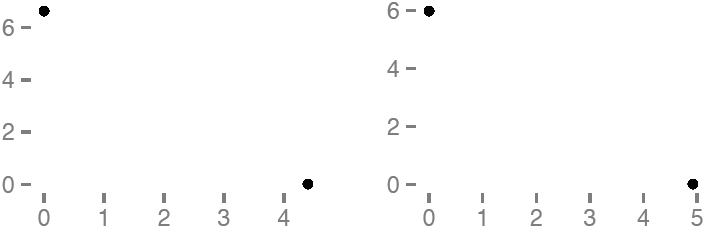
\includegraphics[scale=0.15]{chapterStabilityFinder/mass_action_switches/deterministic/asym/cl_det_phase.png}
\caption{Phase plot of simple asymmetric deterministic switch}\label{fig:asym_det_cl_ma_phase}
\end{center}
\end{figure*}

\begin{figure*}[htbp]
\begin{center}
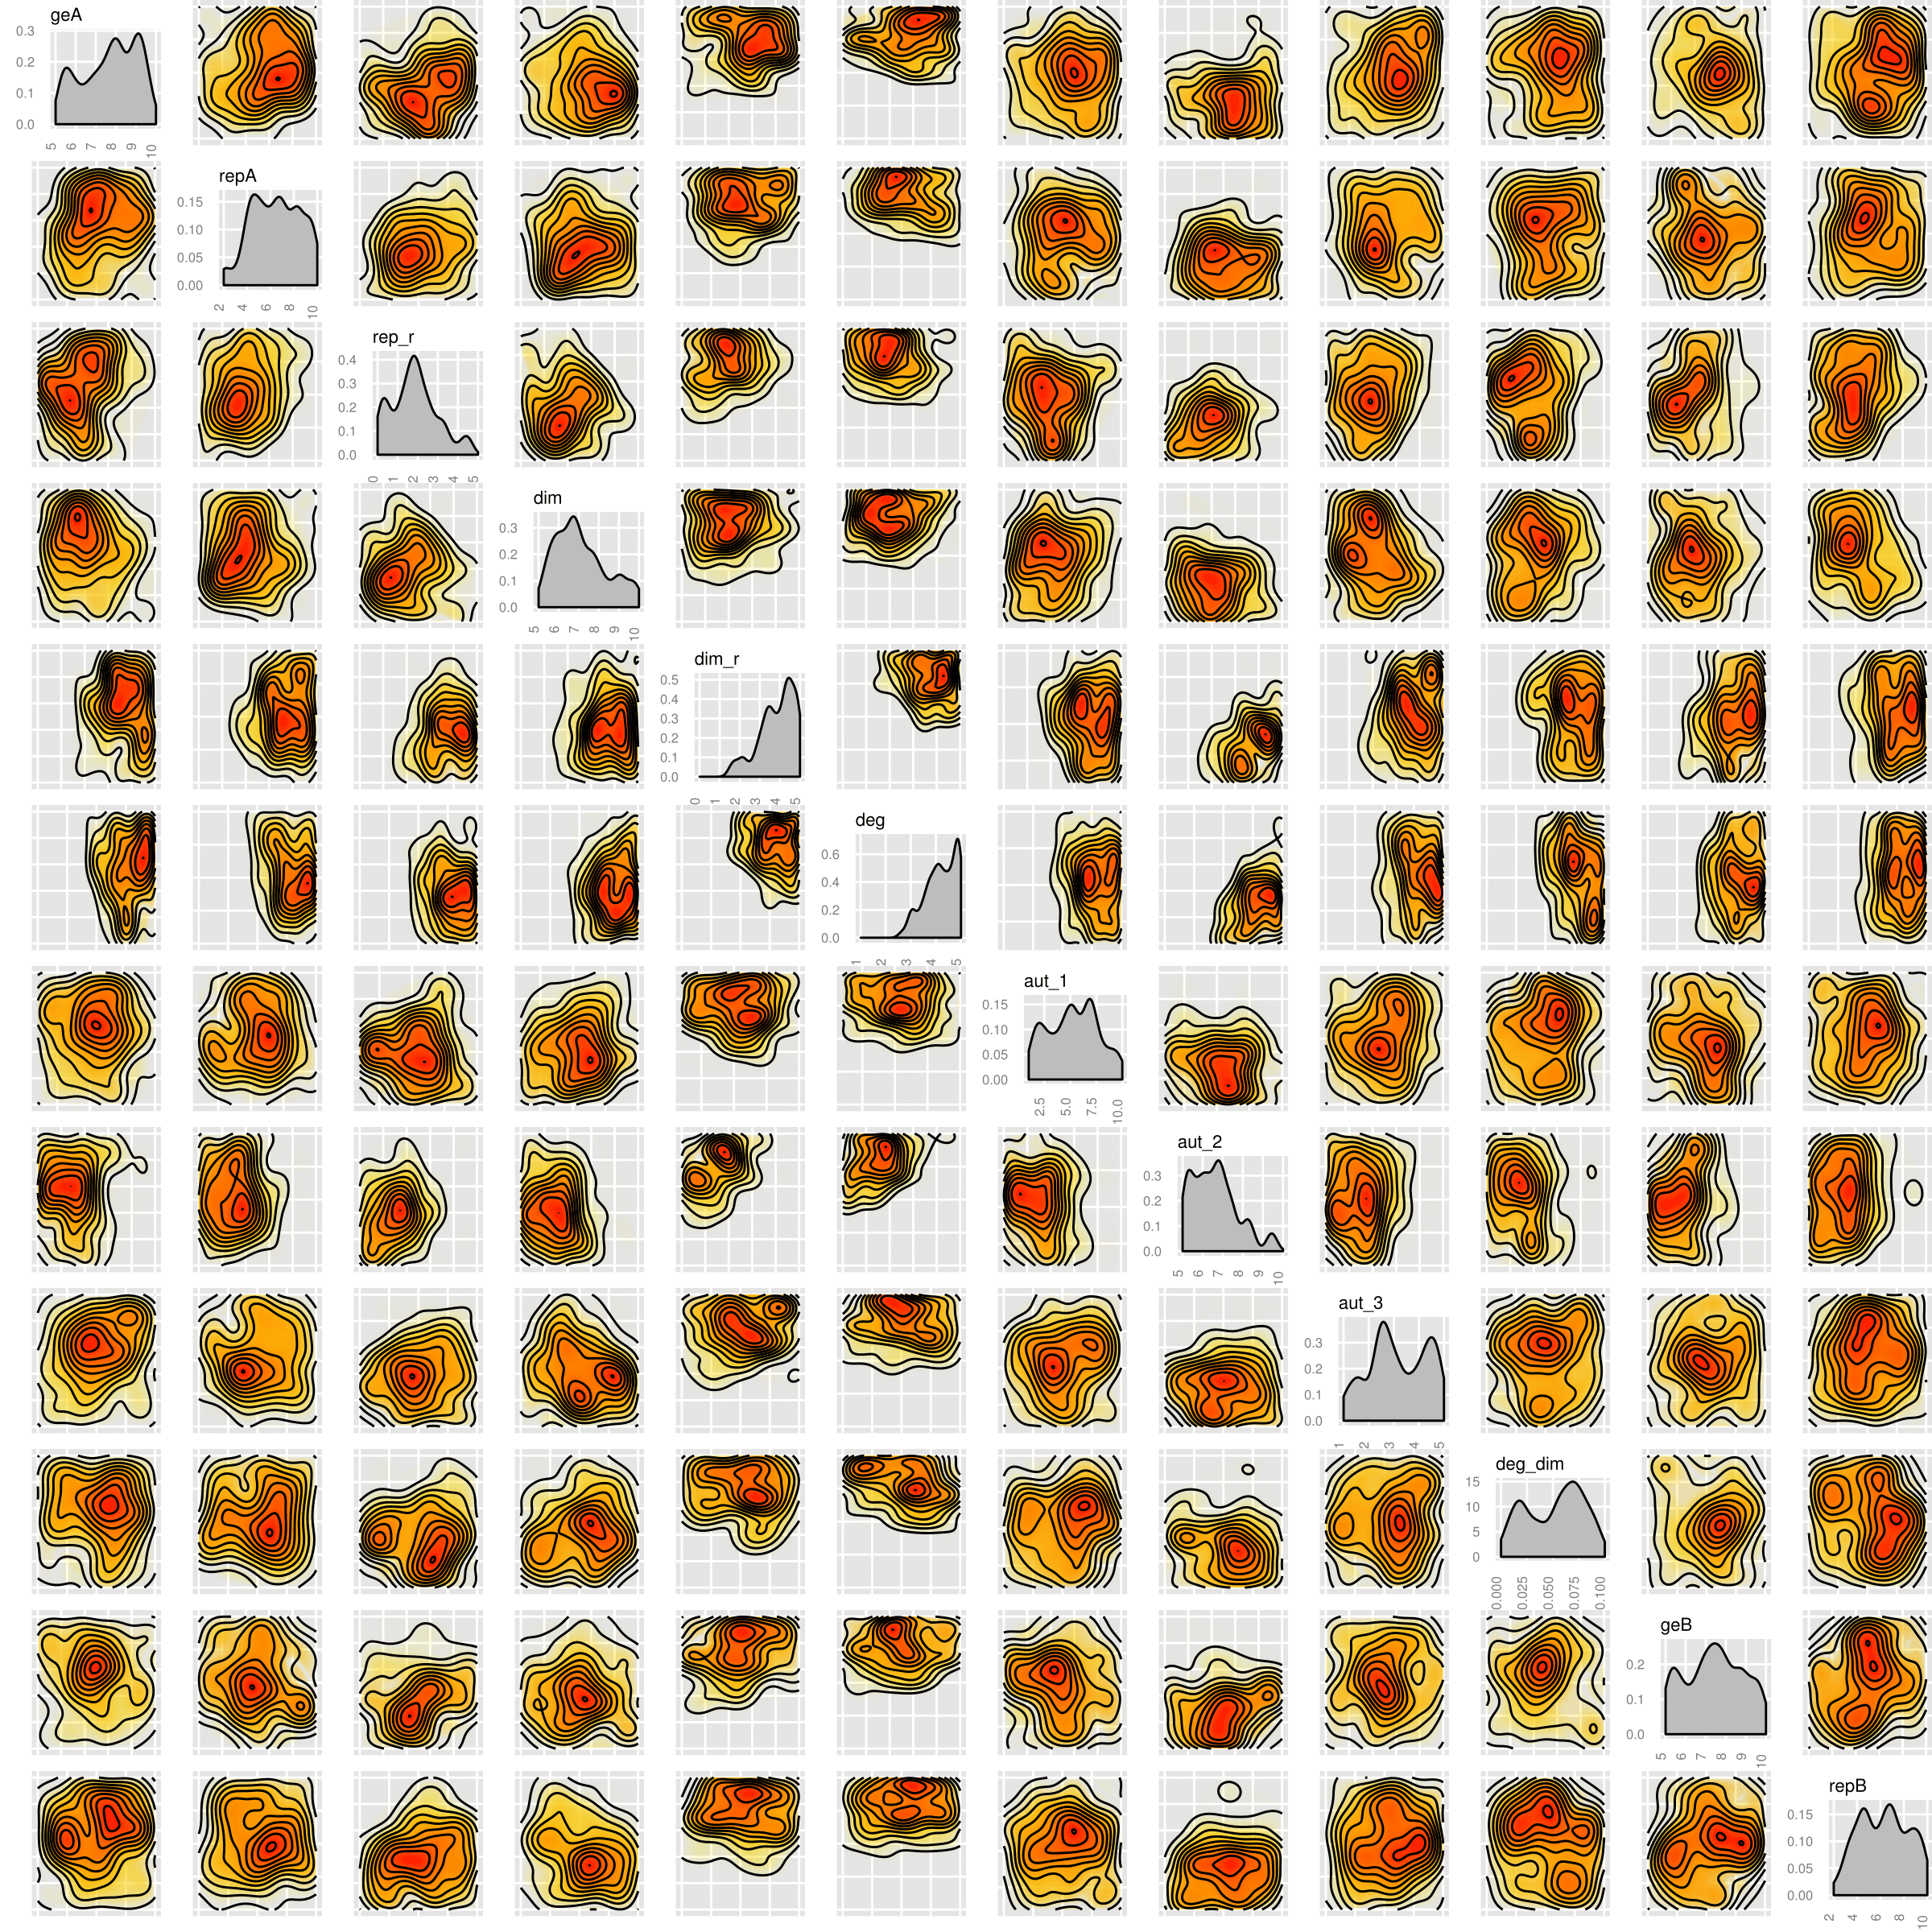
\includegraphics[scale=0.1]{chapterStabilityFinder/mass_action_switches/deterministic/asym/posterior_dp.png}
\caption{Posterior of double positive asymmetric deterministic switch}\label{fig:asym_det_dp_ma_post}
\end{center}
\end{figure*}

\begin{figure*}[htbp]
\begin{center}
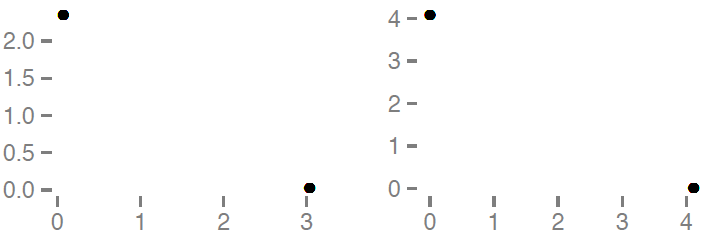
\includegraphics[scale=0.2]{chapterStabilityFinder/mass_action_switches/deterministic/asym/dp_det_phase.png}
\caption{Phase plot of double positive asymmetric deterministic switch}\label{fig:asym_det_dp_ma_phase}
\end{center}
\end{figure*}

\clearpage
\subsubsection{Including transcription and translation}
In order to make these models more realistic, we also separated transcription from translation steps. This is done by adding two parameters to the model to represent translation, while the parameters for gene expression now represent only transcription. The priors used were the ones shown in Table~\ref{tab:asym_cl_rna_det_ma}. The posterior obtained for the classical case is shown in Figure~\ref{fig:asym_det_cl_rna_ma_post} and for the double positive case in Figure~\ref{fig:asym_det_dp_rna_ma_post}.

\begin{table}[htbp]
\centering
\caption{Deterministic asymmetric Mass Action RNA switch priors}
\label{tab:asym_cl_rna_det_ma}
\begin{tabular}{cc}
parameter & range \\
geA & 5-10 \\
trnslA & 0-10 \\
trnslB & 0-10 \\
repA & 2-10 \\
rep\_r & 0-5 \\
dim & 5-10 \\
dim\_r & 0-5 \\
deg & 1-5 \\
deg\_dim & 0-0.1 \\
geB & 5-10 \\
repB & 2-10 \\
aut\_1 & 0-10\\
aut\_2 & 0-10\\
aut\_3 & 0-1\\
\end{tabular}
\end{table}

\begin{figure*}[htbp]
\begin{center}
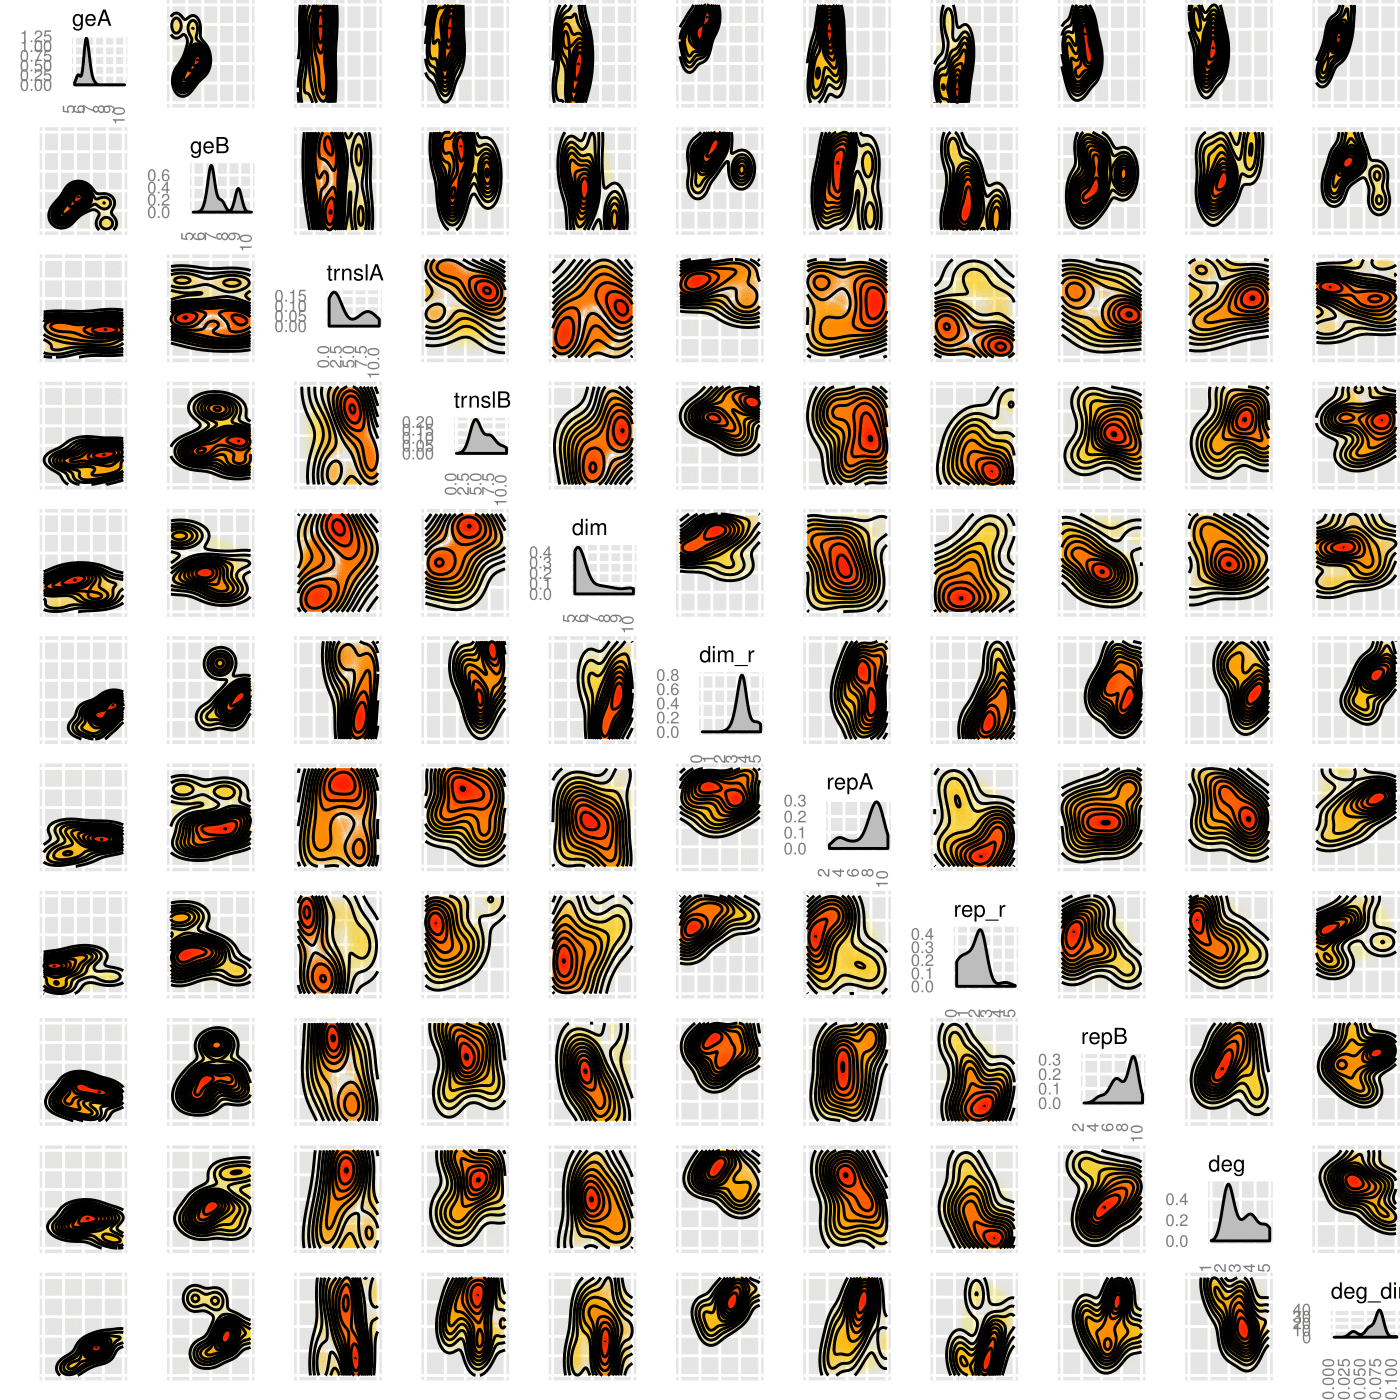
\includegraphics[scale=0.15]{chapterStabilityFinder/mass_action_switches/deterministic/asym/posterior_cl_rna.png}
\caption{Posterior of simple asymmetric RNA deterministic switch}\label{fig:asym_det_cl_rna_ma_post}
\end{center}
\end{figure*}


%\begin{figure*}[htbp]
%\begin{center}
%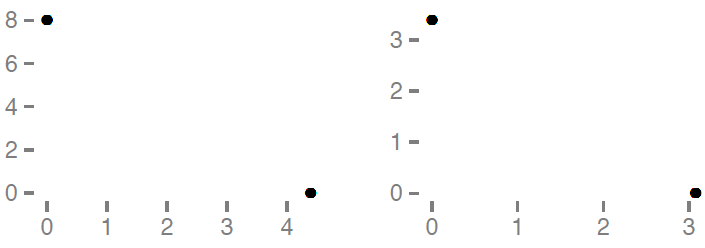
\includegraphics[scale=0.2]{chapterStabilityFinder/mass_action_switches/deterministic/asym/rna_cl_det_phase.png}
%\caption{Phase plot of simple asymmetric RNA deterministic switch}\label{fig:asym_det_cl_rna_ma_phase}
%\end{center}
%\end{figure*}


\begin{figure*}[htbp]
\begin{center}
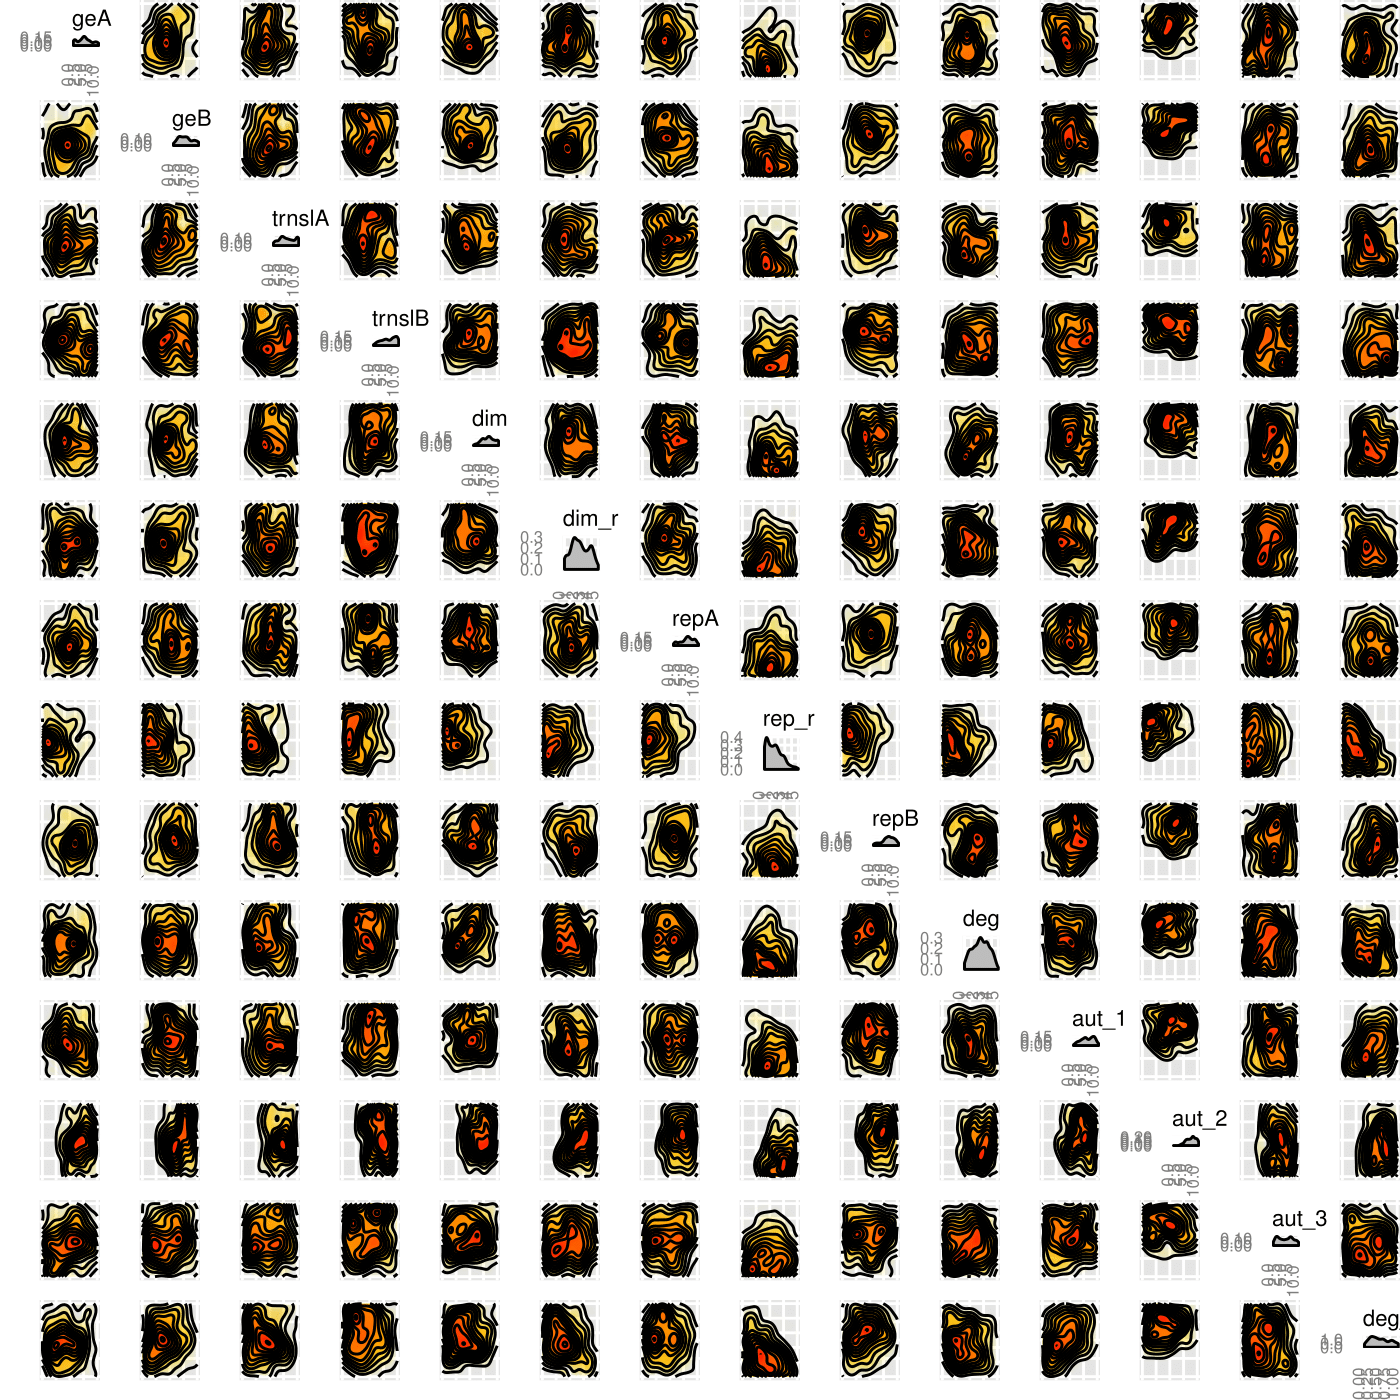
\includegraphics[scale=0.15]{chapterStabilityFinder/mass_action_switches/deterministic/asym/posterior_dp_rna.png}
\caption{Posterior of double positive asymmetric RNA deterministic switch}\label{fig:asym_det_dp_rna_ma_post}
\end{center}
\end{figure*}

%\begin{figure*}[htbp]
%\begin{center}
%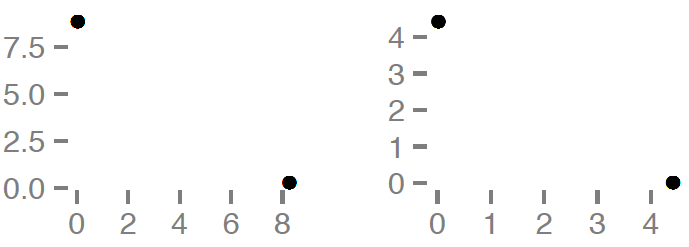
\includegraphics[scale=0.2]{chapterStabilityFinder/mass_action_switches/deterministic/asym/rna_dp_det_phase.png}
%\caption{Phase plot of double positive asymmetric RNA deterministic switch}\label{fig:asym_det_dp_rna_ma_phase}
%\end{center}
%\end{figure*}



\clearpage


%-----%-----%-----%-----%
\subsection{Stochastic case}
\subsubsection{Bistable} 
The model consists of asymetric parameters for gene expression and repression. We search for the parameter space that makes this model tristable. Example phase plots of the resulting tristable switches are shown below. 1000 particles were used in these simulations.


\begin{table}[htbp]
\centering
\caption{priors of bistable switches}
\label{tab:priors_bi}
\begin{tabular}{cc}
parameter & range \\
geA & 0-10 \\
repA & 0-10 \\
rep\_r & 0-10 \\
dim & 7-15 (0-20 in double pos)\\
dim\_r & 0-10 \\
deg & 0-10 \\
deg\_dim & 0-1 \\
geB & 0-10 \\
repB & 0-10 \\
aut\_1 & 0-10 \\
aut\_2 & 0-10 \\
aut\_3 & 0-10
\end{tabular}
\end{table}

\begin{figure*}[htbp]
\begin{center}
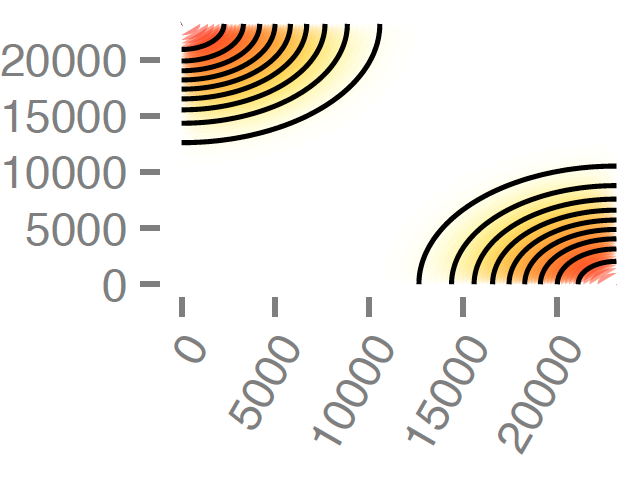
\includegraphics[scale=0.2]{chapterStabilityFinder/mass_action_switches/bi_stoch_images/phase_plt.png}
\caption{Phase plot of the bistable switch.}\label{fig_5}
\end{center}
\end{figure*}

The posterior distributions of the two swicthes:

\begin{figure*}[htbp]
\begin{center}
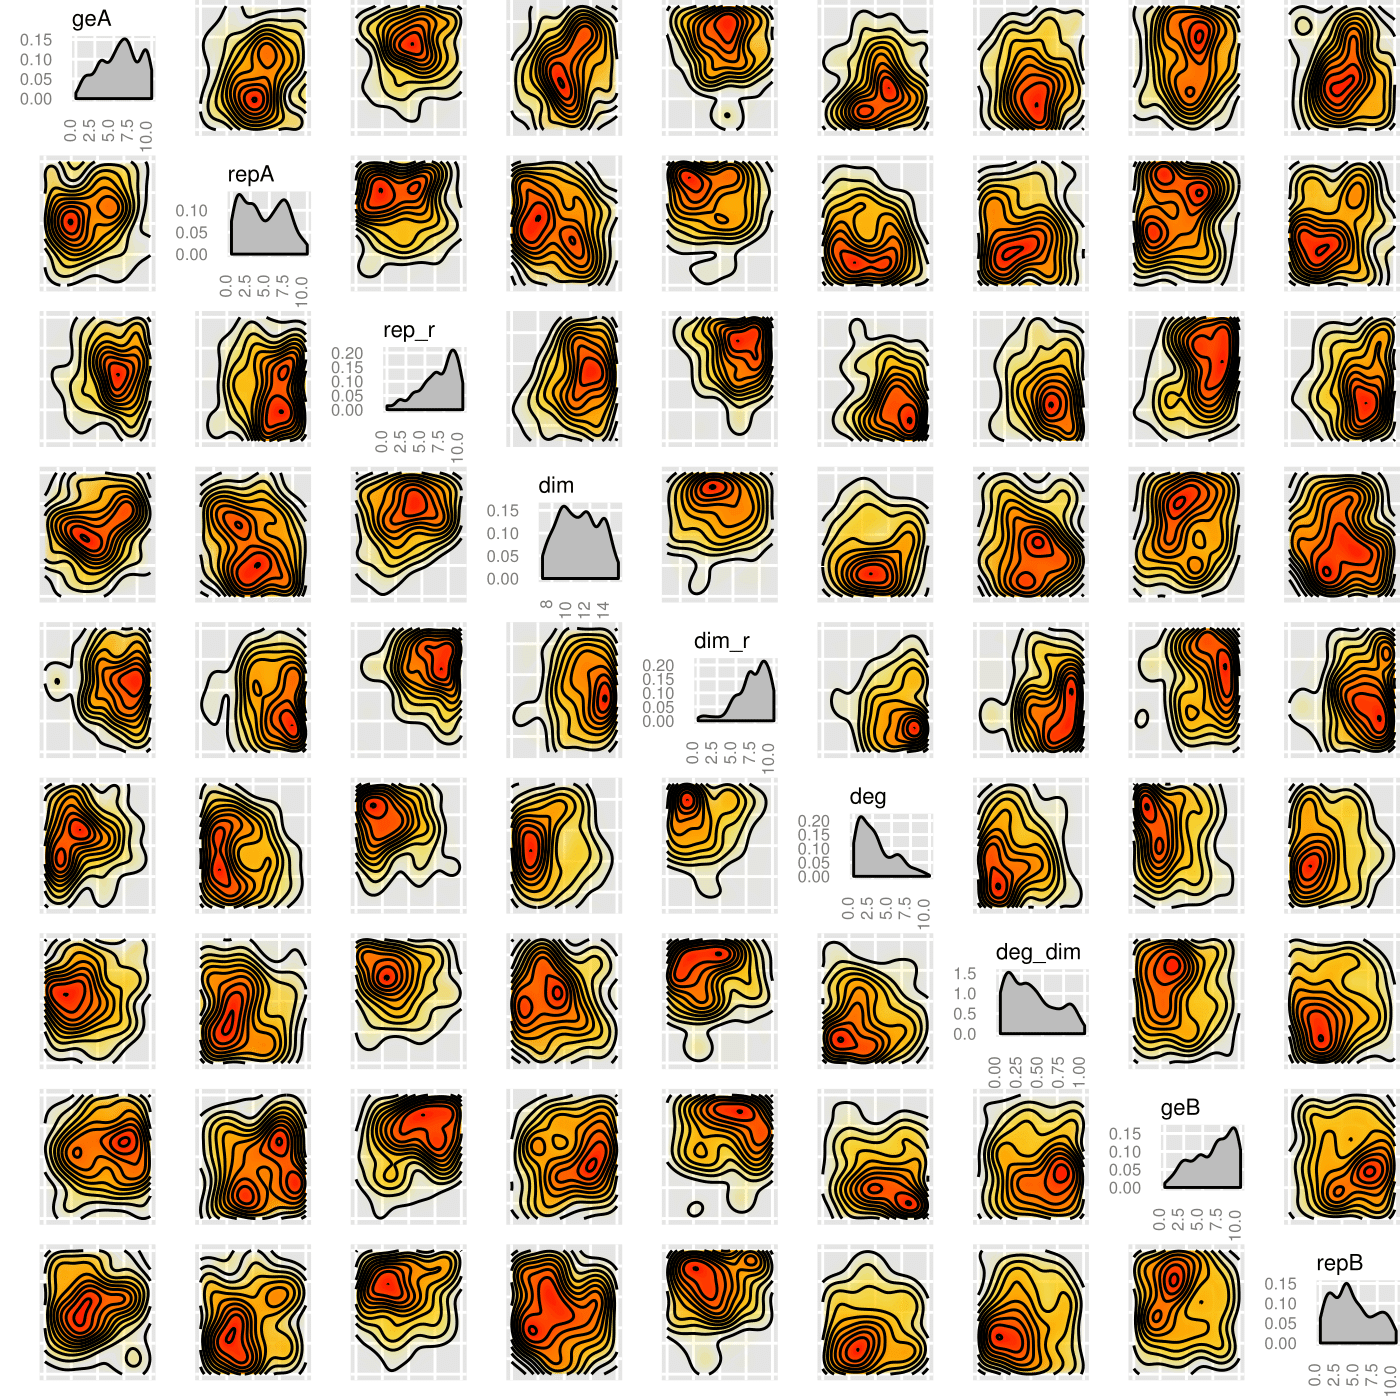
\includegraphics[scale=0.15]{chapterStabilityFinder/mass_action_switches/bi_stoch_images/posterior_std.png}
\caption{Posterior of simple switch}\label{fig_6}
\end{center}
\end{figure*}

\begin{figure*}[htbp]
\begin{center}
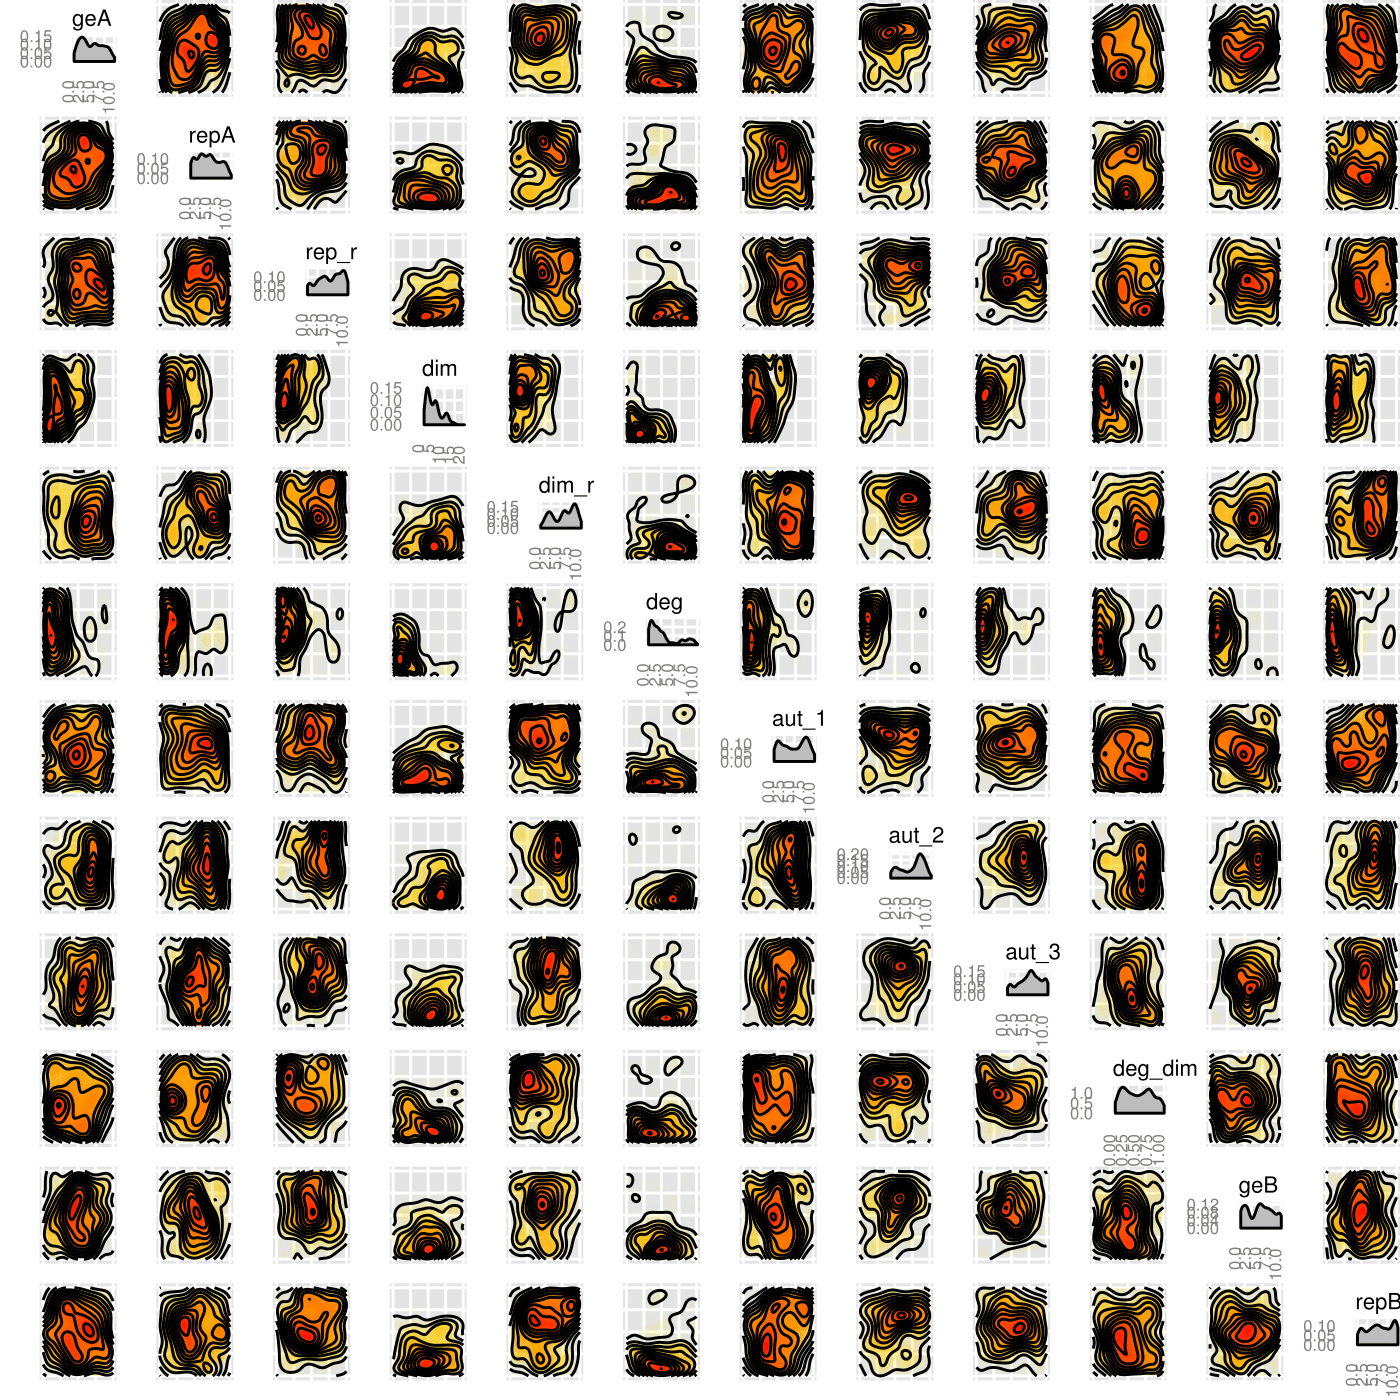
\includegraphics[scale=0.15]{chapterStabilityFinder/mass_action_switches/bi_tri_same_priors/posterior_pos_ab_bi.png}
\caption{Posterior of switch with double positive autoregulation}\label{fig_7}
\end{center}
\end{figure*}

%The robustness of the two switches was compared and no difference was found between the two:
%\newpage
%\begin{figure*}[h!]
%\begin{center}
%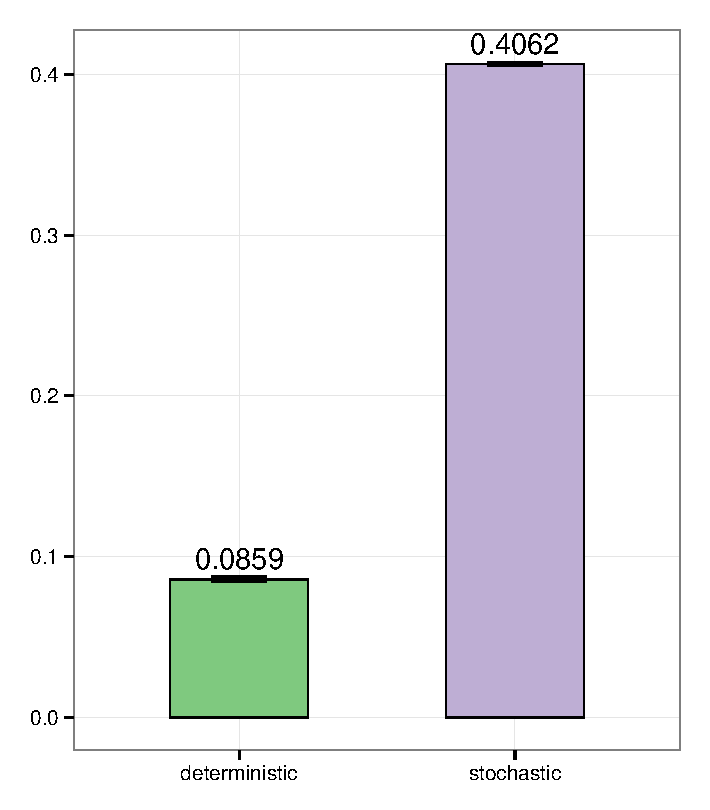
\includegraphics[scale=0.7]{chapterStabilityFinder/mass_action_stochastic_switches/bi_stoch_images/robustness_comparison.pdf}
%\caption{Robustness comparison of the bistable switches. There is no significant diffrence between the two.}\label{fig_8}
%\end{center}
%\end{figure*}

\clearpage
\subsubsection{Tristable}
The model consists of asymmetric parameters for gene expression and repression. We search for the parameter space that makes this model tristable. Example phase plots of the resulting tristable switches are shown below. 1000 particles were used in these simulations.
 
 \begin{table}[htbp]
\centering
\caption{priors of tristable switches}
\label{tab:priors_tri}
\begin{tabular}{cc}
parameter & range \\
geA & 0-10 \\
repA & 0-10 \\
rep\_r & 0-10 \\
dim & 0-20 \\
dim\_r & 0-10 \\
deg & 0-10 \\
deg\_dim & 0-1 \\
geB & 0-10 \\
repB & 0-10 \\
aut\_1 & 0-10 \\
aut\_2 & 0-10 \\
aut\_3 & 0-10
\end{tabular}
\end{table}

\begin{figure*}[h!]
\begin{center}
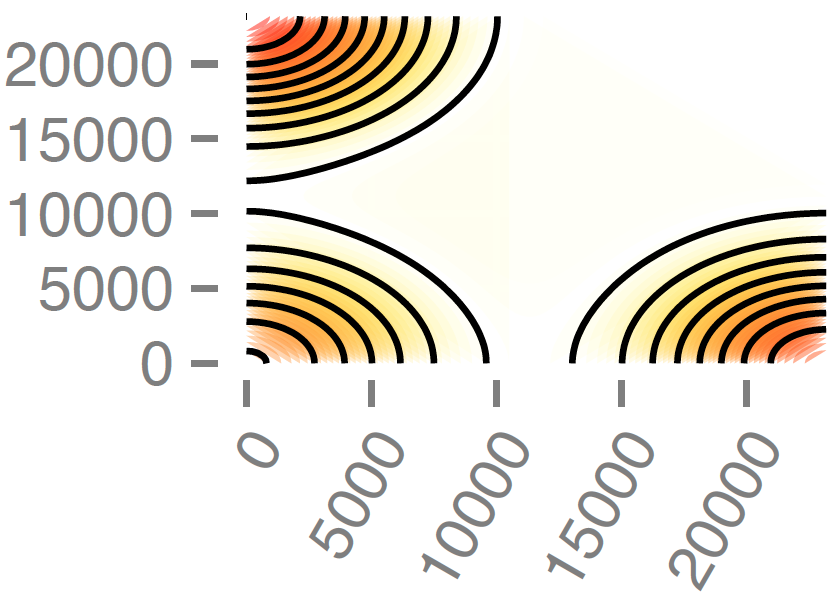
\includegraphics[scale=0.2]{chapterStabilityFinder/mass_action_switches/tri_stoch_images/phase_plot_tri.png}
\caption{Phase plot of the tristable switch.}\label{fig_1}
\end{center}
\end{figure*}

The posterior distributions of the two switches:

\begin{figure*}[htbp]
\begin{center}
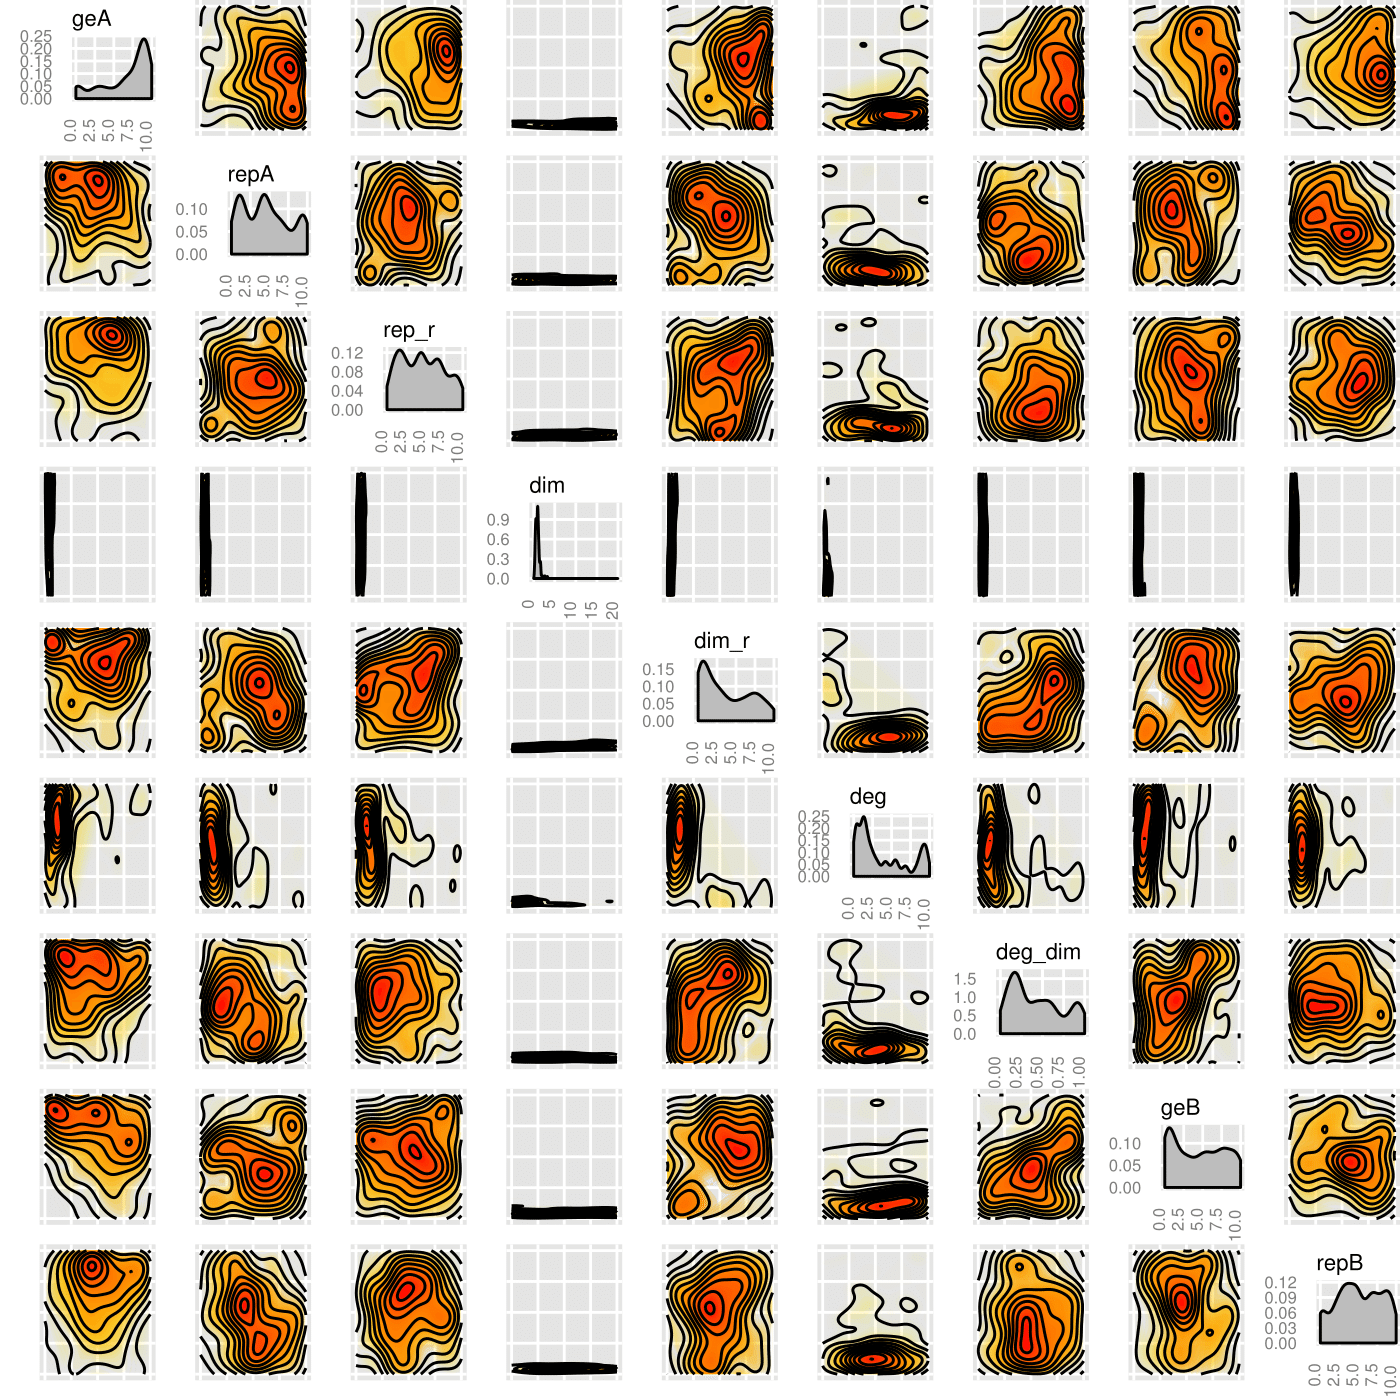
\includegraphics[scale=0.15]{chapterStabilityFinder/mass_action_switches/bi_tri_same_priors/posterior_std_tri.png}
\caption{Posterior of simple switch}\label{fig_2}
\end{center}
\end{figure*}

\begin{figure*}[htbp]
\begin{center}
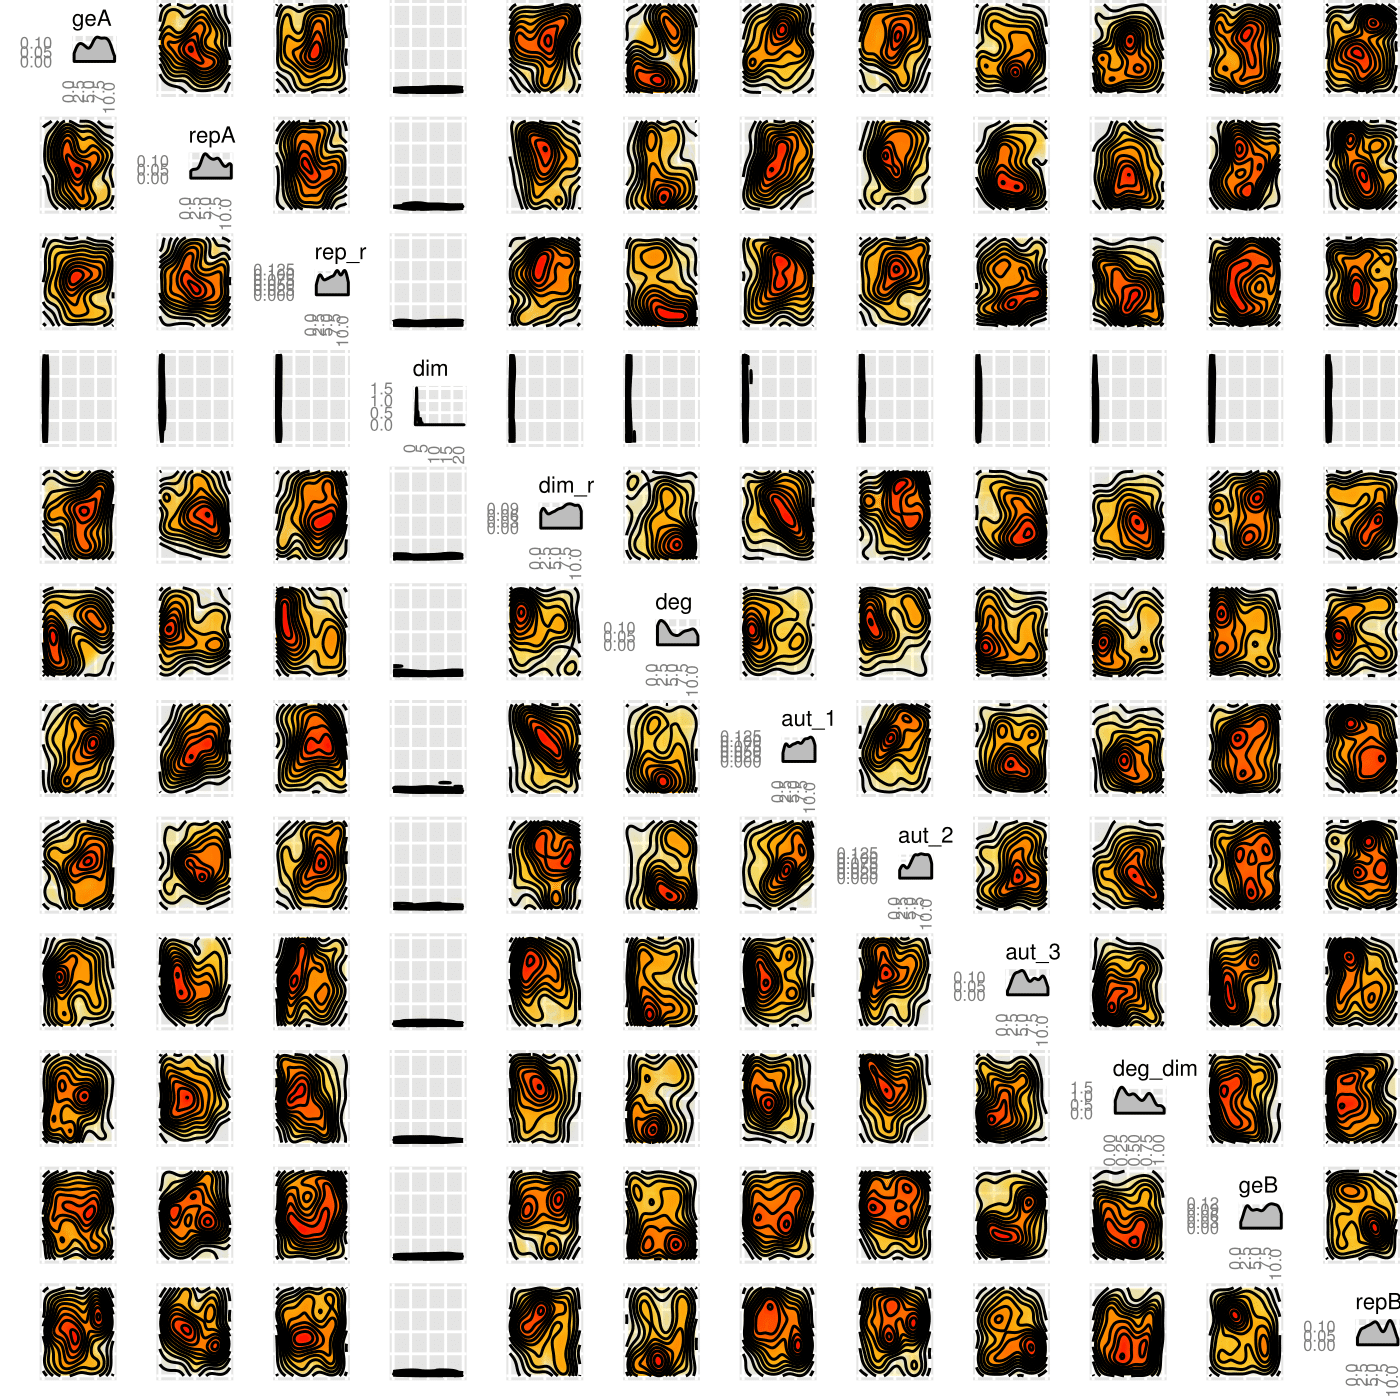
\includegraphics[scale=0.15]{chapterStabilityFinder/mass_action_switches/bi_tri_same_priors/posterior_pos_ab_tri.png}
\caption{Posterior of switch with double positive autoregulation}\label{fig_3}
\end{center}
\end{figure*}
\clearpage
It is clear that in both cases of the switch, the parameter for dimerisation (dim) is very constrained to low values. On the other and, the values for the reverse reaction, the unbinding of dimerisation is not constrained and can take up larger values. 

The robustness of the two switches was compared and no difference was found between the two:

\begin{figure*}[h!]
\begin{center}
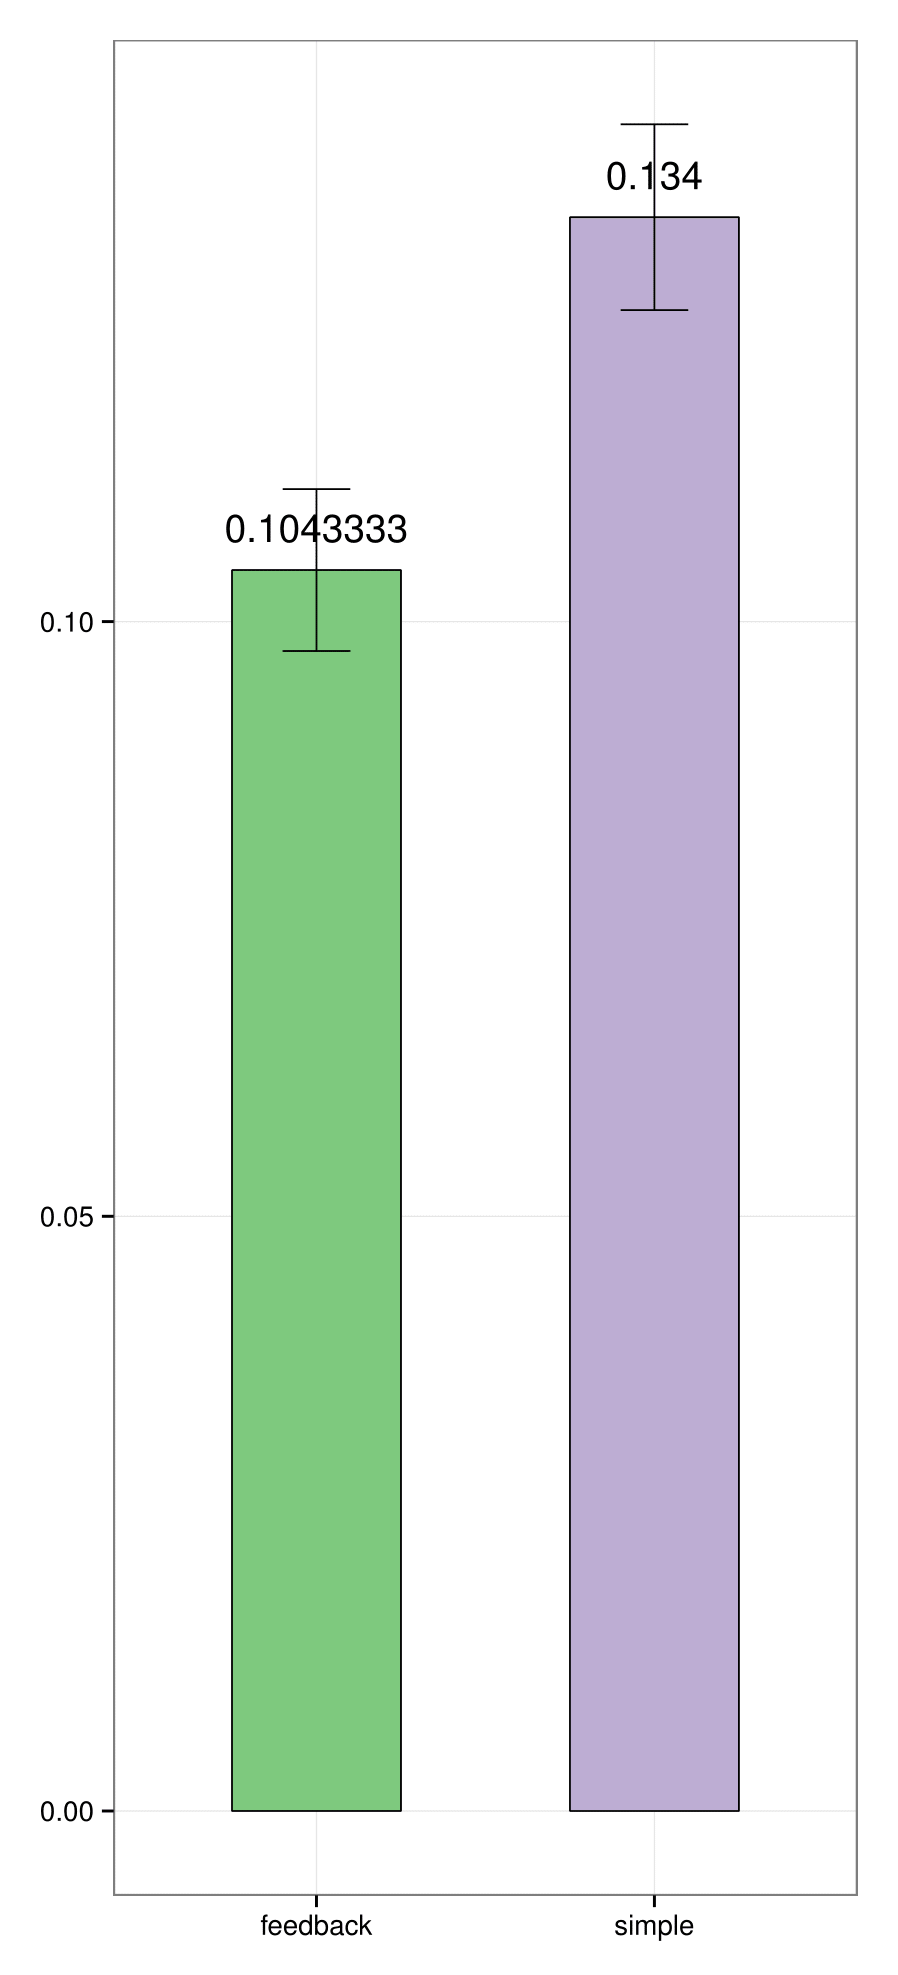
\includegraphics[scale=0.1]{chapterStabilityFinder/mass_action_switches/bi_tri_same_priors/robustness_comparison_tri.png}
\caption{Robustness comparison of the tristable switches. There is no significant difference between the two.}\label{fig_4}
\end{center}
\end{figure*}
\clearpage

\subsubsection{Extracting the design principles of a tristable switch}
Next, we went on to study the design principles that make a switch tristable vs bistable. To do this we implemented an algorithm, as shown in the Appendix. Samples were taken from the posterior distribution of the stochastic double positive mass action tristable switch. Then we separated the values that, for each parameter, were also found in the posterior of the bistable switch. The same procedure was done but taking samples from the bistable posterior and looking for them in the tristable posterior. This can give an indication of the separation of parameter values that can give rise to a bistable vs a tristable switch. The results are shown in Figure ~\ref{fig:design_pr_ma_dp}.

\begin{figure*}[h!]
\begin{center}
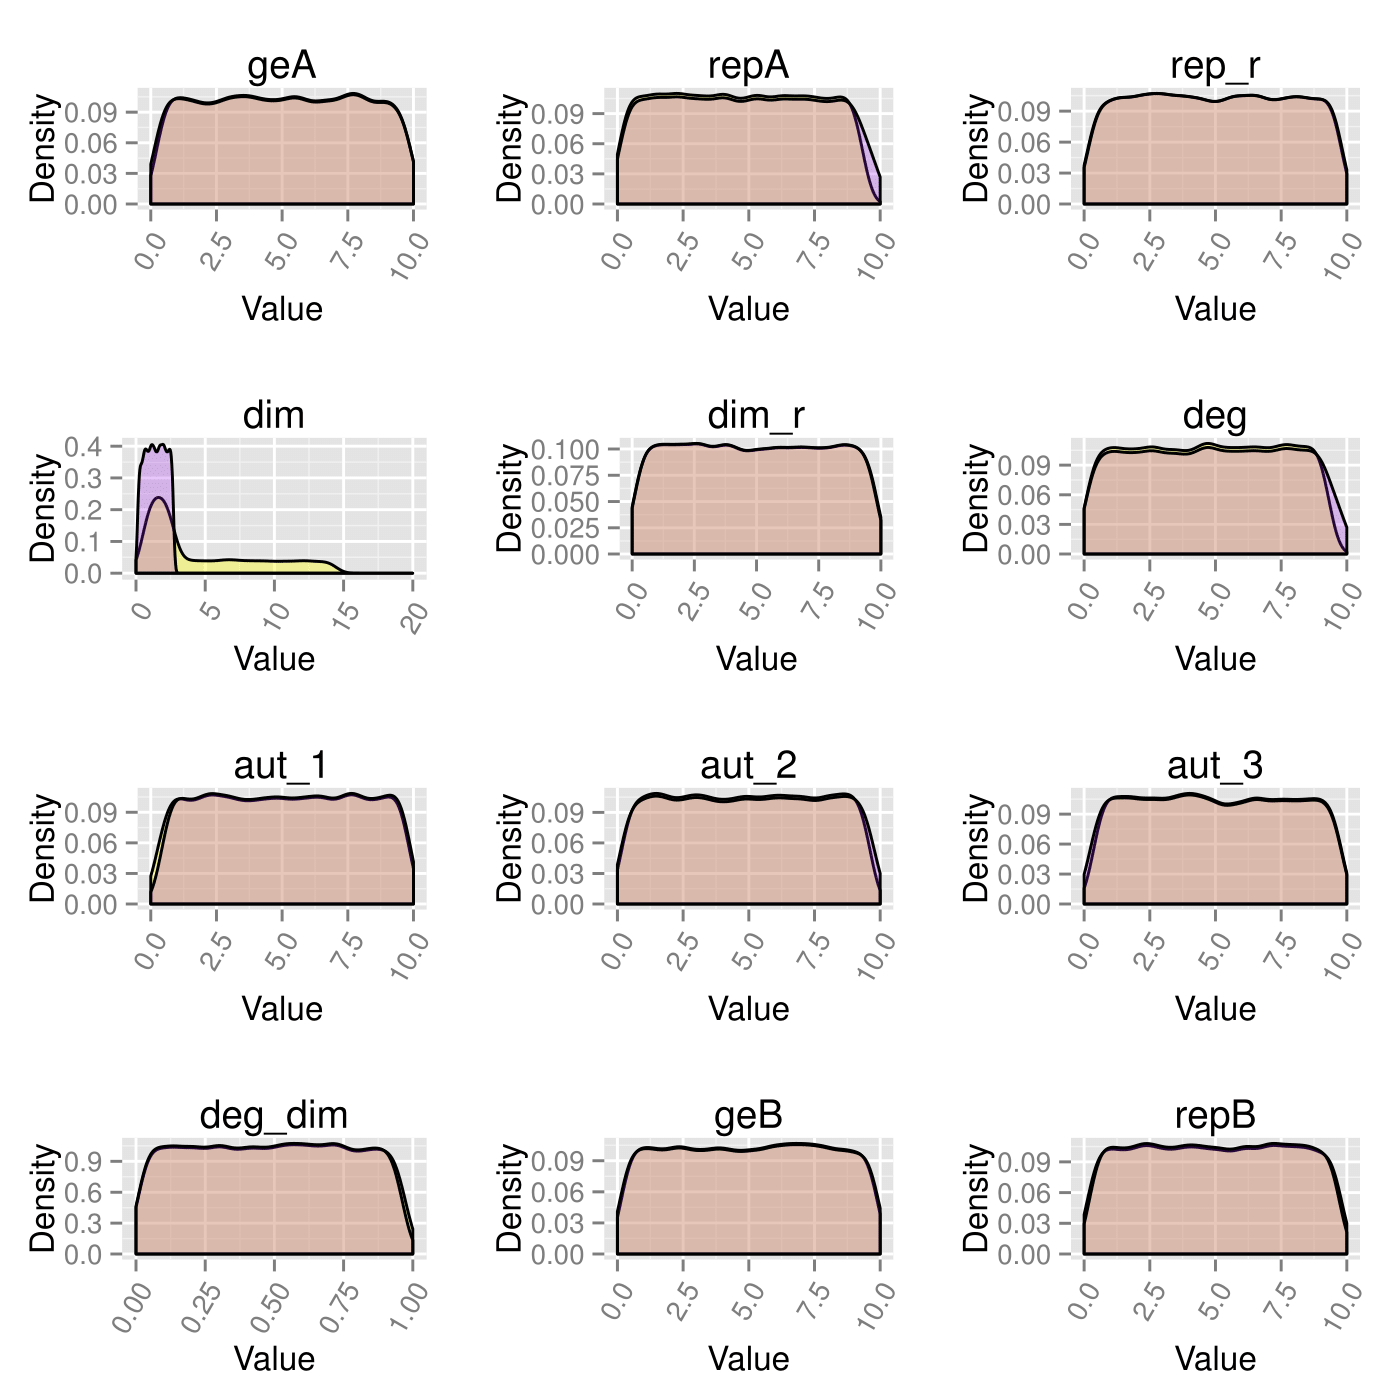
\includegraphics[scale=0.2]{chapterStabilityFinder/mass_action_switches/bi_tri_same_priors/design_principles_pos_ab.png}
\caption{Extracting the tristable versus bistable switch design principles. Yellow represents a bistable switch and red a tristable}\label{fig:design_pr_ma_dp}
\end{center}
\end{figure*}

From the above results it can be seen that the only parameter that is different in the two switches is the one representing dimerisation (dim). For both a bistable and a tristable switch the value for dim must be small, although this condition is more constrained in a tristable switch.

%\section{Discussion}

Here we presented a methodology, StabilityFinder, which can identify the region of parameter space that can produce the stability of choice. We demonstrated its use on some known models and extracted stability and robustness information from them. We compared the stability profile of the Gardner toggle switch when modelled deterministically and stochastically in order to uncover the differences that arise from the addition of noise in the modelling.% We found that the stochastic model showed increased robustness to noise.

We then applied StabilityFinder to the Lu switches in order to uncover the design principles that make a switch bistable versus tristable. %We found that the gene expression parameters were critical for making a tristable switch bistable. This would be in agreement with the dynamics of a tristable switch, in which the third steady state occurs when there is a deadlock situation between the two proteins. When there are small numbers of both proteins involved, one represses the production of the other resulting in both promoters being repressed \autocite{Ma:2012dt}. Given our result we can extrapolate that a higher rate of protein production eliminates the possibility of this deadlock situation happening. Once a promoter is free to produce protein it will produce it in a fast enough rate so that that protein dominates the system and represses the antagonizing promoter before it has the chance to repress it. This dynamic would explain the fact that when all the priors remained the same but gene expression was increased by an order of magnitude, the tristable switch became bistable. 

We also applied StabilityFinder to a synthetic biology design problem. We used two models of the switch, one simple model consisting of two mutually repressive transcription factors and a model with added double positive auto-regulation. Comparing the two models, both capable of bistable behaviour, using StabilityFinder we found that the model with added double positive feedback loops is more robust to parameter fluctuations. This makes it a better candidate for building new synthetic devices based on the toggle switch design. We identified the parameter region within which this models are bistable, information that is important when building such a device in the lab. In the future, by selecting the system components accordingly, the parameter values can be adjusted \textit{in vivo}. For example, the parameter value corresponding to the translation initiation rate can be chosen by selecting the appropriate RBS sequence which given a nucleotide sequence will produce the desired rate \autocite{Holtz:2010bm}, a method developed by Salis \autocite{Salis:2009gk}. Another method to tweak the parameter values \textit{in vivo} is to select the promoter to have the strength corresponding to the levels of gene expression and repression desired. Activity of each promoter can be measured and standardised \autocite{Kelly:2009bj} making this process possible. For a system requiring more than one promoter, these can be efficiently selected from a promoter library using a genetic algorithm created by \textcite{Wu:2011bq}. These standardised interchangeable components with known sequence and activity are what synthetic biology classes as BioBricks \autocite{Kelly:2009bj,Canton:2008fv}. These can be selected and used to construct a desired system and replicate the parameter values found using StabilityFinder.

The methodology we presented here can be applied to a variety of problems as demonstrated. It can be applied to any problem of finding the parameter values that can produce a desired stability between two species. It can be used to design new systems of desired stability and help identify the appropriate parts to use by identifying the rates within which these parts need to operate. It can also be used to examine existing systems and give an insight on the underlying mechanisms that allow for the given stability to occur. 





%%  Characterising the toggle switch -----------------%%
\mainmatter*
\chapter{Bayesian model fitting applied to flow cytometry data}
\section{Circuit overview}

\section{Growth rate investigation}

\section{Flipping the switch - promoter sensitivity}

\section{Time course data}

\section{Model fitting}

\section{Introduction}
\section{Methods}

\begin{algorithm}[htbp]
\label{alg:abc-flow}
\caption{ABC-Flow}
 \begin{algorithmic}[1]
 	\Statex
 \State Read input file
	\If{ABC-Rejection}
 		\State Sample from priors
 		\State Simulate model
 		\State Convert signal to intensity
 		\State Measure distance to data
		\State Reject particles if d $\textgreater$ $\epsilon$.
 		\If{number of accepted particles == number of particles}
 			\State Exit
 		\Else
 			\State Return to step 3.
 		\EndIf
 	\EndIf
 	
 	\Statex
 	\If{ABC-SMC}
	\State Initialise $\epsilon$ 
	\Let{population p}{1}
	\If{p $= 1$}
		\State Sample particles ($\theta$) from priors
		\Else
			\State Sample particles from previous population
			\State Perturb each particle by $\pm$ half the range of the previous population (j) to obtain new perturbed population (i).
	\EndIf
	\State Simulate model
	\State Convert signal to intensity
	\State Measure distance to data
	\State Reject particles if d $\textgreater$ $\epsilon$.
    \State Calculate weight for each accepted $\theta$
	\State $w_{t}^{(i)} = \begin{cases} 1, & \mbox{if } p = 0 \\\frac{\pi(\theta_{t}^{(i)})}{\sum_{j=1}^N w_{t-1}^{(j)} K_{t}(\theta_{t-1}^{(j)}, \theta_{t}^{(i)})}, & \mbox{if } p \geq  0. \end{cases}$
	\State Normalise weights
	\Repeat{ steps 17 - 29} \Until{$\epsilon \leq \epsilon_T$}
	\EndIf
  \end{algorithmic}
\end{algorithm}
\clearpage

\section{Results}

\subsection{Distance Calculations}

\begin{algorithm}[htbp]
\label{alg:dist}
\caption{Distance calculation}
 \begin{algorithmic}[1]
    \Statex
	\Let {Grid}{min(data):max(data):ngrid} 
	\State kD = kernel density estimation(data)
	\State kS = kernel density estimation(simulations)
	\State fD = kD(xx)
	\State fS = kS(xx)    
	\State $d = \sum((fD-fS)^2)$
  \end{algorithmic}
\end{algorithm}

    
%\begin{algorithm}[htbp]
%\label{alg:2Ddist}
%\caption{2D distance calculation}
% \begin{algorithmic}[1]
%    \Statex
%	\Let {Grid}{xmin(data):xmax(data):ngrid, ymin(data):ymax(data):ngrid} 
%	\State kD = kernel density estimtion(data)
%	\State kS = kernel density estimtion(simulations)
%	\State fD = kD(xx)
%	\State fS = kS(xx)    
%	\State $d = \sum((fD-fS)^2)$
%  \end{algorithmic}
%\end{algorithm}


\subsection{Comparing 1D and 2D distances}
In order to compare the 1D and 2D fitting to the data in ABC-Flow, we must first find out how comparable the distance measures are. Here we  simulate two normal distributions, with identical mu and sigma, and calculate the distance between the two using the distance measure used in ABC-Flow. Doing this 1000 times, we then plot the distribution of epsilon. By doing that we can calculate the variance of the epsilon distribution, and find out the error that can be expected when measuring the distance in ABC-Flow. By doing that in 1D and in 2D we can compare the epsilon variances. 

\begin{figure}[htbp]
\centering
\includegraphics[scale=0.3]{chapterABCFlow/images/normal_sigma_example.png}
\caption{Comparing 1D and 2D distributions.}
\label{fig:normal_example}
\end{figure}



 \subsubsection{Normal distribution}
Here, we simulate two normal distributions, with $\mu=0$ and $\sigma=1$ 1000 times and measure the distance. In the 2D case, we simulate two multivariate normal distributions, with $\mu=0$ and covariance=[0.5 0, 0 0.5]. In the 1D case the median of the epsilon distribution was 0.00196 and the variance 0.0016. In the 2D case the median was 3.41e-14 and the variance 1.97e-07. 

\begin{figure}[H]
\centering
\includegraphics[scale=0.6]{chapterABCFlow/images/epsil_var.png}
\caption{Epsilon distribution for 1D (blue)  and 2D (green) distances.}
\label{fig:epsilon_hist}
\end{figure}

Next we study the effect that the number of data points have on the variance of the epsilons. 

\begin{figure}[htbp]
\centering
\includegraphics[scale=0.5]{chapterABCFlow/images/ns.png}
\caption{Epsilon distribution medians and variance over number of data points.}
\label{fig:epsilon_ns}
\end{figure}

As the number of data points increases, the distance calculation becomes more precise and more accurate. The median distance approaches zero, and the variance of the epsilon distribution decreases to zero. From Figure~\ref{fig:epsilon_ns} we conclude that the minimum number of data points  that need to be used to calculate the distance between the distributions in ABC-Flow is 100.  

The next parameter to be optimised is the bin size used in the distance calculation. In both 1D and 2D, the space is divided into bins, and the distance between corresponding bins in the data and the simulated data is calculated. The overall distance between to distributions is the sum of the distances between corresponding bins. %If the bin size is too large, small differences between 


\begin{figure}[htbp]
\centering
\includegraphics[scale=0.5]{chapterABCFlow/images/ngrid.png}
\caption{Epsilon distribution medians and variance vary with the size of bins used. }
\label{fig:epsilon_ngrid}
\end{figure}


We find that the 2D distance is more sensitive to the bin size than the 1D distance. From Figure~\ref{fig:epsilon_ngrid} we conclude that for a sample size of 100 data points, the optimal bin size for 1D and 2D distance calculation is 10. The above optimizations have been made by using standard normal distributions, of $\mu=0$ and $\sigma=1$. Here we investigate whether the distance calculation depends on the $\mu$ and $sigma$ of the distributions. 

\begin{figure}[htbp]
\centering
\includegraphics[scale=0.5]{chapterABCFlow/images/mus_sigmas_same.png}
\caption[LoF caption]{The distance calculations do not depend on the $\mu$ and $\sigma$ of the distributions. The median (A) and variance (B) of the epsilons remains constant with increasing $\mu$ (C,D) as well as with increasing $\sigma$. }
\label{fig:epsilon_mu_s_same}
\end{figure}
\clearpage
Next, by varying the amount of $\mu$ and $\sigma$ by which the two normals differ, we can find out the dynamical range of the epsilons. Whether two distributions are identical or vary by a large amount, we can get an estimate of how much the epsilon will vary from one to the other, both in 1D and 2D. 

\begin{figure}[htbp]
\centering
\includegraphics[scale=0.5]{chapterABCFlow/images/mus_sigmas_diff.png}
\caption[LoF caption]{ (A)The range by which epsilon varies as the difference between the $\mu$ of the distributions increases. (B) The difference between the epsilon distribution medians in the 1D and 2D case is not constant with increasing $\mu$ difference between the data sets. (C)The variance of the epsilon distributions remains relatively constant with increasing $\mu$. (D)The median of the epsilon distributions varies by a small amount with increasing difference in the $\sigma$ of the distributions, but the variance (E) remains relatively constant.}
\label{fig:epsilon_mu_s_diff}
\end{figure}
\clearpage



From Figure~\ref{fig:epsilon_mu_s_diff} we find that as the difference in $\mu$ increases the epsilon medians reach a plateau. We find that beyond a difference of 4 in $\mu$, the distance calculation cannot further separate the distances. This can be caused by the fact that when first dividing the space into bins, the range of the data is used to define the grid. If all the simulated data is located outside that grid, the algorithm can no longer distinguish between them, and will only allocate them as outside the range. The variance of the epsilon distributions does not vary significantly with increasing difference in $\mu$. As the difference in $\sigma$ increases between the distributions, we find that the median in the 2D distance calculation increases but not in the 1D. Note, that the range of the difference in the epsilon medians is small and thus we conclude that differences in the $\mu$ of a distribution are much better detected than the differences in the $\sigma$. The variance of the epsilon distribution when $\sigma$ is varied does not change significantly with increasing $\sigma$ difference.

\begin{figure}[htbp]
\centering
\includegraphics[scale=0.6]{chapterABCFlow/images/epsilon0-1.png}
\caption{The difference in distributions when epsilon median is smaller than 0.1 in 1D and 2D }
\label{fig:epsilon_0.1}
\end{figure}



\begin{figure}[htbp]
\centering
\includegraphics[scale=0.5]{chapterABCFlow/images/accept_rate_2d_1d.pdf}
\caption{Acceptance rate drops rapidly in the 1D case}
\label{fig:epsilon_acceptance_rate}
\end{figure}




\clearpage
 \subsubsection{Uniform distribution}

We study the epsilon distribution variance in the uniform distribution, [0, 1].  

\begin{figure}[htbp]
\centering
\includegraphics[scale=0.6]{chapterABCFlow/images/epsilon_uniform.png}
\caption[LoF caption]{Comparing the 1D and 2D distances between uniform distributions. (A) and (B) show samples of the uniform distributions compared in 1D and 2D respectively. (C) The epsilon distributions in the 1D and 2D distances are equivalent (D,E) Epsilon medians and variance varies with how dense the grid is in the 2D case.}
\label{fig:epsilon_uniform}
\end{figure}


 \subsubsection{Comparing uniform and normal distributions}
When comparing a normally distributed data set to a uniformly distributed data set, we don't see a great difference between the 1D and 2D epsilons.


\begin{figure}[htbp]
\centering
\includegraphics[scale=0.6]{chapterABCFlow/images/uni_v_normal.png}
\caption{Comparing normally distributed data to uniformly distributed simulations.}
\label{fig:epsilon_uni_v_normal}
\end{figure}
\clearpage


 \subsubsection{Bimodal distributions}
Another type of distribution that is commonly found in Flow cytometry experiments, is a bimodal distribution. Here we test whether the 1D and 2D distances are equivalent when measuring distances in this type of distributions.

\begin{figure}[htbp]
\centering
\includegraphics[scale=0.6]{chapterABCFlow/images/multimodal.png}
\caption{Comparing the 1D and 2D distances between bimodal distributions. }
\label{fig:multimodal}
\end{figure}
 We find that the two distances are comparable when dealing with this kind of distibution. Next, we examine how the distance between bimodal distributions with different $\mu$ varies in the 1D and 2D cases. We find a similar behaviour like the one observed when comparing normal distributions with increasinglt different $\mu$ (Figure~\ref{fig:epsilon_mu_s_diff}). 
\begin{figure}[htbp]
\centering
\includegraphics[scale=0.6]{chapterABCFlow/images/multimodal_musd.png}
\caption[LoF caption]{Comparing the 1D and 2D distances between bimodal distributions. (A) and (B) show samples of the bimodal distributions compared in 1D and 2D respectively with a $\mu$ difference of 4 between simulations and data. (C,D) The range by which epsilon median and variance varies as the difference between the $\mu$ of the distributions increases.}
\label{fig:multimodal_musd}
\end{figure}
\clearpage


 \subsubsection{Comparing bimodal and normal distributions}
Finally, we study how the distances perform when comparing a bimodal with a normal distribution. We test the distances by using a bimodal distribution and a series of normal distributions with increasing $\mu$, in 1D and 2D. We find that epsilon is the lowest when the $\mu$ of the normal distribution corresponds to the $\mu$ of one of the two peaks in the bimodal distribution and the highest when there is no overlap between the distributions. 


\begin{figure}[htbp]
\centering
\includegraphics[scale=0.6]{chapterABCFlow/images/multimodal_v_normal.png}
\caption[LoF caption]{Comparing a multimodal to a normal distribution, in 1D and 2D. (A, B) We vary the $mu$ of the normal distribution from equal to the $\mu$ of the first peak of the bimodal distribution to beyond the range of the bimodal distribution. (C) We find that epsilon median and variance are at the lowest when the $\mu$ of the normal distribution is equal to the $\mu$ of one of the peaks of the bimodal distribution. }
\label{fig:multimodal_v_normal}
\end{figure}



\subsection{Applying ABC-Flow to simulated Gardner data}

\begin{figure}[htbp]
\centering
\includegraphics[scale=0.6]{chapterABCFlow/images/posterior_comparison_1D_2D.pdf}
\caption{Comparing the fit in 1D (red) Vs 2D (blue) in ABC-Flow, when $\epsilon$=0.1. }
\label{fig:1d-v-2d}
\end{figure}
\clearpage
In order to improve the identifiability of the parameters in the 2D case, we lower the final $\epsilon$:
\begin{figure}[htbp]
\centering
\includegraphics[scale=0.6]{chapterABCFlow/images/posterior_2d_4.pdf}
\caption[LoF caption]{$\epsilon$=0.00001.}
\label{fig:2d-e-0-00001}
\end{figure}
We find increased identifiability for parameters 2 and 5. Next we will use this epsilon in the 1D case.

\clearpage


\subsection{Applying ABC-Flow to experimental toggle switch data}
 
 
  \subsubsection{\acrshort{atc} induction}
 
 
 \begin{figure}[htbp]
\centering
\includegraphics[scale=0.5]{chapterABCFlow/images/real_dat/real_dat_2D.png}
\caption[LoF caption]{Real data 2D fit}
\label{fig:real_dat_2d}
\end{figure}
\clearpage
 
 

%% Designing new switches ---------------------------%%
\mainmatter*
\chapter{Designing new switches}
\section{Circuit overview}

\section{Parts}


%% Chapter-6 Conclusions --------------------------------------%%
\mainmatter*
\chapter{Conclusions}
\section{Evaluation}

\section{Future work}



\printbibliography

%% --------------------------------------------------------------
%% APPENDIX
%% --------------------------------------------------------------
\appendix*
\chapter{Appendix}

\section{\acrlong{ode}s}
\subsection{\acrshort{cs-ma}}
$$
\begin{array}{ccl}
\frac {\mathrm{d}\left( {{\mathrm{[A]}} \, \cdot \, {V}_{\mathrm{cell}} } \right) }  {\mathrm{d}{t} }  \; &=& \;  { \, + \, {2} \, \cdot \, {V}_{\mathrm{cell}} \, \cdot \, \left( {{\mathrm{dim\_r}} \, \cdot \, {\mathrm{[A2]}} } \right) } { \, - \, {2} \, \cdot \, {V}_{\mathrm{cell}} \, \cdot \, \left( {{\mathrm{dim}} \, \cdot \, {\mathrm{[A]}} \, \cdot \, {\mathrm{[A]}} } \right) } { \, + \, {V}_{\mathrm{cell}} \, \cdot \, \left( {{\mathrm{geA}} \, \cdot \, {\mathrm{[gA]}} } \right) }{ \, - \, {V}_{\mathrm{cell}} \, \cdot \, \left( {{\mathrm{deg}} \, \cdot \, {\mathrm{[A]}} } \right) } \\ 
 && \\ 
 
\frac {\mathrm{d}\left( {{\mathrm{[gA]}} \, \cdot \, {V}_{\mathrm{cell}} } \right) }  {\mathrm{d}{t} }  \; &=& \;  { \, + \, {V}_{\mathrm{cell}} \, \cdot \, \left( {{\mathrm{rep\_r}} \, \cdot \, {\mathrm{[B2gA]}} } \right) }{ \, - \, {V}_{\mathrm{cell}} \, \cdot \, \left( {{\mathrm{repA}} \, \cdot \, {\mathrm{[gA]}} \, \cdot \, {\mathrm{[B2]}} } \right) } \\ 
 && \\ 
 
\frac {\mathrm{d}\left( {{\mathrm{[B]}} \, \cdot \, {V}_{\mathrm{cell}} } \right) }  {\mathrm{d}{t} }  \; &=& \;  { \, + \, {2} \, \cdot \, {V}_{\mathrm{cell}} \, \cdot \, \left( {{\mathrm{dim\_r}} \, \cdot \, {\mathrm{[B2]}} } \right) } { \, - \, {2} \, \cdot \, {V}_{\mathrm{cell}} \, \cdot \, \left( {{\mathrm{dim}} \, \cdot \, {\mathrm{[B]}} \, \cdot \, {\mathrm{[B]}} } \right) } { \, + \, {V}_{\mathrm{cell}} \, \cdot \, \left( {{\mathrm{geB}} \, \cdot \, {\mathrm{[gB]}} } \right) }{ \, - \, {V}_{\mathrm{cell}} \, \cdot \, \left( {{\mathrm{deg}} \, \cdot \, {\mathrm{[B]}} } \right) } \\ 
 && \\ 
 
\frac {\mathrm{d}\left( {{\mathrm{[gB]}} \, \cdot \, {V}_{\mathrm{cell}} } \right) }  {\mathrm{d}{t} }  \; &=& \;  { \, + \, {V}_{\mathrm{cell}} \, \cdot \, \left( {{\mathrm{rep\_r}} \, \cdot \, {\mathrm{[A2gB]}} } \right) }{ \, - \, {V}_{\mathrm{cell}} \, \cdot \, \left( {{\mathrm{repB}} \, \cdot \, {\mathrm{[gB]}} \, \cdot \, {\mathrm{[A2]}} } \right) } \\ 
 && \\ 
 
\frac {\mathrm{d}\left( {{\mathrm{[A2]}} \, \cdot \, {V}_{\mathrm{cell}} } \right) }  {\mathrm{d}{t} }  \; &=& \;  { \, - \, {V}_{\mathrm{cell}} \, \cdot \, \left( {{\mathrm{dim\_r}} \, \cdot \, {\mathrm{[A2]}} } \right) } { \, + \, {V}_{\mathrm{cell}} \, \cdot \, \left( {{\mathrm{dim}} \, \cdot \, {\mathrm{[A]}} \, \cdot \, {\mathrm{[A]}} } \right) }{ \, - \, {V}_{\mathrm{cell}} \, \cdot \, \left( {{\mathrm{deg\_dim}} \, \cdot \, {\mathrm{[A2]}} } \right) }{ \, + \, {V}_{\mathrm{cell}} \, \cdot \, \left( {{\mathrm{rep\_r}} \, \cdot \, {\mathrm{[A2gB]}} } \right) } \\ 
 && \\ 
 \; && \;  { \, - \, {V}_{\mathrm{cell}} \, \cdot \, \left( {{\mathrm{repB}} \, \cdot \, {\mathrm{[gB]}} \, \cdot \, {\mathrm{[A2]}} } \right) } \\ 
 && \\ 
 
\frac {\mathrm{d}\left( {{\mathrm{[B2]}} \, \cdot \, {V}_{\mathrm{cell}} } \right) }  {\mathrm{d}{t} }  \; &=& \;  { \, - \, {V}_{\mathrm{cell}} \, \cdot \, \left( {{\mathrm{dim\_r}} \, \cdot \, {\mathrm{[B2]}} } \right) }{ \, + \, {V}_{\mathrm{cell}} \, \cdot \, \left( {{\mathrm{dim}} \, \cdot \, {\mathrm{[B]}} \, \cdot \, {\mathrm{[B]}} } \right) }{ \, - \, {V}_{\mathrm{cell}} \, \cdot \, \left( {{\mathrm{deg\_dim}} \, \cdot \, {\mathrm{[B2]}} } \right) } { \, + \, {V}_{\mathrm{cell}} \, \cdot \, \left( {{\mathrm{rep\_r}} \, \cdot \, {\mathrm{[B2gA]}} } \right) } \\ 
 && \\ 
 \; && \;  { \, - \, {V}_{\mathrm{cell}} \, \cdot \, \left( {{\mathrm{repA}} \, \cdot \, {\mathrm{[gA]}} \, \cdot \, {\mathrm{[B2]}} } \right) } \\ 
 && \\ 
 
\frac {\mathrm{d}\left( {{\mathrm{[A2gB]}} \, \cdot \, {V}_{\mathrm{cell}} } \right) }  {\mathrm{d}{t} }  \; &=& \;  { \, - \, {V}_{\mathrm{cell}} \, \cdot \, \left( {{\mathrm{rep\_r}} \, \cdot \, {\mathrm{[A2gB]}} } \right) }{ \, + \, {V}_{\mathrm{cell}} \, \cdot \, \left( {{\mathrm{repB}} \, \cdot \, {\mathrm{[gB]}} \, \cdot \, {\mathrm{[A2]}} } \right) } \\ 
 && \\ 
 
\frac {\mathrm{d}\left( {{\mathrm{[B2gA]}} \, \cdot \, {V}_{\mathrm{cell}} } \right) }  {\mathrm{d}{t} }  \; &=& \;  { \, - \, {V}_{\mathrm{cell}} \, \cdot \, \left( {{\mathrm{rep\_r}} \, \cdot \, {\mathrm{[B2gA]}} } \right) }{ \, + \, {V}_{\mathrm{cell}} \, \cdot \, \left( {{\mathrm{repA}} \, \cdot \, {\mathrm{[gA]}} \, \cdot \, {\mathrm{[B2]}} } \right) } \\ 
 && \\ 
\end{array}
$$

\subsection{\acrshort{dp-ma}}
$$
\begin{array}{ccl}
\frac {\mathrm{d}\left( {{\mathrm{[A]}} \, \cdot \, {V}_{\mathrm{cell}} } \right) }  {\mathrm{d}{t} }  \; &=& \;  { \, - \, {V}_{\mathrm{cell}} \, \cdot \, \left( {{\mathrm{deg}} \, \cdot \, {\mathrm{[A]}} } \right) }{ \, + \, {2} \, \cdot \, {V}_{\mathrm{cell}} \, \cdot \, \left( {{\mathrm{dim\_r}} \, \cdot \, {\mathrm{[A2]}} } \right) }{ \, - \, {2} \, \cdot \, {V}_{\mathrm{cell}} \, \cdot \, \left( {{\mathrm{dim}} \, \cdot \, {\mathrm{[A]}} \, \cdot \, {\mathrm{[A]}} } \right) }{ \, + \, {V}_{\mathrm{cell}} \, \cdot \, \left( {{\mathrm{geA}} \, \cdot \, {\mathrm{[gA]}} } \right) } \\ 
 && \\ 
 \; && \;  { \, + \, {V}_{\mathrm{cell}} \, \cdot \, \left( {{\mathrm{aut\_2}} \, \cdot \, {\mathrm{[A2gA]}} } \right) } \\ 
 && \\ 
 
\frac {\mathrm{d}\left( {{\mathrm{[gA]}} \, \cdot \, {V}_{\mathrm{cell}} } \right) }  {\mathrm{d}{t} }  \; &=& \;  { \, - \, {V}_{\mathrm{cell}} \, \cdot \, \left( {{\mathrm{aut\_1}} \, \cdot \, {\mathrm{[A2]}} \, \cdot \, {\mathrm{[gA]}} } \right) }{ \, + \, {V}_{\mathrm{cell}} \, \cdot \, \left( {{\mathrm{rep\_r}} \, \cdot \, {\mathrm{[B2gA]}} } \right) }{ \, - \, {V}_{\mathrm{cell}} \, \cdot \, \left( {{\mathrm{repA}} \, \cdot \, {\mathrm{[gA]}} \, \cdot \, {\mathrm{[B2]}} } \right) } \\ 
 && \\ 
 \; && \;  { \, + \, {V}_{\mathrm{cell}} \, \cdot \, \left( {{\mathrm{aut\_3}} \, \cdot \, {\mathrm{[A2gA]}} } \right) } \\ 
 && \\ 
 
\frac {\mathrm{d}\left( {{\mathrm{[B]}} \, \cdot \, {V}_{\mathrm{cell}} } \right) }  {\mathrm{d}{t} }  \; &=& \;  { \, + \, {V}_{\mathrm{cell}} \, \cdot \, \left( {{\mathrm{aut\_2}} \, \cdot \, {\mathrm{[B2gB]}} } \right) }{ \, - \, {V}_{\mathrm{cell}} \, \cdot \, \left( {{\mathrm{deg}} \, \cdot \, {\mathrm{[B]}} } \right) }{ \, + \, {2} \, \cdot \, {V}_{\mathrm{cell}} \, \cdot \, \left( {{\mathrm{dim\_r}} \, \cdot \, {\mathrm{[B2]}} } \right) }{ \, - \, {2} \, \cdot \, {V}_{\mathrm{cell}} \, \cdot \, \left( {{\mathrm{dim}} \, \cdot \, {\mathrm{[B]}} \, \cdot \, {\mathrm{[B]}} } \right) } \\ 
 && \\ 
 \; && \;  { \, + \, {V}_{\mathrm{cell}} \, \cdot \, \left( {{\mathrm{geB}} \, \cdot \, {\mathrm{[gB]}} } \right) } \\ 
 && \\ 
 
\frac {\mathrm{d}\left( {{\mathrm{[gB]}} \, \cdot \, {V}_{\mathrm{cell}} } \right) }  {\mathrm{d}{t} }  \; &=& \;  { \, + \, {V}_{\mathrm{cell}} \, \cdot \, \left( {{\mathrm{aut\_3}} \, \cdot \, {\mathrm{[B2gB]}} } \right) }{ \, - \, {V}_{\mathrm{cell}} \, \cdot \, \left( {{\mathrm{aut\_1}} \, \cdot \, {\mathrm{[B2]}} \, \cdot \, {\mathrm{[gB]}} } \right) }{ \, + \, {V}_{\mathrm{cell}} \, \cdot \, \left( {{\mathrm{rep\_r}} \, \cdot \, {\mathrm{[A2gB]}} } \right) } \\ 
 && \\ 
 \; && \;  { \, - \, {V}_{\mathrm{cell}} \, \cdot \, \left( {{\mathrm{repB}} \, \cdot \, {\mathrm{[gB]}} \, \cdot \, {\mathrm{[A2]}} } \right) } \\ 
 && \\ 
 
\frac {\mathrm{d}\left( {{\mathrm{[A2]}} \, \cdot \, {V}_{\mathrm{cell}} } \right) }  {\mathrm{d}{t} }  \; &=& \;  { \, - \, {V}_{\mathrm{cell}} \, \cdot \, \left( {{\mathrm{aut\_1}} \, \cdot \, {\mathrm{[A2]}} \, \cdot \, {\mathrm{[gA]}} } \right) }{ \, + \, {V}_{\mathrm{cell}} \, \cdot \, \left( {{\mathrm{rep\_r}} \, \cdot \, {\mathrm{[A2gB]}} } \right) }{ \, - \, {V}_{\mathrm{cell}} \, \cdot \, \left( {{\mathrm{repB}} \, \cdot \, {\mathrm{[gB]}} \, \cdot \, {\mathrm{[A2]}} } \right) } { \, - \, {V}_{\mathrm{cell}} \, \cdot \, \left( {{\mathrm{dim\_r}} \, \cdot \, {\mathrm{[A2]}} } \right) } \\ 
 && \\ 
 \; && \;  { \, + \, {V}_{\mathrm{cell}} \, \cdot \, \left( {{\mathrm{dim}} \, \cdot \, {\mathrm{[A]}} \, \cdot \, {\mathrm{[A]}} } \right) }{ \, + \, {V}_{\mathrm{cell}} \, \cdot \, \left( {{\mathrm{aut\_3}} \, \cdot \, {\mathrm{[A2gA]}} } \right) } \\ 
 && \\ 
 \; && \;  { \, - \, {V}_{\mathrm{cell}} \, \cdot \, \left( {{\mathrm{deg\_dim}} \, \cdot \, {\mathrm{[A2]}} } \right) } \\ 
 && \\ 
 
\frac {\mathrm{d}\left( {{\mathrm{[B2]}} \, \cdot \, {V}_{\mathrm{cell}} } \right) }  {\mathrm{d}{t} }  \; &=& \;  { \, + \, {V}_{\mathrm{cell}} \, \cdot \, \left( {{\mathrm{aut\_3}} \, \cdot \, {\mathrm{[B2gB]}} } \right) }{ \, - \, {V}_{\mathrm{cell}} \, \cdot \, \left( {{\mathrm{aut\_1}} \, \cdot \, {\mathrm{[B2]}} \, \cdot \, {\mathrm{[gB]}} } \right) }{ \, + \, {V}_{\mathrm{cell}} \, \cdot \, \left( {{\mathrm{rep\_r}} \, \cdot \, {\mathrm{[B2gA]}} } \right) } \\ 
 && \\ 
 \; && \;  { \, - \, {V}_{\mathrm{cell}} \, \cdot \, \left( {{\mathrm{repA}} \, \cdot \, {\mathrm{[gA]}} \, \cdot \, {\mathrm{[B2]}} } \right) }{ \, - \, {V}_{\mathrm{cell}} \, \cdot \, \left( {{\mathrm{dim\_r}} \, \cdot \, {\mathrm{[B2]}} } \right) } { \, + \, {V}_{\mathrm{cell}} \, \cdot \, \left( {{\mathrm{dim}} \, \cdot \, {\mathrm{[B]}} \, \cdot \, {\mathrm{[B]}} } \right) } { \, - \, {V}_{\mathrm{cell}} \, \cdot \, \left( {{\mathrm{deg\_dim}} \, \cdot \, {\mathrm{[B2]}} } \right) } \\ 
 && \\ 
 
\frac {\mathrm{d}\left( {{\mathrm{[B2gA]}} \, \cdot \, {V}_{\mathrm{cell}} } \right) }  {\mathrm{d}{t} }  \; &=& \;  { \, - \, {V}_{\mathrm{cell}} \, \cdot \, \left( {{\mathrm{rep\_r}} \, \cdot \, {\mathrm{[B2gA]}} } \right) }{ \, + \, {V}_{\mathrm{cell}} \, \cdot \, \left( {{\mathrm{repA}} \, \cdot \, {\mathrm{[gA]}} \, \cdot \, {\mathrm{[B2]}} } \right) } \\ 
 && \\ 
 
\frac {\mathrm{d}\left( {{\mathrm{[A2gB]}} \, \cdot \, {V}_{\mathrm{cell}} } \right) }  {\mathrm{d}{t} }  \; &=& \;  { \, - \, {V}_{\mathrm{cell}} \, \cdot \, \left( {{\mathrm{rep\_r}} \, \cdot \, {\mathrm{[A2gB]}} } \right) } { \, + \, {V}_{\mathrm{cell}} \, \cdot \, \left( {{\mathrm{repB}} \, \cdot \, {\mathrm{[gB]}} \, \cdot \, {\mathrm{[A2]}} } \right) } \\ 
 && \\ 
 
\frac {\mathrm{d}\left( {{\mathrm{[B2gB]}} \, \cdot \, {V}_{\mathrm{cell}} } \right) }  {\mathrm{d}{t} }  \; &=& \;  { \, - \, {V}_{\mathrm{cell}} \, \cdot \, \left( {{\mathrm{aut\_3}} \, \cdot \, {\mathrm{[B2gB]}} } \right) } { \, + \, {V}_{\mathrm{cell}} \, \cdot \, \left( {{\mathrm{aut\_1}} \, \cdot \, {\mathrm{[B2]}} \, \cdot \, {\mathrm{[gB]}} } \right) } \\ 
 && \\ 
 
\frac {\mathrm{d}\left( {{\mathrm{[A2gA]}} \, \cdot \, {V}_{\mathrm{cell}} } \right) }  {\mathrm{d}{t} }  \; &=& \;  { \, + \, {V}_{\mathrm{cell}} \, \cdot \, \left( {{\mathrm{aut\_1}} \, \cdot \, {\mathrm{[A2]}} \, \cdot \, {\mathrm{[gA]}} } \right) }{ \, - \, {V}_{\mathrm{cell}} \, \cdot \, \left( {{\mathrm{aut\_3}} \, \cdot \, {\mathrm{[A2gA]}} } \right) } \\ 
 && \\ 
\end{array}
$$
\section{Sequences}
\subsection{pKDL071}


\section{Algorithms}

\subsection{Clustering algorithms}

\subsubsection{Deterministic case}
\begin{algorithm}
\label{alg:DetClustering}
  \caption{Clustering the steady state deterministic simulation results}
 \begin{algorithmic}[1]
    \Statex
      \For{each data point}
      	\If{first point}
      		\State Make first cluster
      		\State cluster counter = 1
      	\Else
      		\For{each cluster}
      			\If{cluster within cluster means $\pm$ delta}      			
      					\State Add to existing cluster
      					\State Update means of clusters
      			\EndIf
      			\If{reached\_end and not assigned to cluster}
      				\State cluster counter +=  1
      				\State Add new cluster
      			\EndIf
      		\EndFor
      	\EndIf
      \EndFor
  \end{algorithmic}
\end{algorithm}
\subsubsection{Stochastic case}
\paragraph{Gap statistic}
\begin{algorithm}
\label{alg:GapStatistic}
\caption{Choosing the optimal number of clusters}
 \begin{algorithmic}[1]
    \Statex
    \Function{Wk}{clusters, cluster\_centres}
    	\For{each cluster}
    		\For{each point in cluster}
    			\State a = matrix norm (cluster\_centre $-$ point)
    		\EndFor
    		\State $dk = \sum((a)^2 )\times (2 \times $ number of points in cluster)
    	\EndFor
    	\State $wk = \frac{ \sum(dk)}{2 \times (number of points in cluster)}$
    	\State \Return wk
    \EndFunction
    %\Statex  
    %\Function{bounding\_box}{data}
    %	\State $xmin, xmax = $ min and max of x axis in data
    %	\State $ymin, ymax = $ min and max of y axis in data
    %	\State \Return $((xmin, xmax), (ymin, ymax)) $
    %\EndFunction
    
    \Statex
    \Function{Gap\_statistic}{data, cutoff}
    	%\State $(xmin, xmax), (ymin, ymax)$ = \Call{bounding\_box}{data}
    	 	\State ks = [1,2,3,4]
    	\For{k in ks}
   			\State cluster\_centres, clusters = \Call{Kmeans}{data, k, cutoff}
   			\State $Wk = \log$(\Call{Wk}{clusters, cluster\_centres})   			
   			\State Create references datasets
   			\For{each references dataset}
			\State cluster\_centres, clusters =  \Call{Kmeans}{data, k, cutoff}
  			\State $BWk = \log$(\Call{Wk}{clusters, cluster\_centres})
   			\EndFor   
   			\State $Wkb = \frac{\sum(BWk)}{10} $	
   			\State $sk = \sqrt{\sum(\frac{(BWk - Wkb)^2}{10})}$	
    	\EndFor
    \State $sk = sk \times \sqrt{1+\frac{1}{B}}$
    \State \Return ks, Wk, Wkb, sk, data\_centres, clusters
    \EndFunction
    \Statex
	\Function{Distance}{data, cutoff}
		    \State ks, logWks, logWkbs, sk, clusters\_means, clusts = \Call{gap\_statistic}{data, cutoff}
		    \State gaps = logWks $-$ logWkbs
		    \State optimum number of clusters = $gaps[i] \geq (gaps[i+1]-sk[i+1])$
	\State \Return cluster\_counter, clusters\_means
	\EndFunction
  \end{algorithmic}
\end{algorithm}
\clearpage
\paragraph{K-means clustering}

\begin{algorithm}
\label{alg:KMeans}
\caption{Clustering stochastic case}
 \begin{algorithmic}[1]
    \Statex
    
    
    \Function{K\-means clustering}{data, k, cutoff}
    	\Statex
    	\Function{Update\_centres}{old\_centres, values}
    		\State centre\_coords =  mean for each dimension
    		\State shift = \Call{getDistance}{centre\_coords, old\_centres}
    		\State \Return shift, centre\_coords
    	\EndFunction
    
    	\Statex
    	\Function{getDistance}{$a, b$}
    		\State $dist = \sqrt{(a[x] - b[x])^2+(a[y] - b[y])^2}$
    		\State \Return $dist$
    	\EndFunction
      
      	\Statex
      	\While{True}
      		\For{each point in data}
      			\For{each cluster}
      				\State $dist = $\Call{getDistance}{point, cluster centre}
      			\EndFor
      			\State Find cluster with minimum distance
      			\State Repopulate clusters
      		\EndFor
      		
      		\Let{biggest\_shift}{0}
      		\For{as many times as there are clusters}
      			\State shift, cluster centres $=$ \Call{Update\_centres}{old\_centres, clusters}
      			\State biggest\_shift =  max between shift, biggest\_shift
      			
      		\EndFor
      		\If{biggest\_shift $\leq$ cutoff}
      			\State break
      		\EndIf
      	\EndWhile
      \State \Return cluster\_centres, clusters
    \EndFunction

  \end{algorithmic}
\end{algorithm}

\clearpage
\end{document}





